% !TEX root = thesis.tex

\documentclass[a4paper,12pt,titlepage,twoside,openany]{book}

\usepackage{graphicx}
\graphicspath{ {img/} }
\usepackage{ifpdf}
\ifpdf
    % put here packages only for the PDF:
    \DeclareGraphicsExtensions{.pdf,.png,.jpg,.mps}
    \usepackage{pdfsync} % sync with pdf viewers to make editing easier
\else
    % put here packages only for the DVI:
\fi

%
% Most of the preamble is in mystyle.sty
%
\usepackage{mystyle}
\usepackage{mymacros}

\title{Investigating the Statistical Properties of the Double Kernel Density Estimator}
\author{Harold Ship}
\date{\today}

% will appear in footer
\newcommand\docversion{Draft 0.6}


%
% Main document
%
\begin{document}
\lstset{language=R}

\frontmatter                            % only in book class (roman page #s)
\maketitle                              % Print title page.
\tableofcontents                        % Print table of contents

\clearpage
\listoftables
\clearpage
\listoffigures
\printglossaries
%\clearpage
%\printnomenclature
%\clearpage

\mainmatter                             % only in book class (arabic page #s)
\setstretch{1.1}                        % some space around text

\chapter{Introduction}
\label{ch:introduction}
% !TEX root = thesis.tex

%%
%%
%% Introduction chapter
%%
%%

There are many examples in epidemiology of data that occur as points distributed in the plane.
One example is
the home addresses of persons in a neighborhood and,
in particular,
whether or not they have developed a particular medical condition during a specific time period.
These data allow one to compute the \textit{\gls{incidence rate}} of this condition.
The study of point set data in the plane in general is known as spatial point pattern analysis.

Recently, a technique known as the \gls{dkd} has been used for estimating \gls{incidence rate} functions
$\gls{lambda} := \gls{lambda}\dotdot$
which is the ratio of two other functions \gls{lambda_I} and \gls{lambda_P} \citep{portnov2009studying,kloog2009using,zusman2012residential}.
Each one of \gls{lambda_I} and \gls{lambda_P} is itself estimated by smoothing a set of point observations into a continuous,
smooth function \citep{bithell1990application},
and the value of \gls{lambda} at any point is the quotient of the values of
\gls{lambda_I} and \gls{lambda_P}.

Researchers have recently been motivated to use the \gls{dkd} because of information loss
due to data aggregation of incidents into geographical areas such as cities or neighborhoods.
This aggregation has been deemed necessary both
to reduce the effects of variance on the relative errors of the results,
and to preserve the privacy of individuals who have been stricken with disease.
Use of the \gls{dkd} also allows for the linking of location data with other data sources,
such as welfare levels, air pollution and other attributes not available for individuals.

However,
as far as we know,
the statistical properties of the \gls{dkd} are not yet fully understood.
We would like to know whether or not the estimates for \gls{risk} or \gls{incidence rate}
obtained using the \gls{dkd} are accurate or misleading in several ways.
It is also not known under what conditions we can expect reasonable results from these estimates.
For example,
we do not know if the \gls{dkd} accurately estimates the true \gls{risk}
for both small and large numbers of incidents.
We would also like to know how the shape of the underlying \gls{risk} function affects this accuracy.
Of particular concern are the peaks of the true risk function.
These peaks indicate a point around which the risk of contracting a disease is at its highest.
While the accuracy of the estimate of the magnitude of these peaks is important,
it is critical that the location estimate be accurate so as not create any misleading associations
with other, nearby points of interest.

This study examines some of the statistical properties of the \gls{dkd}.
In particular,
we empirically analyse how different factors of the population and incidence distributions
affect the \textit{accuracy} of the \gls{dkd}.
Our methodology is based on monte marlo simulations under different experimental setups.

The contribution of this study will be to answer the following research questions:

\begin{question}
    \label{thm:accuracy-affected}
    How is the accuracy of the \gls{dkd} affected by:
    \begin{subquestions}
        \item the duration of the study, \label[question]{thm:accuracy-affected:duration}%
        \item different rate functions, \label[question]{thm:accuracy-affected:rates}%
        \item the size of the population, \label[question]{thm:accuracy-affected:popsize}%
        \item and different population distributions. \label[question]{thm:accuracy-affected:popdist}%
    \end{subquestions}
\end{question}

\begin{question}
    \label{thm:accuracy-scale}
    When looking at the the factors in \Cref{thm:accuracy-affected},
    how accurate is the \gls{dkd}:
    \begin{subquestions}
        \item globally, over the study area as a whole, \label[question]{thm:accuracy-scale:global}%
        \item in magnitude, pointwise at the peaks, \label[question]{thm:accuracy-scale:peaks}%
        \item location of the peaks. \label[question]{thm:accuracy-scale:peaks-location}%
    \end{subquestions}
\end{question}

The rest of this thesis is organized as follows.
\Cref{ch:theory} gives the theoretical background of the \gls{dkd} as a statistical and epidemiological tool.
\Cref{ch:literature} covers past and current research on the \gls{dkd} and its applications.
In \Cref{ch:method}, we describe the methods used to set up, execute and evaluate our simulation experiments.
\Cref{ch:results} describes the findings of these experiments.
We obtained results that show that increasing the expected number of incidents $N$,
such as what would occur when increasing the duration of the study,
reduces the selected bandwidth by a factor of around $N^{-1/6}$.
It also reduces the estimation error of the double kernel density in the relative sense
for global errors by a factor of around $N^{-3/4}$ and also for point-wise magnitude and peak errors.
However, in this case the absolute errors increased with the expected number of incidents.
We also observed that increases in the spread $\sigma$ of the risk (rate) function also results in reduced estimation error
in both absolute and relative terms of approximately $\sigma^{-1.4}$.
We also observed that increasing the expected number of incidents in tandem with the population size reduced the estimation error,
at a rate of around $N^{-2.7}$
and that having a non-uniform population increased the estimation error slightly, 
except when the population spread was extremely narrow.
\Cref{ch:discussion} contains a discussion of the implications of the results,
while \Cref{ch:further} suggests further research.
Finally, our conclusions and recommendations can be found in \Cref{ch:conclusion}.



\chapter{Theoretical background}
\label{ch:theory}
% !TEX root = thesis.tex

%%
%%
%% Theoretical background chapter
%%
%%

%%%%%%%%%%%%%%%%%%%%%%%%%%%%%%%%%%%%%%%%%%%%%%%%%%%%%%%%%%%%%%%%%%%%%%%%%%%%%%
%%
%% Disease incidence
%%
%%%%%%%%%%%%%%%%%%%%%%%%%%%%%%%%%%%%%%%%%%%%%%%%%%%%%%%%%%%%%%%%%%%%%%%%%%%%%%
\section{Disease incidence}
\label{sec:theory:incidence}

The theory described in this section is based on \citet{rothman2008modern}.
We focus on chronic diseases in order to better understand the degree to which different groups of people are ``at risk'' of contracting a disease.
We also are interested in discovering and describing the association between environmental factors and this ``risk''.
For example, one could ask if air pollution emitted by a factory is associated with an increased ``risk'' of lung cancer among people that live close by.

In order to be more precise,
let us define

\begin{defn}
    \textbf{\Gls{risk}} is the probability of an individual person contracting a disease in a specific time period.
\end{defn}

One way to estimate the \gls{risk} is to look at the historical frequency of contracting of the disease.
The type of study we are interested in involves incidents of a chronic disease.
Therefore, we separately consider those people who contracted the disease under study.
In particular, we are interested in people who did not have the disease at the beginning of the study,
but developed the disease within the study period.
These are new cases of the disease, which we call \textbf{\glspl{incident}}.

\begin{defn}
    An \textbf{\gls{incident}} is a new case of the disease during the study period.
\end{defn}

The common measure of frequency used in the literature compares the number of new cases of a disease to the total time spent by members of the population in the study.
This measure is called the \gls{incidence rate}.

\begin{equation}
    \mbox{\Gls{incidence rate} (common definition)} = \frac{\mbox{number of new cases}}
                                {\displaystyle\smashoperator{\sum\limits_{\mbox{persons}}}\mbox{time spent by person in population}}
\end{equation}

For our simulation study, we can simplify our definition of \gls{incidence rate} by assuming that each person in the population is exposed for the entire study period,
which for simplicity we can set to one (1).
Our simplified definition of incidence rate is then:

\begin{defn}
    The \textbf{\gls{incidence rate}} is the number of new cases in the study period divided by the total population.
    \begin{equation}
        \label{eq:incidencerate}
        \mbox{\Gls{incidence rate}} = \frac{\mbox{number of new cases in a time period}}
                                        {\mbox{number of persons}}
    \end{equation}
\end{defn}

\Glspl{incidence rate} are always expressed in cases per person-time units.
For example, 10 cases of asthma per 100,000 people per year is a valid \gls{incidence rate}.

For a given population, time period, and set of \glspl{incident},
we can compute the overall \gls{incidence rate} by taking the total number of \glspl{incident} and dividing by the total population.
However, we may wish to compare the \gls{incidence rate} at different locations within an area.
To do this, we need to look at the number of cases and the population in the areas that are close to these locations.
If we then make these areas infinitesimally small,
then we could compute the \gls{incidence rate} point-wise.

\begin{defn}
    \label{defn:incidence_rate}
    The \textbf{point-wise \gls{incidence rate}} is a function that computes the local \gls{incidence rate} at a point by dividing the point-wise value of the number of new cases by the point-wise value of the population.
\end{defn}

From this point onwards, the term \gls{incidence rate} refers to the point-wise \gls{incidence rate}.

%%%%%%%%%%%%%%%%%%%%%%%%%%%%%%%%%%%%%%%%%%%%%%%%%%%%%%%%%%%%%%%%%%%%%%%%%%%%%%
%%
%% Spatial point processes
%%
%%%%%%%%%%%%%%%%%%%%%%%%%%%%%%%%%%%%%%%%%%%%%%%%%%%%%%%%%%%%%%%%%%%%%%%%%%%%%%
\section{Spatial point processes}
\label{sec:theory:spatial_point_processes}

The theoretical results in this section are taken from \citet{diggle1983spatial},
\citet{diggle1988equivalence},
\citet{guan2008consistent},
\citet{silverman1986density},
and \citet{wand1994kernel}.

In order to understand the geospatial patterns of disease incidence,
we consider points in two-dimensional space $\RS$.
We begin with

\begin{defn}
    \label{defn:studyarea}
    A \textbf{study area} $\gls{W} \subset \RS$ is a region in the plane where we make observations.
\end{defn}

The observations we are interested in are points distributed in \gls{W} which we call \textbf{events}.

\begin{defn}
    \label{defn:event}
    An \textbf{event} is a point $\xvec \in \RS$, situated in a study area \gls{W} that we are interested in observing.
\end{defn}

For example, in the study area of the boundaries of a city, we consider the events of the addresses of the residents.
We call this set of events

\begin{defn}
    The \textbf{population} \gls{P} is the set of home address events of the residents of the study area \gls{W}.
\end{defn}

In general, we are interested in understanding the mechanism by which the events occurred.
We are interested both in the number of events, and even more so in the pattern by which their locations are distributed in \gls{W}.
Taking a spatial statistical approach, we model the underlying mechanism that generates events using the following:

\begin{defn}
    \label{defn:spp}
    A \textbf{\gls{spp}} $\boldsymbol{\gls{Lambda}}$ is a stochastic mechanism which generates a random set of events.
\end{defn}

Suppose we have a \gls{spp} \gls{Lambda} on a study area $\gls{W} \subset \RS$.
We can count the total number of \glspl{event} and divide it by the total area of \gls{W}.
This gives us a quantity we call the \textbf{average \gls{intensity}} of \gls{Lambda}.
Sometimes the points are spread uniformly throughout \gls{W}.
In that case, we say that \gls{Lambda} is a homogeneous point process.
On the other hand, it is often the case that \gls{Lambda} is not uniform,
and we call it a heterogeneous point process.
When \gls{Lambda} is heterogeneous,
we would like to know the average \gls{intensity} around different points in \gls{W}.
For this
we define $\ds$ as an infinitesimal area around the point $\xvec$,
and $N\!(\ds)$ as the number of \glspl{event} inside $\ds$.
Then the \textbf{\gls{intensity}} $\boldsymbol{\gls{lambda}\xvec}$ at $\xvec \in \RS$ is

\begin{equation}
    \label{eq:lambda_differential}
    \lambda \xvec := \lim_{|\ds| \to 0}
        \left\{
            \frac{\mathbb{E}[N\!(\ds)]}% /
            {|\ds|}
        \right\}
\end{equation}

We model disease incidence as a special kind of \gls{spp} known as an Inhomogeneous Poisson Process.
\begin{defn}
    \label{defn:inhomogenouspoissonprocess}
    An \textbf{Inhomogeneous Poisson Process} is a \gls{spp} which has the following properties \citep[Section 4.4]{diggle1983spatial}:
    \begin{properties}
        \item The number of events $N\!(A)$ in any area $A$ has a Poisson distribution with mean
            $\iint\limits_{\xvec \in A}{\hspace{-1em} \lambda \xvec \diff{x_2} \diff{x_1}}$
            \label{defn:inhomogenouspoissonprocess:1}.
        \item Conditioning on $N\!(A) \! = \! n$,
            the $n$ events (locations) in $A$ form an independent random sample from the distribution on $A$ with probability density function \textit{proportional} to $\lambda$ \label{defn:inhomogenouspoissonprocess:2}.
    \end{properties}
\end{defn}

From above, we can see that for an infinitesimal area \ds~ around a point \xvec,
we can think of $\lambda \xvec \ds$ as nearly constant in \ds~so
$$\iint\limits_{\xvec \in A}{\hspace{-1em}\lambda \xvec \diff{x_2} \diff{x_1}} \approx \lambda \xvec \ds \text{.}$$
By \cref{defn:inhomogenouspoissonprocess:1} of \Cref{defn:inhomogenouspoissonprocess},
the probability that the are \ds~ contains exactly one point is
$\exp(-\lambda \xvec |\!\ds|) \lambda \xvec \ds \text{.}$
Since we take \ds~ to be infinitesimal,
$\exp(-\lambda \xvec |\!\ds|) \allowbreak \approx 1$ and so we can think of
$\lambda \xvec \ds$ as the probability that \ds~ contains exactly one event.

Qualitatively,
an intensity function differs from a probability density function in that it does not necessarily integrate to $1$.
In particular, we can write $\gls{lambda}$ as a scaled probability density function
where $f$ is a probability density function and \gls{mu} is a constant.

\begin{equation}
    \label{eq:lambda_mu}
    \gls{lambda}\xvec = \mu f\!\xvec
\end{equation}

For a point-wise \gls{incidence rate} function,
we compute two separate \gls{intensity} functions.
The first \gls{intensity} returns the point-wise expected number of cases of the disease,
while the second returns the point-wise population density.
Dividing the value obtained from first by the value obtained from the second results in the \gls{incidence rate} described in \Cref{defn:incidence_rate}.

%%%%%%%%%%%%%%%%%%%%%%%%%%%%%%%%%%%%%%%%%%%%%%%%%%%%%%%%%%%%%%%%%%%%%%%%%%%%%%
%%
%% Kernel estimation of the intensity
%%
%%%%%%%%%%%%%%%%%%%%%%%%%%%%%%%%%%%%%%%%%%%%%%%%%%%%%%%%%%%%%%%%%%%%%%%%%%%%%%%
\section{Kernel estimation of the intensity}
\label{sec:theory:kernelestimation}

This section is based on \citet{silverman1986density} and \citet{wand1994kernel}.
The usual case in practice is to start with a set of \glspl{event} that have been observed in a study area.
For example, we can have new cases of a disease in a city that were diagnosed over the course of a defined time period.
By our \Cref{defn:event},
we consider the location coordinates such as those of the home addresses of the people who were diagnosed.
Our goal is to estimate the \gls{intensity} function for disease cases using these observed \glspl{event}.
Similarly for the population,
we would like to estimate the population \gls{intensity} function.

A common method for estimating \gls{intensity} functions is known as
\textbf{\gls{kernel intensity estimation}}.
This technique utilizes a special function known as a \textbf{\gls{kernel}},
denoted by $\gls{K}\xvec$,
that satisfies
\begin{align}
    & \hspace{1.75em} \gls{K}\xvec \ge 0~ \forall \xvec \in W, \text{and} \label{eq:k_pos} \\%
    & \iintW{\gls{K}\xvec} = 1 \label{eq:k_1} \text{.}%
\end{align}

\Cref{eq:k_pos,eq:k_1} are equivalent to stating that \Kdots~is a probability density on $\RS$.

Spatial analysis uses a two-dimensional version of \gls{kernel intensity estimator}
which is a natural extension to $\RS$ of the one dimensional \gls{kernel intensity estimator} $\gls{lambda_hat}_{1,h}$.
\begin{equation}
    \label{eq:lambda_hat_1}
    \gls{lambda_hat}_{1,h} = \sumSone{K_1\left( \frac{x - s}{h} \right)} \text{.}%
\end{equation}
Here, $K_1(x)$ is a one-dimensional kernel function.

In order to compute $\gls{lambda_hat}_{1,h}$ using \Cref{eq:lambda_hat_1},
there are two choices to be made: the choice of the bandwidth \gls{h}
and the choice of \gls{kernel} $K_1(\cdot)$.
The role of the \gls{kernel} function $K_1(\cdot)$~is to smooth the information obtained
from the observed \glspl{event} to an area around their locations.
Choosing different \glspl{kernel} results in different shapes to this smoothing.
However, this has only a small effect on the resulting \gls{intensity} estimate.
On the other hand,
the choice of bandwidth \gls{h} has a major effect on the \gls{intensity} estimate.
The bandwidth controls the width of the area smoothed by the \gls{kernel} function and hence on the overall amount of smoothing.

\begin{figure}[H]
    \centering
    \begin{subfigure}[t]{0.32\textwidth}
        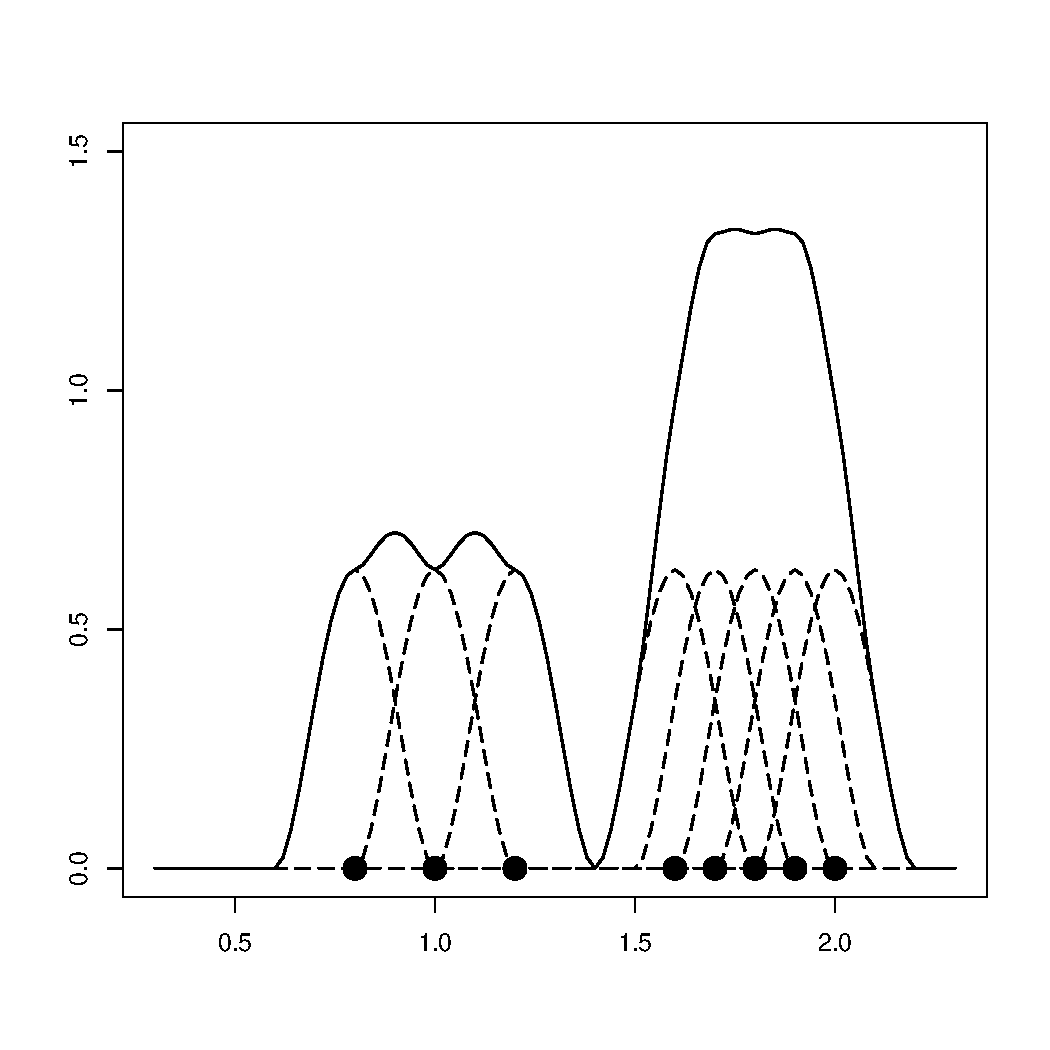
\includegraphics[width=\textwidth]{img/kernel1d-02}
        \subcaption{$h=0.2$}
        \label{fig:theory:kernel1d:02}
    \end{subfigure}
    \begin{subfigure}[t]{0.32\textwidth}
        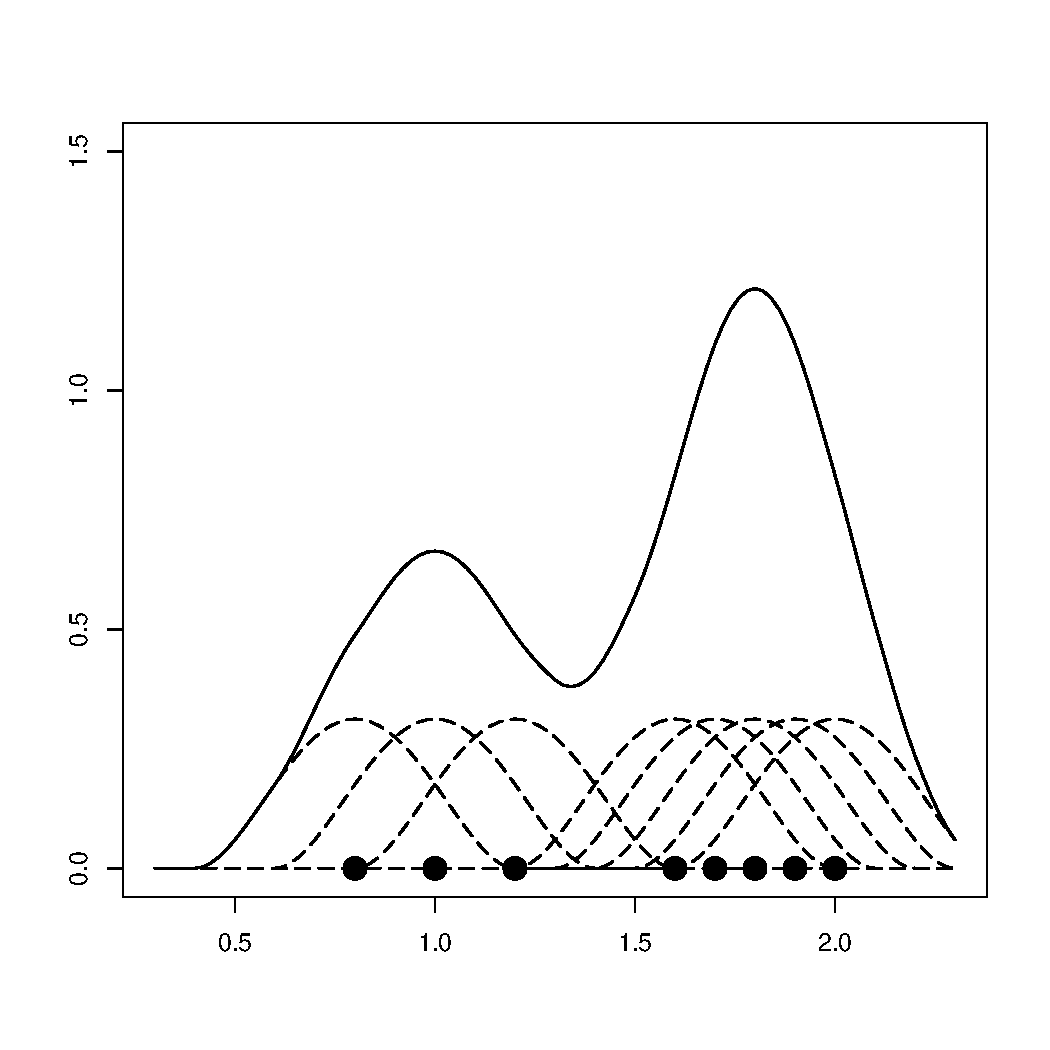
\includegraphics[width=\textwidth]{img/kernel1d-04}
        \subcaption{$h=0.4$}
        \label{fig:theory:kernel1d:04}
    \end{subfigure}
    \begin{subfigure}[t]{0.32\textwidth}
        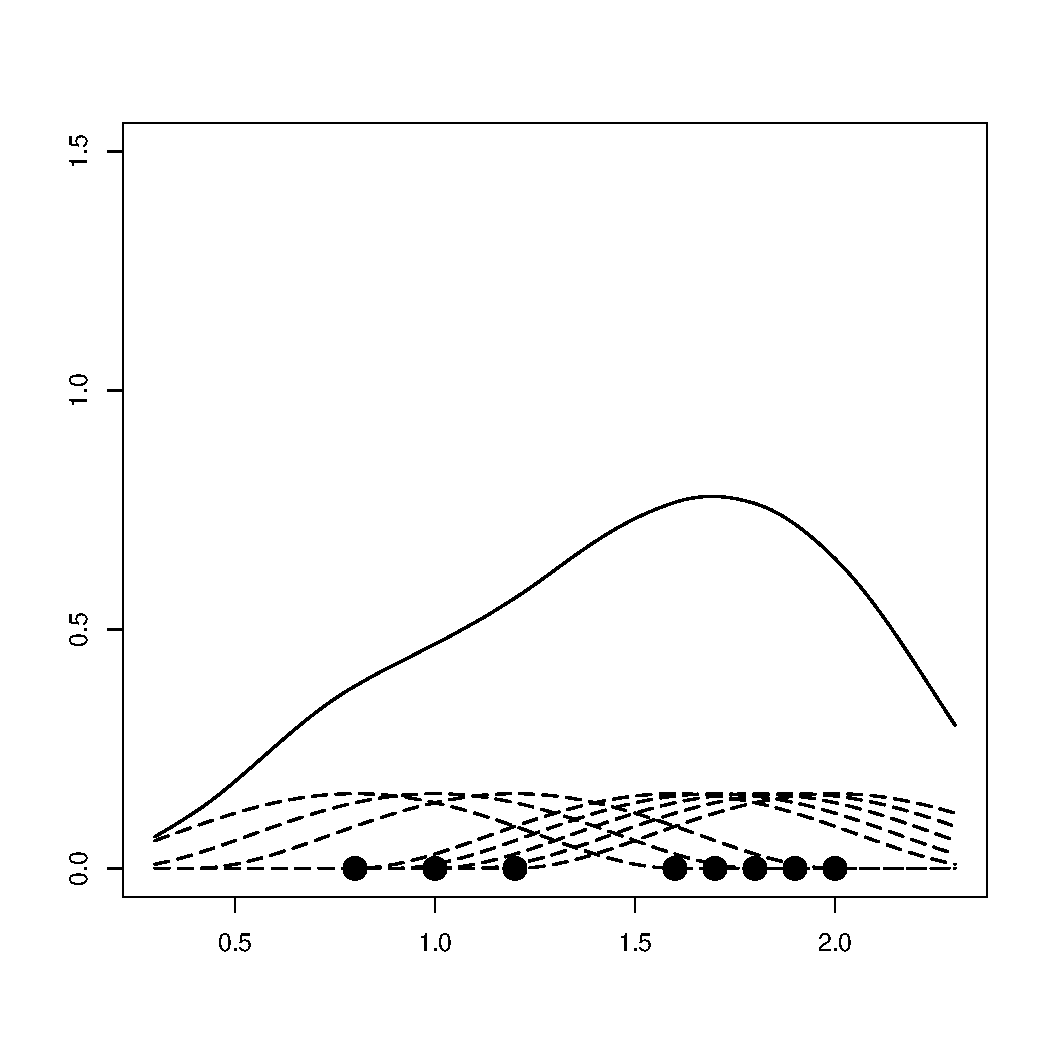
\includegraphics[width=\textwidth]{img/kernel1d-08}
        \subcaption{$h=0.8$}
        \label{fig:theory:kernel1d:08}
    \end{subfigure}
    \caption[One-dimensional \glsentryname{kernel} functions]
        {One-dimensional \glsentryname{kernel} functions using the biweight(quartic) kernel \citep{silverman1986density}.
        The dots on the $x_1$ axis are the observed \glsentryplural{event}.
        The dashed lines are the kernel functions around these \glsentryplural{event}
        and the solid line is the \glsentryname{intensity} estimate $\hat{\lambda_1}$.}
    \label{fig:theory:kernel1d}
\end{figure}

\Cref{fig:theory:kernel1d} shows an example of how \gls{kernel} smoothing works in  one-dimension for three different bandwidths.
The dots along the bottom are the observed \glspl{event}.
The dashed lines show the \gls{kernel} functions around each of these \glspl{event},
while the upper solid line is the \gls{intensity} estimate produced using \Cref{eq:lambda_hat_1}.
\Cref{fig:theory:kernel1d:02} shows the estimate with $h=0.2$.
It has two local modes, each with a bit of fluctuation at the peaks.
In \Cref{fig:theory:kernel1d:04} we still see two modes with $h=0.4$, but with smoother peaks.
\Cref{fig:theory:kernel1d:08} has smoothed the two peaks together into a single,
large peak by using the larger bandwidth of $h=0.8$.

The two-dimensional case is analogous.
Starting with a set of \glspl{event} $\gls{N} \subset \RS$,
and a positive value \gls{h} known as the bandwidth,
we define the the \gls{kernel intensity estimator} as follows:
\begin{defn}
    \label{defn:lambda_hat}
    The \textbf{\gls{kernel intensity estimator}} $\gls{lambda_hat}_h \xvec$
    is a technique for estimating the \gls{intensity} of an \gls{spp}
    from observed \glspl{event} \gls{N}.
    The formula for computing the \gls{kernel intensity estimator} is:
    \begin{equation}
        \label{eq:lambda_hat}
        \gls{lambda_hat}_h \xvec%
            = \sumS{\gls{K}\left( \frac{\xvec-(s_1, s_2)}{h} \right)} \text{.}%
    \end{equation}
\end{defn}
where $\xvec-(s_1, s_2)$ is ordinary vector subtraction,
and $\frac{\xvec-(s_1, s_2)}{h}$ is scalar multiplication by $\frac{1}{h}$.
For the remainder of this section we treat $h$ as a scalar for ease of explanation.
However, with no loss of generality we will use separate bandwidths in each coordinate,
that is $\mathbf{h}=(h_1, h_2)$.

There are many kernels which satisfy \Cref{eq:k_pos,eq:k_1},
including two-dimensional versions of the square kernel, the Gaussian kernel and the Epanechnikov kernel.
In this study we use the two-dimensional biweight kernel,
also known as the quartic kernel,
which can be found in \citet{silverman1986density} with formula
\begin{equation}
    \label{eq:biweightkernel2d}
    K \xvec =%
    \begin{cases}%
        \frac{3}{\pi}\left( 1 - x_1^2 - x_2^2 \right)^2 & \text{if}~x_1^2+x_2^2<1 \\%
        0 & \text{otherwise.}%
    \end{cases}%
\end{equation}
This kernel spreads the weight of each event \xvec~ into a circle of radius one, centered at \xvec.
The effect of the bandwidth $h$ is to change the radius of that circle to $h$.
The advantage of the kernels over the Epanechnikov kernel is that it twice-differentiable.
The advantage over the Gaussian kernel is that it much faster to compute.

%%%%%%%%%%%%%%%%%%%%%%%%%%%%%%%%%%%%%%%%%%%%%%%%%%%%%%%%%%%%%%%%%%%%%%%%%%%%%%
%%
%% Measuring the accuracy of the estimate
%%
%%%%%%%%%%%%%%%%%%%%%%%%%%%%%%%%%%%%%%%%%%%%%%%%%%%%%%%%%%%%%%%%%%%%%%%%%%%%%%%
\section{Measuring the accuracy of the estimate}
\label{sec:theory:accuracy}

This section is based on \citet{silverman1986density} and \citet{wand1994kernel}.
A common statistical problem is to find the ``best'' estimate \gls{lambda_hat}
for the \gls{intensity} of an unknown \gls{spp}
based on a set of observed \glspl{event}.
In order to do this using \gls{kernel intensity estimation},
we must select the ``best'' bandwidth.
From \Cref{fig:theory:kernel1d} we can see that different values of bandwidth \gls{h} result in different estimates for the \gls{intensity}.
Our goal is to find a decision procedure that gives us the ``best'' result.
While there is a great deal of research in \gls{kde},
there is much less work available for \gls{kernel intensity estimation}.
We make use of one such result:
the optimal bandwidth used for computing the \gls{kernel intensity estimator} is the same as that for computing the related \gls{kde} function,
and can be determined by the same techniques \Citep{diggle1988equivalence}.
However, the \gls{kde} is used to estimate a probability density function,
while the \gls{kernel intensity estimator} is used to compute an intensity function.
Computationally, the difference is that a density must integrate to one,
and in order to do that,
we divide by $n$,
the number of observed events.


The first thing we must do is define what we mean by the ``best'' result.
We do this by choosing a measure of accuracy for the estimate,
and selecting the bandwidth which gives the optimal value for this measure.
One common accuracy measure used for function estimation is the \gls{mise},
because it has several useful mathematical properties.
It allows for additional analysis by being broken down into the mean integrated squared bias and mean integrated variance.
It can also be estimated by \acrlong{cv}.

Given a realized estimate \gls{lambda_hat} for any function \gls{lambda},
we can compute the squared error at any given point $\xvec \in \RS$ as
$\left( \lmbdhat - \lmbd \right)^2$,
and its expected value at $\xvec$ is called the \gls{mse}.
However,
we would like to compute the accuracy of the whole function.
We do this by integrating the squared error of the estimate over the study area to obtain the \gls{ise}.
\begin{equation}
\label{eq:ise}
    \mbox{\gls{ise}}(\gls{lambda_hat}) = \iintW{
            \left( \lmbdhat - \lmbd \right)^2
    }
\end{equation}
The \gls{mise} is the expected value of the \gls{ise} over the sample space of realizations of \gls{Lambda}.
\begin{align}
    \mbox{\gls{mise}}(\gls{lambda_hat}) 
        & = \E [\mbox{\gls{ise}}(\gls{lambda_hat})] \nonumber \\
        & = \E \iintW{ \left( \lmbdhat - \lmbd \right)^2 } \label{eq:mise}
\end{align}
The integrand of \Cref{eq:mise} is non-negative.
Therefore, by Fubini's Theorem, we can change the order of integration and expectation.
\begin{align}
    \mbox{\gls{mise}}(\gls{lambda_hat}) 
        & = \iintW{ \E \left( \lmbdhat - \lmbd \right)^2 } \nonumber \\
        & = \iintW{ \mbox{\gls{mse}}(\gls{lambda_hat}, \xvec) } \nonumber
\end{align}

We decompose \gls{mse} into the squared bias and squared variance% (\Cref{eq:mse:biasvariance}),
giving us
\begin{align}
    \mbox{\gls{mise}}(\gls{lambda_hat}) 
        & = \iintW{ \Big( \E\lmbdhat - \lmbd \Big)^2 } \nonumber \\
        & \qquad + \iintW{ \E \Big( \lmbdhat - \E\lmbdhat \Big)^2 } \label{eq:mise:intbiasvariance}
\end{align}
We call the first part of \Cref{eq:mise:intbiasvariance} the \gls{isb} and the second part the \gls{iv}.

%%%%%%%%%%%%%%%%%%%%%%%%%%%%%%%%%%%%%%%%%%%%%%%%%%%%%%%%%%%%%%%%%%%%%%%%%%%%%%
%%
%% Asymptotic behavior of the bandwidth
%%
%%%%%%%%%%%%%%%%%%%%%%%%%%%%%%%%%%%%%%%%%%%%%%%%%%%%%%%%%%%%%%%%%%%%%%%%%%%%%%
\section{Asymptotic behavior}
\label{sec:theory:asymptotic_bandwidth}

For the \gls{kernel intensity estimator},
the \gls{mise} cannot be computed directly.
Instead,
we need to approximate it.
In order to do this,
we compute approximate values of the bias,
the variance,
and finally we can compute the \gls{amise} which is the sum of the approximate variance and the square of the approximate bias.
This allows us to analyze the behavior of the \gls{mise} asymptotically,
with dependence only on the true function $\gls{lambda}\dotdot$ and the kernel $K\dotdot$.

Following \citep{silverman1986density,wand1994kernel},
and based on the equivalence of bandwidths for the \gls{kde} and the\gls{kernel intensity estimator} \citep{diggle1988equivalence},
we begin by using Taylor's Theorem to approximate the \gls{kde}.
Let \gls{f} be a probability density function,
and define the \gls{kde} of \gls{f}:
\begin{equation*}
    \gls{f_hat} \xvec%
            = \sumSn{\gls{K}\left( \frac{\xvec-(s_1, s_2)}{h} \right)} \text{.}%
\end{equation*}
We make the following assumptions about $K\dotdot$
and $f\dotdot$ \citep{silverman1986density,wand1994kernel}:
\begin{assumptions}
    \item $K\dotdot$ is a probability density function with zero mean \label{amise:assumptions:1}
    \item $K\dotdot$ is radially symmetric and has non-zero, finite variance \label{amise:assumptions:2}
    \item $f\dotdot$ has bounded and continuous second derivatives. \label{amise:assumptions:3}
\end{assumptions}

Under these assumptions,
the first term of the Taylor expansion is zero (\cref{amise:assumptions:1,amise:assumptions:3}),
and the second and remainder terms of the Taylor expansion are finite (\cref{amise:assumptions:2}).
The following formulas for the \gls{amise} can be found it \citet[Section 4.3]{silverman1986density}.
\begin{align}
    \mbox{bias}_h \hat{f} \xvec%
        & \approx \frac{1}{2} h^{2} \alpha \nabla^2 f \xvec \nonumber \\%
    \mbox{variance}_h \hat{f} \xvec%
        & \approx n^{-1} h^{-2} \beta f \xvec \nonumber \\%
    \mbox{\gls{amise}}(f; h)%
        & = \frac{1}{4} h^{4} \alpha^2 \iintW{\left( \nabla^2 f \xvec \right)^2 }%
            + n^{-1} h^{-2} \beta \label{eq:amisef}%
\end{align}
where
\begin{align}
    \alpha & = \iintR{x_1^2 K(x_1,x_2)} \text{, since}~K\dotdot~\text{is radially symmetric,} \nonumber \\
    \beta & = \iintR{\Big( K(x_1,x_2) \Big)^2} \text{, and} \nonumber \\
    \nabla^2 f \xvec & = \frac{\diffsq{f}\xvec}{\diff{x_1^2}} + \frac{\diffsq{f}\xvec}{\diff{x_2^2}} \nonumber \text{.}
\end{align}

We note that both $\alpha$ and $\beta$ depend only on \Kdots,
and that $\nabla^2 f$ is the Laplacian operator which is the trace of the Hessian matrix.
We can now take the derivative of \Cref{eq:amisef} by $h$ and set it to zero,
giving us the optimal bandwidth \gls{h_opt}:
\begin{align}
    \gls{h_opt} & = C n^{-\frac{1}{6}}
\end{align}
where $C$ is a constant that depends on $\lambda$ and $K$.
\begin{defn}
    The \gls{mise} \textbf{optimal bandwidth} $\mathbf{\gls{h_opt}}$ is the value of $h$ that minimizes the \gls{mise} of the \gls{kde} for a given probability density function $f$ and kernel function $K$.
\end{defn}
As noted above,
the optimal bandwidth of the \gls{kde} in the \gls{mise} sense is the same for the \gls{kernel intensity estimator}.
For $h < \gls{h_opt}$, the variance will be higher, while $h > \gls{h_opt}$ will result in a higher bias \Citep{rosenblatt1971curve}.

Since we have $\gls{lambda_hat} = n \hat{f}$,
the formula for the \gls{amise} of $\gls{lambda} = \mu f$ is
\begin{align}
    \mbox{bias}_h \gls{lambda_hat} \xvec%
        & \approx \frac{1}{2} h^{2} \alpha \mu \nabla^2 f \xvec \nonumber \\%
    \mbox{variance}_h  \gls{lambda_hat} \xvec%
        & \approx n^{-1} h^{-2} \beta \mu f \xvec \nonumber \\%
    \mbox{\gls{amise}}(\gls{lambda}; h)%
        & = \frac{1}{4} h^{4} \alpha^2 \mu^2 \iintW{\left( \nabla^2 f \xvec \right)^2 }%
            + \mu^2 n^{-1} h^{-2} \beta \label{eq:amiselambda}%
\end{align}

There are other accuracy measures that can be used to evaluate the estimate of the \gls{kernel intensity estimator}.
We discuss some of these in \Cref{sec:method:accuracy}.
Although we use these measures to characterize the behavior of the \gls{kernel intensity estimator} and the \gls{dkd},
our bandwidth is chosen by techniques that try to achieve \gls{h_opt} and minimize \gls{mise}.
However, as noted above,
our approximation \gls{amise} depends on the true risk function \gls{lambda}.


%%%%%%%%%%%%%%%%%%%%%%%%%%%%%%%%%%%%%%%%%%%%%%%%%%%%%%%%%%%%%%%%%%%%%%%%%%%%%%
%%
%% Bandwidth selection from data
%%
%%%%%%%%%%%%%%%%%%%%%%%%%%%%%%%%%%%%%%%%%%%%%%%%%%%%%%%%%%%%%%%%%%%%%%%%%%%%%%
\section{Bandwidth selection from data}
\label{sec:theory:bandwidthselection}

In practice,
researchers typically do not know the true density or intensity functions.
Therefore they cannot compute \gls{h_opt} directly,
and so they use techniques that give them approximations for this value.
In this study,
we do know the true intensity functions,
since we use them to generate data for the simulations.
Therefore we can compute the ``best'' bandwidth by comparing to the actual truth.
We therefore define
\begin{defn}
    the \textbf{\gls{oracle bandwidth}} for a given \gls{intensity} is the bandwidth that minimizes the empirical \gls{mise},
    computed from the data samples generated from the true \gls{intensity} function.
\end{defn}
Other schemes for selecting the bandwidth that are based on a specific data sample will not be as good as the \gls{oracle}.
The two techniques we use are optimized to find a bandwidth that minimizes \gls{mise}.
The selected bandwidth may or may not be close to \gls{h_opt},
depending on the particular sample.
The first technique we will use is known as \textbf{\Gls{silverman}'s Rule of Thumb}.
We use the version for selecting bandwidth in $\RS$,
which has forumula
\begin{equation}
    \label{eq:silverman}
    h_S = 2.04 * \sigma * n^{-1/6}%
\end{equation}
where $n$ is the observed number of incidents,
$\sigma$ the arithmetic mean of $\sigma_{x_1}$ and $\sigma_{x_2}$,
he standard deviations of the $x_1$ and $x_2$ coordinates of the sample points respectively:
\begin{equation*}
    \sigma = \frac{\sigma_{x_1} + \sigma_{x_1}}{2} \text{.}
\end{equation*}
\citet{silverman1986density} shows that for a large class of intensity functions,
including ones based on Gaussian functions,
this bandwidth provides a good approximation to the optimal bandwidth \gls{h_opt}. 

Our second technique is to use leave-one-out \textbf{\gls{cv}} over a set of bandwidths.
We select the bandwidth which minimizes the \gls{cv} error,
which approximates the \gls{mise} (\Cref{eq:mise}).
For the \gls{kde},
he formula for the \gls{cv} error of bandwidth $h$ for \gls{lambda_hat} is
\begin{equation}
    \label{eq:cverror}
    \mbox{\Gls{cv}}%
        = \iintW{\gls{lambda_hat}_h \xvec^2}
        - 2 n^{-1} \sum\limits_{i=1}^n \gls{lambda_hat}_{-i,h}\xvec%
\end{equation}
where $\gls{lambda_hat}_{-i,h}\xvec$ is the \gls{kernel intensity estimator} computed using the bandwidth $h$ and leaving out the $i^\text{th}$ point.
The technique for \gls{kernel intensity estimation} is identical to the \gls{kde},
in the sense that the bandwidths which minimize the \gls{mise} of the \gls{kernel intensity estimator} are the same \citep{brooks1991asymptotic}. 
\Citet{brooks1991asymptotic} show that the \gls{cv} error computed with the selected bandwidth approximates the optimal \gls{ise} very well,
in the sense that
\begin{equation*}
    \frac   {\mbox{\gls{ise}}(\gls{lambda_hat}; h_{\gls{cv}})}%
            {\mbox{\gls{ise}}(\gls{lambda_hat}; \gls{h_opt})}%
            \to 1 ~\text{almost surely.}%
\end{equation*}

%%%%%%%%%%%%%%%%%%%%%%%%%%%%%%%%%%%%%%%%%%%%%%%%%%%%%%%%%%%%%%%%%%%%%%%%%%%%%%
%%
%% Inconsistency of the kernel intensity estimator
%%
%%%%%%%%%%%%%%%%%%%%%%%%%%%%%%%%%%%%%%%%%%%%%%%%%%%%%%%%%%%%%%%%%%%%%%%%%%%%%%
\section{Inconsistency of the kernel intensity estimator}
\label{sec:theory:inconsistency}

The \gls{kde} $\hat{f}$ can be shown to be a consistent estimator of a density function $f$.
\citet{bertrand1978convergence} show that the \gls{kde} converges uniformly to the true function with probability 1 as $n \to \infty$,
while \citet{devroye1985nonparametric} show that the \gls{kde} converges in $L_1$ to the true function with probability 1.
In contrast to density a density function,
where the estimate is normalized by the number of observations,
for a spatial intensity
both the magnitude of the scaling factor \gls{mu} of the true intensity
and the number of observed events $n$ are proportional
to both the time frame of the study or the size of the study area.
Therefore,
in order to discuss the asymptotic behavior of an intensity function,
it makes sense to look at $\gls{mu} \to \infty$.
We describe the behaviour of the \gls{dkd} as \gls{mu} increases in \Cref{sec:results:unifNpop_1h}.
Along these lines,
\citet{guan2008consistent} note that the \gls{kernel intensity estimator}
``is not a consistent estimator of the true intensity''.

We therefore \textit{normalize} our measures of accuracy in two ways.
The first way is to simply divide our approximated \gls{mise} by $\gls{mu}^2$
as suggested by \citet{diggle1988equivalence},
since we know the true function and therefore \gls{mu}.
The second way is to divide, at every point,
the estimation error $\gls{lambda_hat}\xvec - \gls{lambda}\xvec$ by the true value $\gls{lambda}\xvec$.
Our results contain these and similar relative errors for all of the accuracy measures
as described in \Cref{sec:method:accuracy}.

%%%%%%%%%%%%%%%%%%%%%%%%%%%%%%%%%%%%%%%%%%%%%%%%%%%%%%%%%%%%%%%%%%%%%%%%%%%%%%
%%
%% Data generation process
%%
%%%%%%%%%%%%%%%%%%%%%%%%%%%%%%%%%%%%%%%%%%%%%%%%%%%%%%%%%%%%%%%%%%%%%%%%%%%%%%
\section{Data generation process}
\label{sec:theory:data}

We generate data for each experiment using rejection sampling,
based on the technique suggested in \Citet[Section 4.4]{diggle1983spatial},
based on \citet{lewis1979simulation}.
However,
because we are dealing with a \textit{rate} that affects members of a \textit{population},
our algorithm is slightly different.
We proceed in two parts.
First, we generate a population \gls{P} of the chosen size $N_p$ as follows:
\begin{itemize}
    \item If the population is uniform,
            we choose $N_p$ points uniformly in \gls{W}.
        so that we generate the desired population count $N_P$.
    \item If the population is peaked,
            we choose $N_p$ points from a bivariate normal distribution,
            centered at $(c_1, c_2)$,
            with covariance matrix
            $\begin{pmatrix}
                \sigma_1 & 0 \\
                0 & \sigma_2
            \end{pmatrix}$.
\end{itemize}

Once we have a population,
we can repeatedly simulate sample sets of incidents using the following procedure:
\begin{enumerate}
    \item We create the incident intensity function \gls{lambda_I}
        by scaling a function of the desired shape.
        First we divide by $N_P$,
        because we will apply it on all $N_P$ \glspl{event}.
        Then we multiply it by $N_I/\E f$
        so that the expected number of generated \glspl{incident} will be $N_I$.
    \item For each ``person'' $p\!=\!(p_1, p_2) \in \gls{P}$,
        we calculate the \textit{risk} of coming down with the disease $\gls{lambda_I}(p_1, p_2)$
    \item Keep $(p_1, p_2)$ in \gls{I} with probability $\gls{lambda_I}(p_1, p_2)$.
\end{enumerate}

In this way,
when the population is uniformly distributed,
the expected value of the number of \glspl{incident} will be $N_I$,
and they will be distributed according to \gls{lambda_I}.
In cases where the population has a peak,
the risk function \gls{lambda}\dotdot is still the same,
but the number and distribution of events is not according to $N_I$ and \gls{lambda_I}.

Due to the large size of the population,
we use the same \textbf{fixed} population \gls{P} for an entire experiment
in order to perform the experiments in a reasonable amount of time.
Therefore,
we do not study the randomness in the population distribution in this study.

\chapter{Literature review}
\label{ch:literature}
% !TEX root = thesis.tex

%%
%%
%% Literature chapter
%%
%%

Our research is concerned with two-dimensional non-parametric intensity estimation,
that is estimating functions in the plane while making only minimal assumptions about the underlying distribution of the data. 
In particular, we are interested in estimating an incidence rate,
which is the ratio of incidence count and of population which were each individually computed using kernel methods.
This technique has been applied in several areas of spatial analysis including epidemiology.

\section{Spatial pattern analysis}

The estimation of intensity is part of the wider field of spatial pattern analysis.
For event data such as disease incidence,
spatial point processes including Poisson processes are often used to model the statistical and spatial properties of events.
\Citet{diggle1983spatial} is an early publication which extensively covers the spatial-statistical analysis of point patterns such as these.
While there is some theoretical work available for \gls{kernel intensity estimation},
it is usually based on and compared to \acrfull{kde}.
\Gls{kde} is a popular method of non-parametric estimation of probability density functions from observed data.

\section{Kernel density estimation}
 
The primary reference for probability density estimation is \citet{silverman1986density},
which covers both parametric and non-parametric methods.
In particular,
he covers kernel methods,
including the multi-dimensional \gls{kernel intensity estimation} used in this research.
We note that both of our bandwidth selection methods,
the \Gls{silverman} Rule of Thumb and the least-squares \acrlong{cv} are discussed in this book.
The earliest paper to discuss \gls{kde} for probability density functions was by \citet{rosenblatt1956remarks}.
It contains derivations of the bias, variance,
and \acrfull{mise} for general density estimates in one dimension,
and introduces the class of kernel estimates.
\Citet{wand1993comparison} take an in-depth look at smoothing parameters in two dimensions.
In particular,
they find that using a two-dimensional bandwidth vector is adequate for smoothing in each coordinate direction.
In another book, \citet{wand1994kernel}
give a broad overview of kernel methods,
including several techniques for selecting the bandwidth.
In examining how both the \gls{kde} and \gls{kernel intensity estimation} can use data to learn about underlying structure,
they describe how these similar techniques are used in comparison to parametric methods.
In addition to single and multi-variable kernel methods to estimate functions,
they also describe how kernel regression techniques can be used for supervised learning and prediction.

A different perspective can be found in \citet{devroye1985nonparametric},
which analyses non-parametric density estimation from an $L_1$ perspective,
which is in line with our use of the \gls{miae} measure of accuracy.

\section{Kernel intensity estimation}

The idea to use \gls{kernel intensity estimation} to estimate the intensity functions of one-dimensional point processes can be found in \citet{diggle1985kernel}.
Based on the kernel methods described by \citet{rosenblatt1956remarks},
Diggle's paper includes estimates for the \gls{mise} as well as a performance evaluation using simulated data.
The equivalence of the bandwidth in kernel density and intensity was shown in \citet{diggle1988equivalence}.
\Citet{brooks1991asymptotic} show that the \gls{cv} bandwidth is asymptotically optimal,
building on similar results for the \gls{kde} \citep{hall1983large,burman1985data,stone1984asymptotically}.

Unlike the \gls{kde} however,
the \gls{kernel intensity estimator} is not consistent,
meaning that the \gls{mise} does not converge to zero as the number of incidents increases.
There is some work in this area,
with \citet{guan2008consistent} and \citet{fuentes2016consistent} developing techniques for \gls{kernel intensity estimation} that are consistent under certain conditions.
The research mentioned above is mostly concerned with one-dimensional data.
However, kernel technieques have successfully been used in two dimensions as well \citep{scott1992multivariate}.

\section{Application to epidemiology}

Current research in kernel estimation continues.
For example, we see kernel estimation techniques used in epidemiology.
Like our research,
the tutorial paper \citet{davies2018tutorial} looks at using the ratio of two kernel estimates for estimating epidemiological risk functions.
It is based on the technique developed by \citet{bithell1990application} and \citet{bithell1991estimation}.
He computes two \glspl{kde} in order to compare the relative risk between two samples representing the case and control populations on a common study area.
This relative risk ratio represents a different quantity from the incidence rate of our current research.
Because it is a tutorial, \citet{davies2018tutorial} delves into several bandwidth selection techniques,
edge corrections,
and other methods that extend the basic \gls{kde}.

In many studies,
incidents of disease are aggregated together instead of using spatial analysis.
This is referred to as ``zonal analysis'' and suffers from several issues,
mainly due to information that is lost when aggregating and computing \glspl{asr}.
One of the motivations of spatial analysis is to provide more informative results than can be done with aggregation.
An example of how the results of studies based on such aggregation can be misleading can be found in \citet{portnov2007ecological}.

\section{The double kernel}

The \acrfull{dkd} has been used in epidemiological studies since at least 2004 \citep{rushton2004analyzing}.
\citet{kloog2009using} is another recent study which uses the \gls{dkd}.
In particular,\
it identifies the \gls{maup},
which occurs when changes to the arbitrary administration zones that are used to aggregate incidents can result in different observations and findings.
\citet{zusman2012residential} is another study which discusses the advantages of the \gls{dkd} over \glspl{asr}.
A recent examination of the properties of the \gls{dkd} can be found in \citet{zusman2016application}.

While the \gls{dkd} has been used frequently in epidemiological and non-epidemiological spatial analysis,
its statistical properties have not been adequately studied.
In order to understand these properties,
both a theoretical and an empirical analysis is required.
The scope of this research is to provide a beginning to the empirical analysis by studying the sensitivity of the \gls{dkd} to several factors using monte carlo simulations.



\chapter{Research methodology}
\label{ch:method}
% !TEX root = thesis.tex

%%
%%
%% Results chapter
%%
%%


Relative MISE is the mean integrated relative squared error, where the relative squared error is computed in the following manner:
\[ \mbox{RSE}(x) = \left(\frac{\hat{f}(x)-f(x)}{f(x)}\right)^2 .\]
More generally, the relative error at a point \(x\) is computed as
\[ \mbox{RE}(x) =  \frac{\hat{f}(x)-f(x)}{f(x)} .\]
\autoref{fig:ise:unif_100_unif} shows the empirical distribution of the MISE and RMISE for the uniform intensity on uniform population.
The next row is the mean integrated absolute error (MIAE), which is followed by Relative MIAE which is computed analogously to Relative MISE.
This is followed by the Maximum error, which is the greatest absolute error over the study area.

\chapter{Results}
\label{ch:results}
% !TEX root = thesis.tex

%%
%%
%% Results chapter
%%
%%

This chapter describes the results of several experiments, each run with a variation of the same setup.
In each case, we compare the results of 1,000 simulations using several accuracy measures.
Each section describes a set of experiments, which, together, examine the effect of changes to a single variable on the performance of the \gls{dkd}.

%%%%%%%%%%%%%%%%%%%%%%%%%%%%%%%%%%%%%%%%%%%%%%%%%%%%%%%%%%%%%%%%%%%%%%%%%%%%%%
%%
%% Section: Experimental setup
%%
%%%%%%%%%%%%%%%%%%%%%%%%%%%%%%%%%%%%%%%%%%%%%%%%%%%%%%%%%%%%%%%%%%%%%%%%%%%%%%
\section{Experimental setup}
\label{sec:results:setup}

Each experiment was run on one of \textit{c4.2xlarge} or \textit{c4.4xlarge} instance in Amazon AWS \citep{aws:instancetypes}.
These virtual machines have 8 and 16 virtual CPUs respectively.
This allowed the monte carlo simulations to be sped up by running in 7 or 15 parallel threads using the \texttt{parallel} package in \texttt{R} \citep{r:parallel}.
Randomization in parallel requires the random number stream to be split into separate sub-streams for each thread. 
This was done using the L'Ecuyer-CMRG method \citep{lecuyer2002random}.

Each experiment was run according to a set of parameters that comprised the particular setup.
The parameters (\cref{tab:experimental_parameters}) that define the study area remained fixed throughout the study.
In particular, we set \texttt{x1.min} to -4, \texttt{x1.max} to 4, \texttt{x2.min} to -4, \texttt{x2.max} to 4, and \texttt{buffer} to 0.5.
This gave us a study area with dimensions $8 \times 8$, with incidents concentrated in an area of $7 \times 7$.
For evaluating the \gls{dkd} we used a grid size of 0.5.

A table similar to \cref{tab:params:template}, describing the parameter ranges used in the related experiments appears at the beginning of each section below.
This table summarizes the values from \cref{tab:experimental_parameters} that are used to run the experiments in that section.
The first row in the table contains the \textit{population size} or \textit{sizes} used in the experiment.
The second row contains the \textit{population \gls{spread}}, which controls how quickly the population density drops from the peak.
We use the standard deviation \ensuremath\sigma of an independent, bivariate normal distribution with equal variances for this.
The third row in the the table contains the \textit{population center}, which is the point $\xvec$ of the peak of the population distribution.
For a uniform population distribution, the word ``uniform'' appears.
The next row in the table is the \gls{factor}.
This value is used to increase the expected number of cases for each simulation in the experiment.
It is the same \gls{mu} found in \cref{ch:method}.
The fifth row contains the \textit{incident \gls{spread}}, which controls how quickly the incidence risk drops from the peak.
We use the standard deviation \ensuremath\sigma of an independent, bivariate normal distribution with equal variances for this.
The sixth and last row in the the table contains the \textit{incident center}, which is the point $\xvec$ of the peak of the incident risk function.

%%%%%%%%%%%%%%%%%%%%%%%%%%%%%%%%%%%%%%%%%%%%%%%%%
% Parameter table - template
%%%%%%%%%%%%%%%%%%%%%%%%%%%%%%%%%%%%%%%%%%%%%%%%%
\begin{table}[htbp]
    \centering
    \begin{tabular}{ll}
        \toprule
        Parameter & Value \\
        \midrule
        Population size & 10,000 \\
        Population \glsentryname{spread} & 1.0 \\
        Population center & (0,0) \\
        \Glsentryname{factor} & 100, 200 \\
        Incident \glsentryname{spread} & 1.0 \\
        Incident center & (0,0) \\
        \bottomrule
    \end{tabular}
    \caption{Experimental parameters template and example values}
    \label{tab:params:template}
\end{table}

In \cref{sec:results:unif_100_1.0_1h} we take a deep look at a single experiment.
The rest of this chapter examines the effect of different variables on the \gls{dkd} accuracy, on the selected bandwidths, and on other statistical properties of the \gls{dkd}.
\Cref{sec:results:number_of_incidents} describes the relationship between the accuracy of the \gls{dkd} and the magnitude of the risk function for a fixed population.
In \cref{sec:results:spread} we look at how the spread of the risk function affects accuracy.
We then made ran several sets of experiments while changing one parameter at a time.
\Cref{sec:results:unifNpop_1h} compares the results obtained by varying the size of the population.

%%%%%%%%%%%%%%%%%%%%%%%%%%%%%%%%%%%%%%%%%%%%%%%%%%%%%%%%%%%%%%%%%%%%%%%%%%%%%%
%%
%% Section: Results of single-peak risk on uniform population
%%
%%%%%%%%%%%%%%%%%%%%%%%%%%%%%%%%%%%%%%%%%%%%%%%%%%%%%%%%%%%%%%%%%%%%%%%%%%%%%%
\section[Results of single-peak risk on uniform population]
    {Results of a single experiment with risk function having single peak with with \glsentryname{spread} 1.0 and \glsentryname{factor} of 100 on a fixed, uniform population of 10,000}
\label{sec:results:unif_100_1.0_1h}
\graphicspath{{./results/unif_100_1.0_1h/}}
\makeatletter
\def\input@path{{./results/unif_100_1.0_1h/}}
\makeatother

In this section, we look at how well the \gls{dkd} performs when there is a single, central cause of disease incidents.
The strength of this source to generate incidents degrades with the distance from it.
We simulate this phenomenon with a risk function having a single peak with with \glsentryname{spread} 1.0 and \glsentryname{factor} of 100 on a fixed, uniform population of 10,000.
These parameters are summarized in \cref{tab:params:unif_100_1.0_1h}.
\Cref{fig:cases_scatter:unif_100_1.0_1h} shows a realization, generated from the model.
The distribution of the population in \subref{fig:cases_scatter:unif_100_1.0_1h:popdist},
the population points that were generated in \subref{fig:cases_scatter:unif_100_1.0_1h:poppts},
and the incidents on top of the population in \subref{fig:cases_scatter:unif_100_1.0_1h:incidentspts}.

%%%%%%%%%%%%%%%%%%%%%%%%%%%%%%%%%%%%%%%%%%%%%%%%%
% Parameter table - unif_100_1.0_1h
%%%%%%%%%%%%%%%%%%%%%%%%%%%%%%%%%%%%%%%%%%%%%%%%%
\begin{table}[htbp]
    \centering
    \begin{tabular}{ll}
        \toprule
        Parameter & Value \\
        \midrule
        Population size & 10,000 \\
        Population \glsentryname{spread} & uniform \\
        Population center & uniform \\
        \Glsentryname{factor} & 100 \\
        Incident \glsentryname{spread} & 1.0 \\
        Incident center & (0,0) \\
        \bottomrule
    \end{tabular}
    \caption[Parameters of single-peak risk of 100 on uniform population]
        {Parameters used in a single experiment with a single-peak risk of \glsentryname{factor} 100 with \glsentryname{spread} of 1.0 on uniform population of 10,000.}
    \label{tab:params:unif_100_1.0_1h}
\end{table}


%%%%%%%%%%%%%%%%%%%%%%%%%%%%%%%%%%%%%%%%%%%%%%%%%
% Example cases scatter - unif_100_1.0_1h
%%%%%%%%%%%%%%%%%%%%%%%%%%%%%%%%%%%%%%%%%%%%%%%%%
\begin{figure}[htbp]
    \centering
    \begin{subfigure}[t]{0.32\textwidth}
        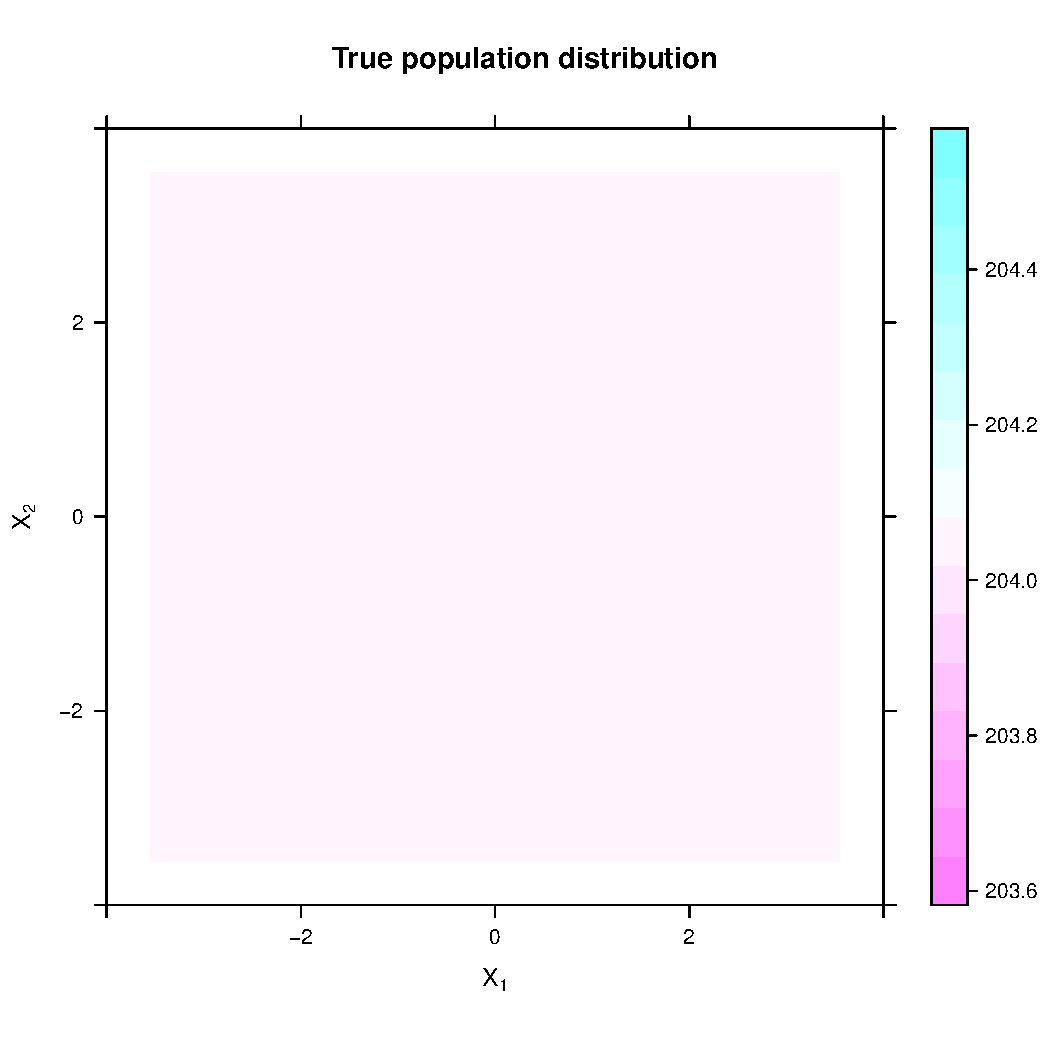
\includegraphics[width=\textwidth]{output/population-heatmap}
        \subcaption{Population distribution}
        \label{fig:cases_scatter:unif_100_1.0_1h:popdist}
    \end{subfigure}
    \begin{subfigure}[t]{0.32\textwidth}
        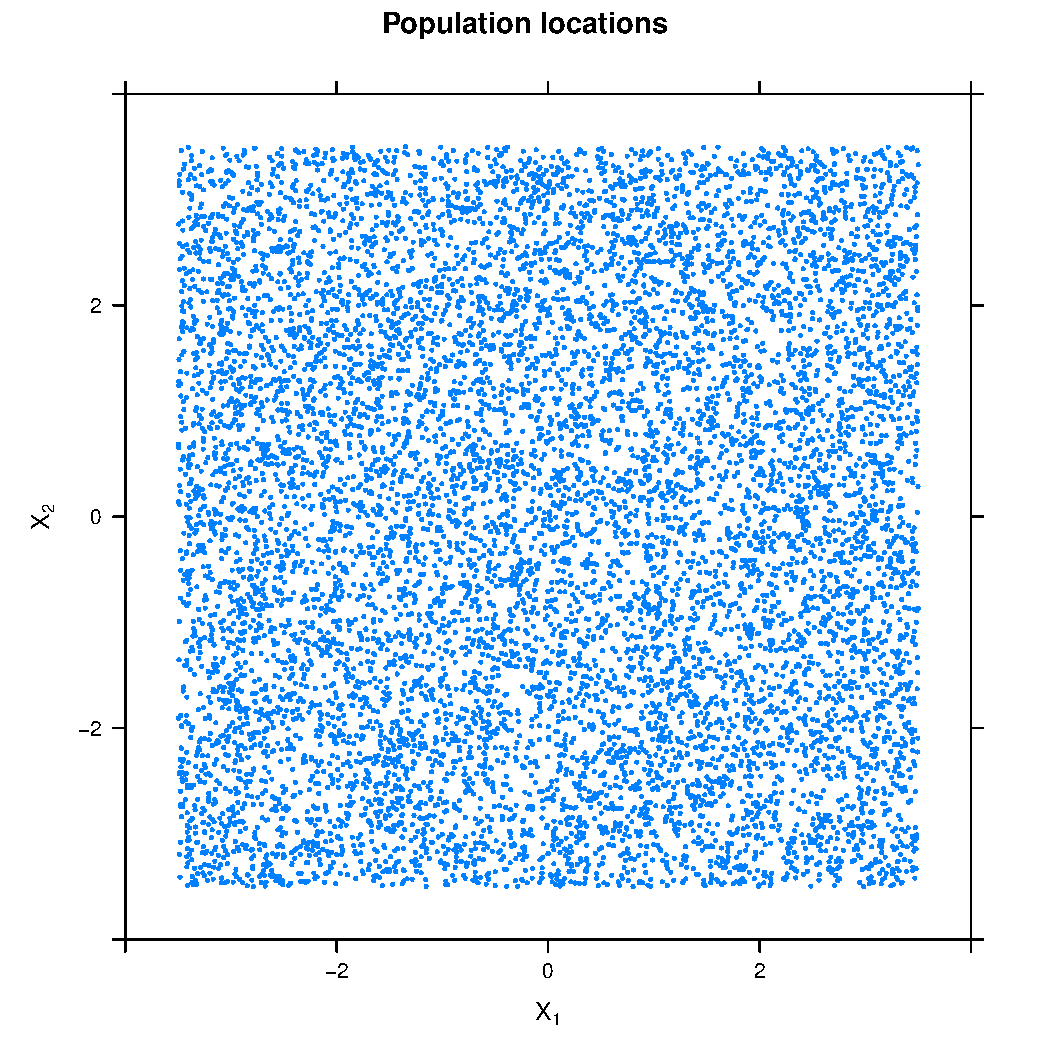
\includegraphics[width=\textwidth]{output/population-points}
        \subcaption{Population realization}
        \label{fig:cases_scatter:unif_100_1.0_1h:poppts}
    \end{subfigure}%
    \begin{subfigure}[t]{0.32\textwidth}
        \includegraphics[width=\textwidth]{output/population_and_incidents_scatter}
        \subcaption{With incidents}
        \label{fig:cases_scatter:unif_100_1.0_1h:incidentspts}
    \end{subfigure}%
    \caption[Example population and incidents: single-peak risk on uniform population]
        {Example population and incidents of one realization of single-peak risk of \glsentryname{factor} 100 with \glsentryname{spread} of 1.0 on a uniform population of 10,000. The red dots are the true peak. The blue diamonds are the peaks of the estimates. The black crosses are the centroid peaks of the estimates.}
    \label{fig:cases_scatter:unif_100_1.0_1h}    
\end{figure}

%%%%%%%%%%%%%%%%%%%%%%%%%%%%%%%%%%%%%%%%%%%%%%%%%
% Example cases heat map - unif_100_1.0_1h
%%%%%%%%%%%%%%%%%%%%%%%%%%%%%%%%%%%%%%%%%%%%%%%%%
\begin{figure}[htbp]
    \centering
    \begin{subfigure}[t]{0.45\textwidth}
        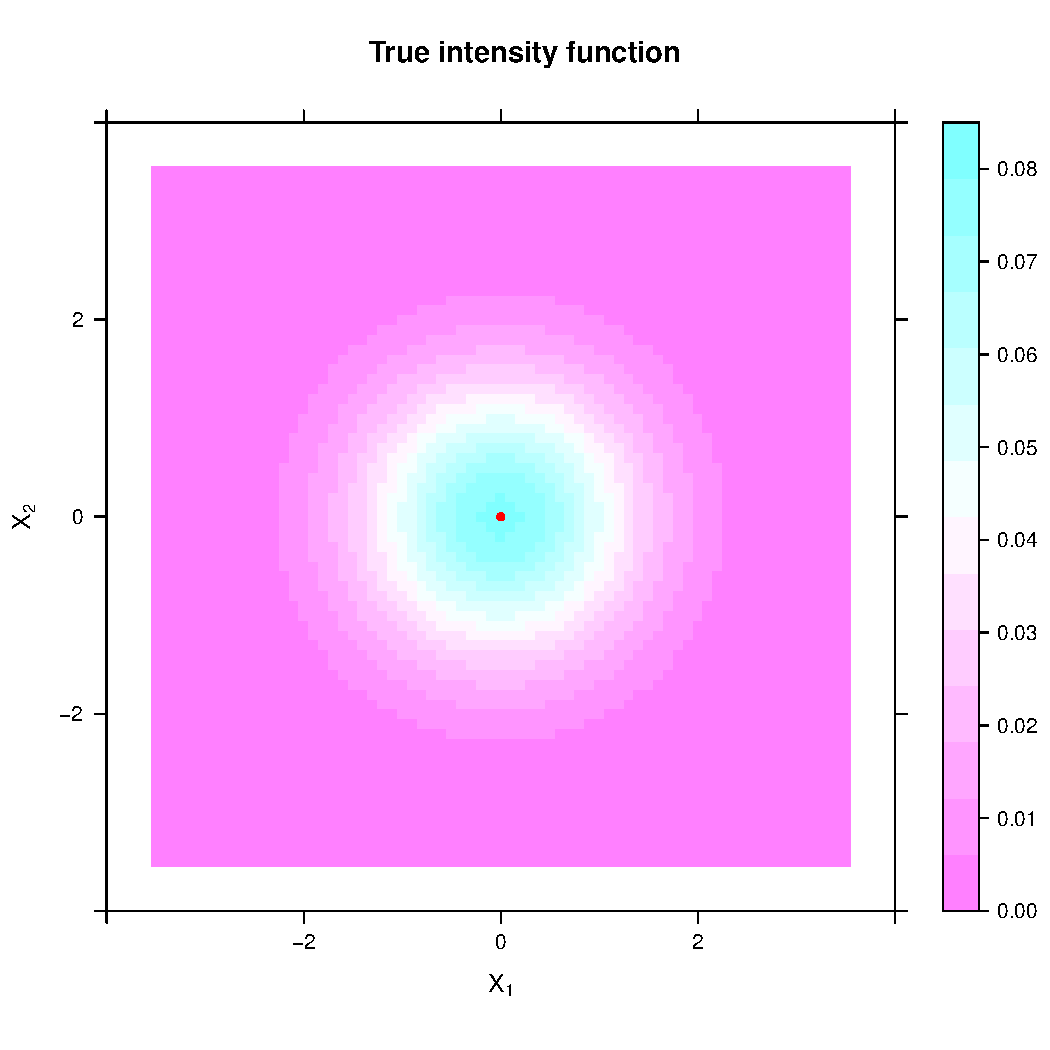
\includegraphics[width=\textwidth]{output/true_intensity_heatmap}
        \subcaption{True incident risk function}
        \label{fig:cases_heatmap:unif_100_1.0_1h:true}
    \end{subfigure}%
    \begin{subfigure}[t]{0.45\textwidth}
        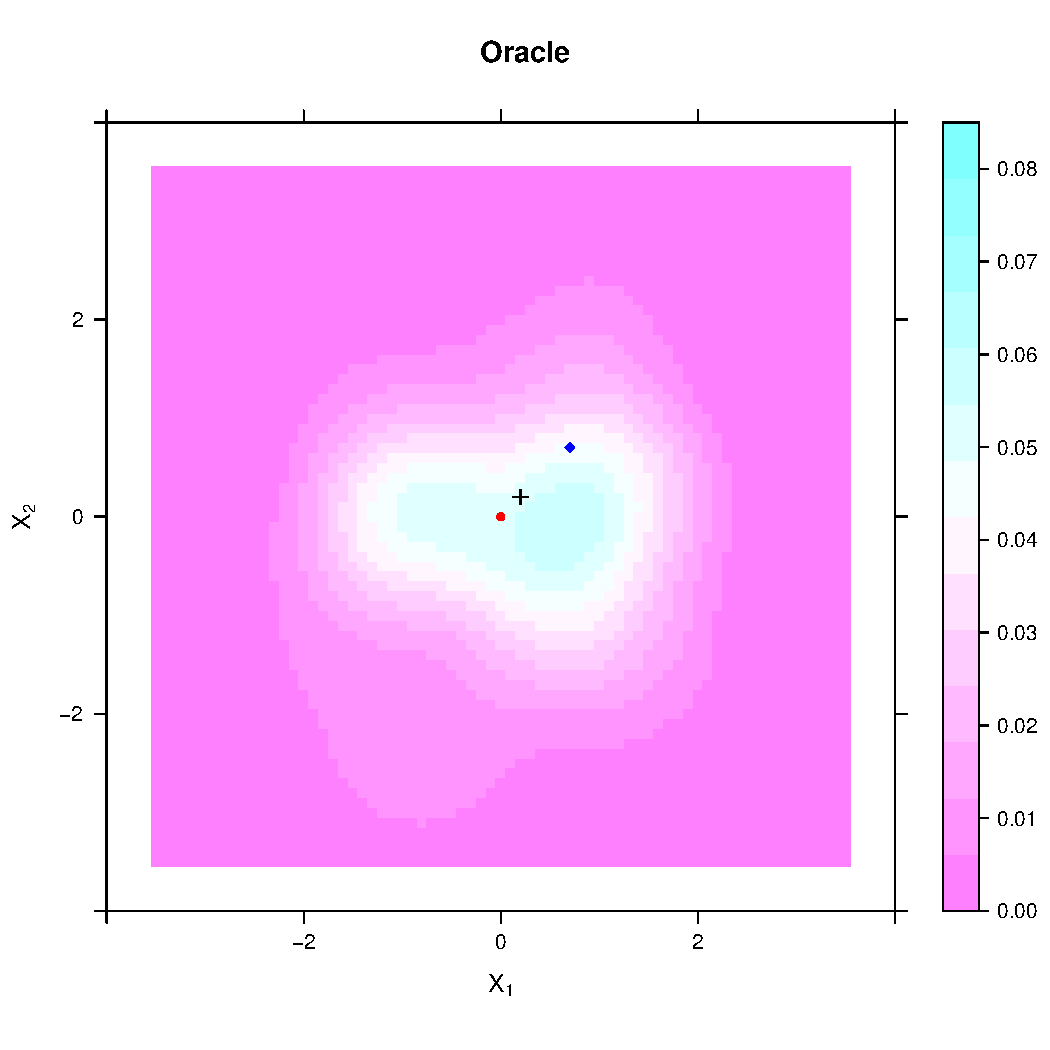
\includegraphics[width=\textwidth]{output/oracle_intensity_heatmap}
        \subcaption{Incident risk estimate using Oracle bandwidth}
        \label{fig:cases_heatmap:unif_100_1.0_1h:oracle}
    \end{subfigure}

    \begin{subfigure}[b]{0.45\textwidth}
        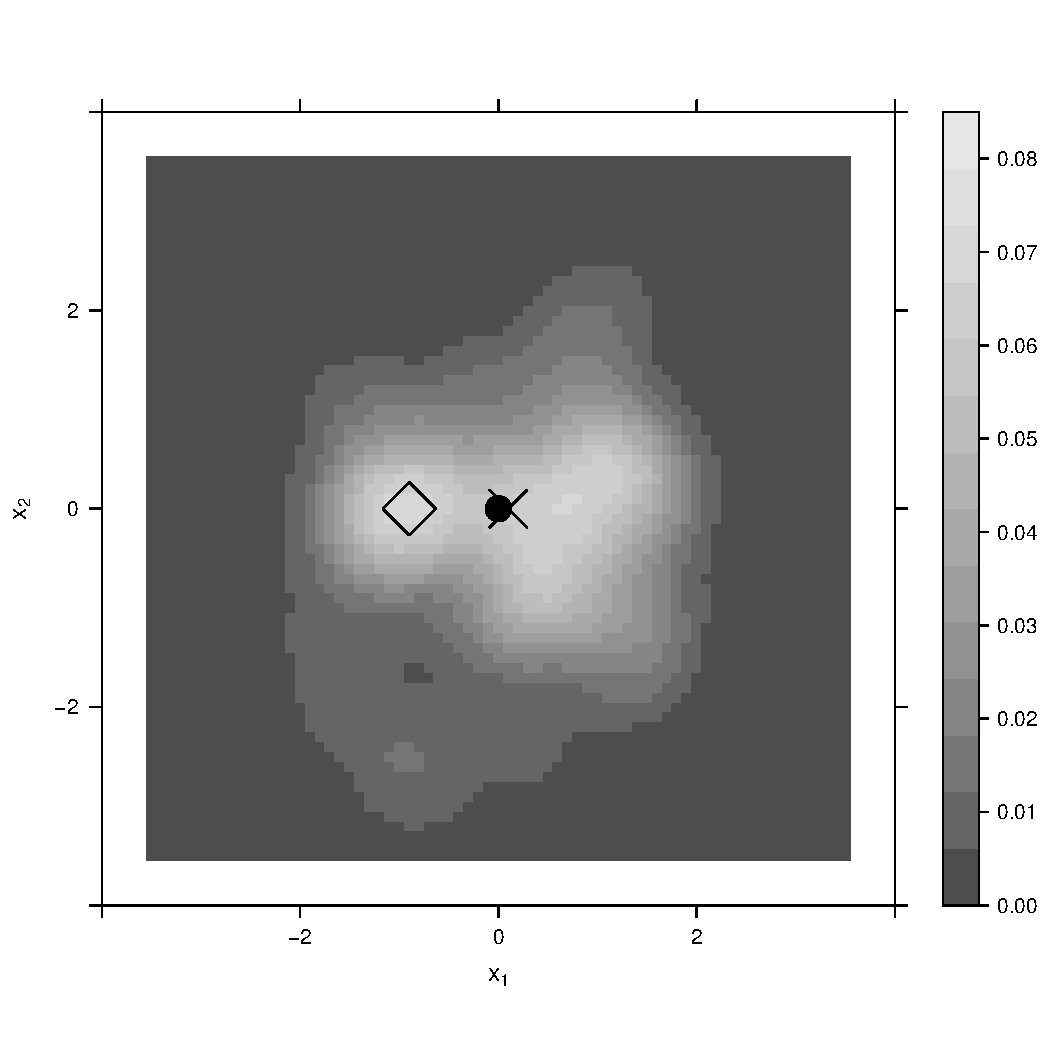
\includegraphics[width=\textwidth]{output/silverman_intensity_heatmap}
        \subcaption{Incident risk estimate using Silverman bandwidth}
        \label{fig:cases_heatmap:unif_100_1.0_1h:silverman}
    \end{subfigure}%
    \begin{subfigure}[b]{0.45\textwidth}
        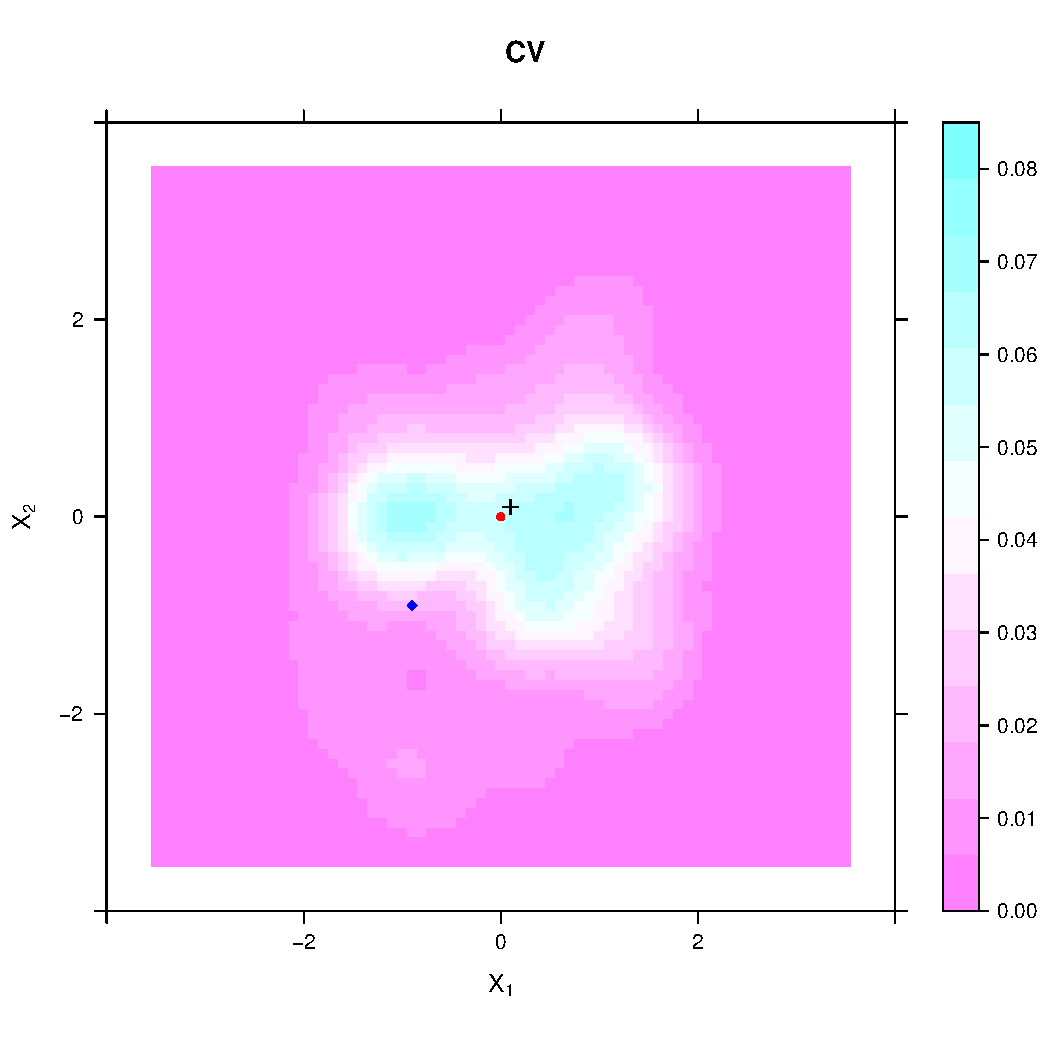
\includegraphics[width=\textwidth]{output/CV_intensity_heatmap}
        \subcaption{Incident risk estimate using Cross-validation bandwidth}
        \label{fig:cases_heatmap:unif_100_1.0_1h:cv}
    \end{subfigure}
    \caption[Example incidents: uniform incident risk on uniform population, 100 cases]
        {Example incidents: uniform incident risk on uniform population, 100 cases}
    \label{fig:cases_heatmap:unif_100_1.0_1h}
\end{figure}

In order to better understand the incident risk and the estimates,
we use a two-dimensional geographic heatmap of the study area \gls{W} to show a single simulation realization in
\cref{fig:cases_heatmap:unif_100_1.0_1h}.
The color of a point $\xvec$ represents the risk or estimated risk of an incident at that point.
\Cref{fig:cases_heatmap:unif_100_1.0_1h:true} shows a heatmap of the true distribution function.
We see the \gls{dkd} estimates obtained using the \gls{oracle} in \subref{fig:cases_heatmap:unif_100_1.0_1h:oracle},
\gls{silverman} in \subref{fig:cases_heatmap:unif_100_1.0_1h:silverman} and \gls{cv} in \subref{fig:cases_heatmap:unif_100_1.0_1h:cv}.
The red dot is the location of the true peak.
The blue diamond is the location of the estimated peak,
and the black cross is the location of the centroid estimated peak.

%%%%%%%%%%%%%%%%%%%%%%%%%%%%%%%%%%%%%%%%%%%%%%%%%
% Mean errors - unif_100_1.0_1h
%%%%%%%%%%%%%%%%%%%%%%%%%%%%%%%%%%%%%%%%%%%%%%%%%
\begin{table}[htbp]
    \centering
    % latex table generated in R 3.4.2 by xtable 1.8-2 package
% Sat Feb 17 16:44:44 2018
\begin{tabular}{lrrr}
  \hline
 & Oracle & Silverman & CV \\ 
  \hline
MISE & 0.000053 & 0.000083 & 0.000080 \\ 
  Relative MISE & 0.002028 & 0.003195 & 0.003047 \\ 
  Normalized MISE & 0.000026 & 0.000042 & 0.000040 \\ 
  MIAE & 0.003914 & 0.004863 & 0.004653 \\ 
  Relative MIAE & 0.024227 & 0.030102 & 0.028802 \\ 
  Max Error & 0.033855 & 0.049415 & 0.045884 \\ 
  Peak bias & -0.016050 & 0.010816 & -0.002953 \\ 
  Relative Peak bias & -0.099339 & 0.066949 & -0.018278 \\ 
  Peak drift & 0.223424 & 0.357624 & 0.284159 \\ 
  Relative Peak drift & 0.031918 & 0.051089 & 0.040594 \\ 
  Centroid bias & -0.017140 & -0.000902 & -0.013918 \\ 
  Relative Centroid bias & -0.106087 & -0.005583 & -0.086149 \\ 
  Centroid drift & 0.149249 & 0.159867 & 0.152694 \\ 
  Relative Centroid drift & 0.021321 & 0.022838 & 0.021813 \\ 
   \hline
\end{tabular}

    \caption{Mean error rates for uniform population, single-peak risk with \glsentryname{spread} 1.0 of \glsentryname{factor} 100}
    \label{tab:errors:unif_100_1.0_1h}
\end{table}

\Cref{tab:errors:unif_100_1.0_1h} contains a summary of all of the measures of accuracy for this experiment.
We can see that for most measures, the \gls{oracle} selected bandwidth provides the best results.
Since the \gls{oracle} bandwidth is designed to be approximate the \gls{mise}-optimal bandwidth \gls{h_opt},
this is not surprising.
However, in real world scenarios, the true function is unknown, and hence it is impossible to compute the \gls{oracle} bandwidth.
Therefore, we are interested in knowing how close the \gls{silverman} and \gls{cv} bandwidth selection methods can get to the \gls{oracle} for the different measures.
One exception is the \gls{peak bias}, which measures the difference between the maximum of the estimated risk and the maximum of the true risk (see \cref{subsec:method:peak_bias}).
In this experiment, the \gls{silverman} and \gls{cv} bandwidths produced lower absolute \gls{peak bias} values than the \gls{oracle}. 
However, the \gls{oracle} and \gls{cv} bandwidths resulted in negative biases,
which is what we expected,
since the process of smoothing generally lowers high values (peaks) and raises low values.
The \gls{silverman} bandwidth, on the other hand, produced a positive value,
which may indicate undersmoothing.
This requires further study.

In \cref{fig:ise:unif_100_1.0_1h}, we look at the distribution of the \gls{ise}.
As described in \cref{subsec:method:mise},
the \gls{iae} gives a summary of the error of the estimate over all of \gls{W},
that penalizes higher error values.
In particular, we see that the relative and normalized \gls{ise} have similarly shaped distributions, although the scale is different.
We also observe that the distributions are skewed to the right,
indicating that for this simple setup,
the accuracy of the \gls{dkd} for a specific sample is more likely to be below the \gls{mise}.
Finally, we note that the estimates calculated with \gls{silverman} and \gls{cv}
selected bandwidths and their corresponding mean values had similar performance in \gls{ise}.

%%%%%%%%%%%%%%%%%%%%%%%%%%%%%%%%%%%%%%%%%%%%%%%%%
% ISE distribution - unif_100_1.0_1h
%%%%%%%%%%%%%%%%%%%%%%%%%%%%%%%%%%%%%%%%%%%%%%%%%
\begin{figure}[htbp]
    \centering
    \begin{subfigure}[b]{0.45\textwidth}
        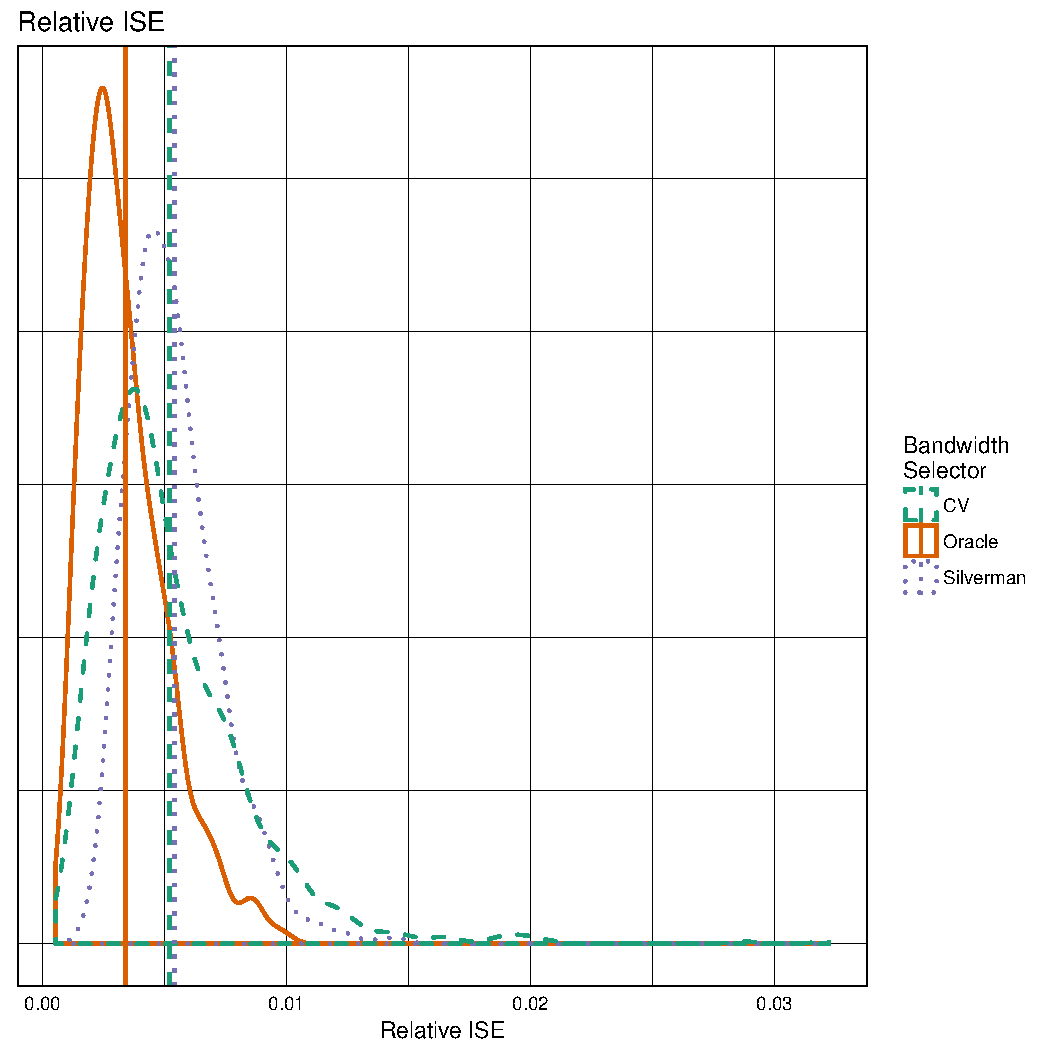
\includegraphics[width=\textwidth]{output/ise-relative-histogram}
        \subcaption{Relative \glsentryname{ise}}
    \end{subfigure}
    \begin{subfigure}[b]{0.45\textwidth}
        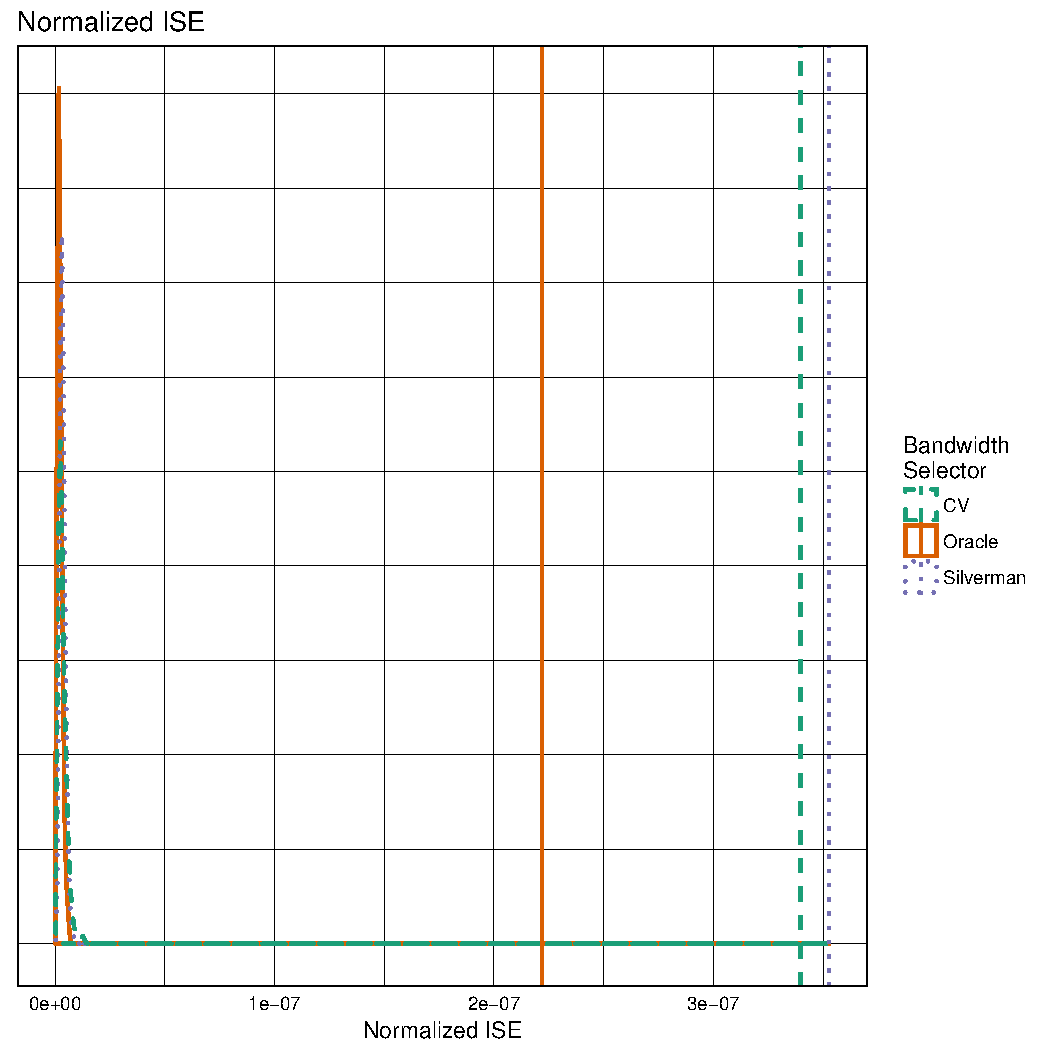
\includegraphics[width=\textwidth]{output/ise-normalized-histogram}
        \subcaption{Normalized \glsentryname{ise}}
    \end{subfigure}
    \caption[\glsentryname{ise}: Single-peak of 100 on uniform population]{\glsentryname{ise} density for a single-peak intensity with \glsentryname{spread} of 1.0 and \glsentryname{factor} of 100 on a uniform population. Vertical lines indicate the estimated \glsentryname{mise} of the simulations. \glsentryname{nmise} values are multiplied by $10^9$.}
    \label{fig:ise:unif_100_1.0_1h}
\end{figure}

%%%%%%%%%%%%%%%%%%%%%%%%%%%%%%%%%%%%%%%%%%%%%%%%%
% IAE distribution - unif_100_1.0_1h
%%%%%%%%%%%%%%%%%%%%%%%%%%%%%%%%%%%%%%%%%%%%%%%%%
\begin{figure}[htbp]
    \centering
    \begin{subfigure}[b]{0.45\textwidth}
        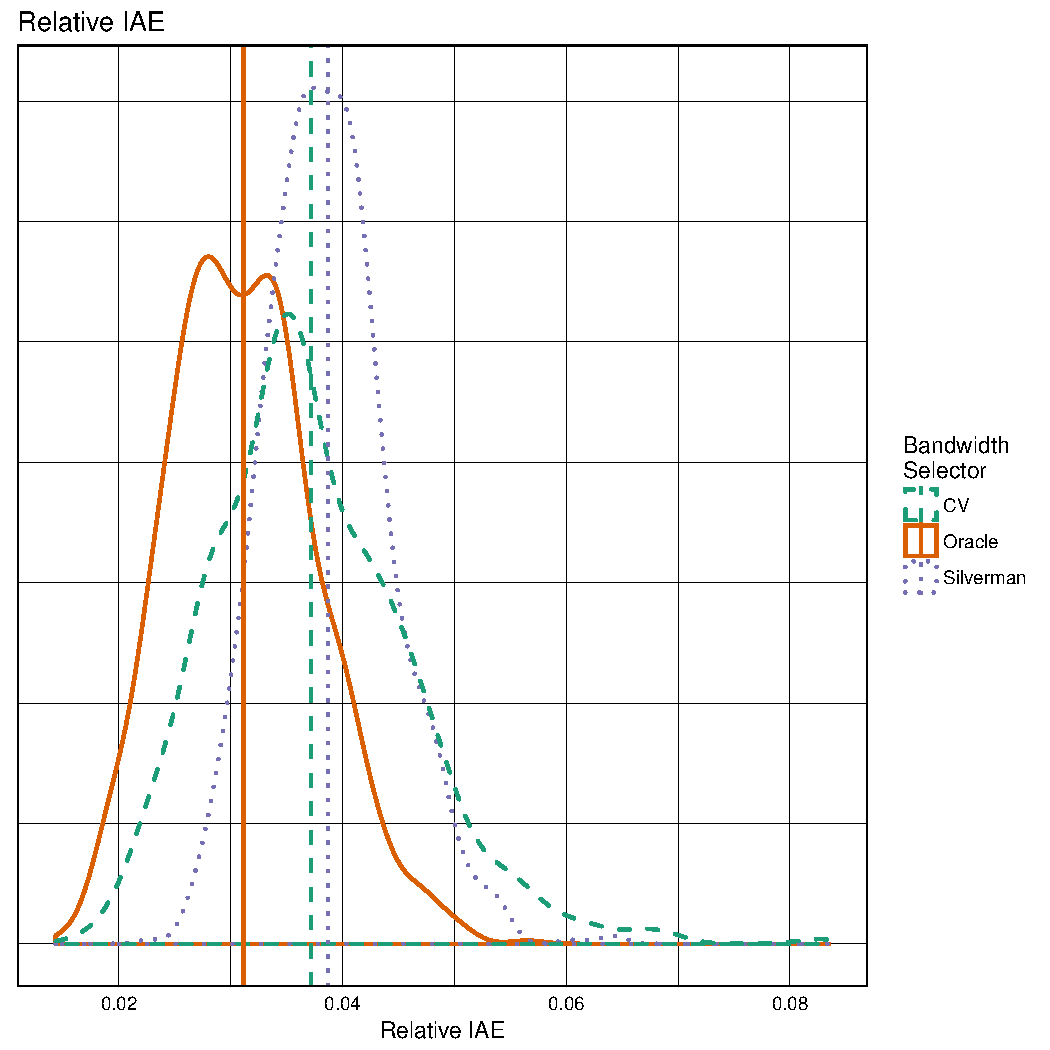
\includegraphics[width=\textwidth]{output/iae-relative-histogram}
        \subcaption{Relative \glsentryname{iae}}
    \end{subfigure}
    \begin{subfigure}[b]{0.45\textwidth}
        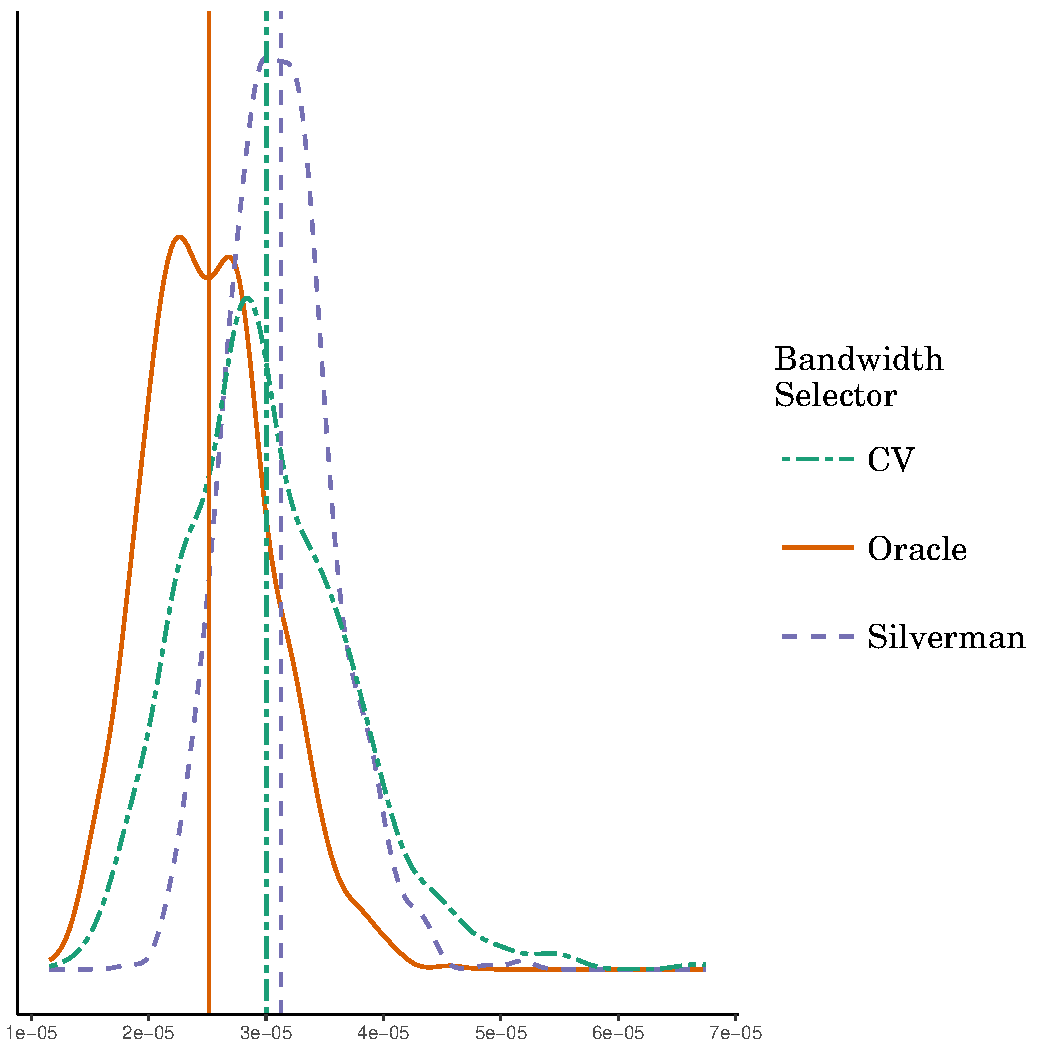
\includegraphics[width=\textwidth]{output/iae-normalized-histogram}
        \subcaption{Normalized \glsentryname{iae}}
    \end{subfigure}
    \caption[\glsentryname{iae}: Single-peak of 100 on uniform population]{\glsentryname{iae} density for a single-peak intensity with \glsentryname{spread} of 1.0 and \glsentryname{factor} of 100 on a uniform population. Vertical lines indicate the estimated \glsentryname{miae} of the simulations.}
    \label{fig:iae:unif_100_1.0_1h}
\end{figure}

%%%%%%%%%%%%%%%%%%%%%%%%%%%%%%%%%%%%%%%%%%%%%%%%%
% Max error distribution - unif_100_1.0_1h
%%%%%%%%%%%%%%%%%%%%%%%%%%%%%%%%%%%%%%%%%%%%%%%%%
\begin{figure}[htbp]
    \centering
    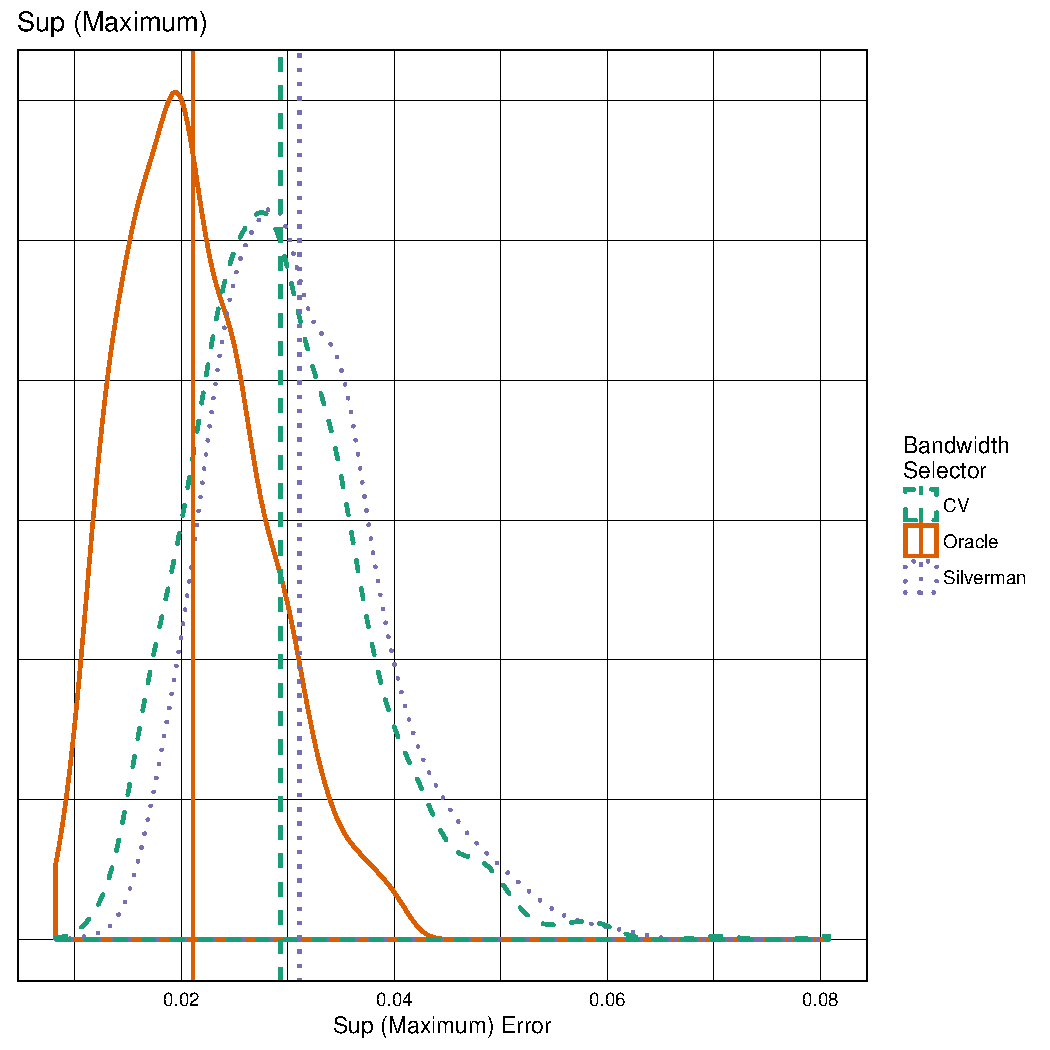
\includegraphics[width=0.45\textwidth]{output/maxerr-histogram}
    \caption[\glsentryname{supremum error}: Single-peak of 100 on uniform population]{\glsentryname{supremum error} density for a single-peak intensity with \glsentryname{spread} of 1.0 and \glsentryname{factor} of 100 on a uniform population. Vertical lines indicate the estimated mean \glsentryname{supremum error} of the simulations.}
    \label{fig:maxerr:unif_100_1.0_1h}
\end{figure}

\Cref{fig:ise:unif_100_1.0_1h} shows the relative and normalized distributions of the \gls{iae}.
As described in \cref{subsec:method:miae},
the \gls{iae} gives a summary of the error of the estimate over all of \gls{W},
giving equal weight to all error values.
Once again, the normalized and relative error measures have similar distributions.
The \gls{oracle} bandwidth selection technique is still notably more accurate when comparing with \gls{iae} than with \gls{ise}.
However, for \gls{iae} we see that \gls{cv} bandwidth selection results in a wider distribution than with \gls{silverman}.

In \cref{fig:maxerr:unif_100_1.0_1h}, we look at the distribution of the \gls{supremum error}.
As described in \cref{subsec:method:sup_error},
the \gls{supremum error} is the worst-case error of the estimate on \gls{W}.
We observe that the distributions are once again skewed to the right,
indicating that for this simple setup,
the worst-case accuracy of the \gls{dkd} for a specific sample is more likely to be below the average \gls{supremum error}.
Finally, we note that the estimates calculated with \gls{silverman} and \gls{cv}
selected bandwidths and their corresponding mean values had similar performance in \gls{supremum error}.


%%%%%%%%%%%%%%%%%%%%%%%%%%%%%%%%%%%%%%%%%%%%%%%%%
% Peaks - unif_100_1.0_1h
%%%%%%%%%%%%%%%%%%%%%%%%%%%%%%%%%%%%%%%%%%%%%%%%%
\begin{figure}[htbp]
    \centering
    \begin{subfigure}[b]{0.45\textwidth}
        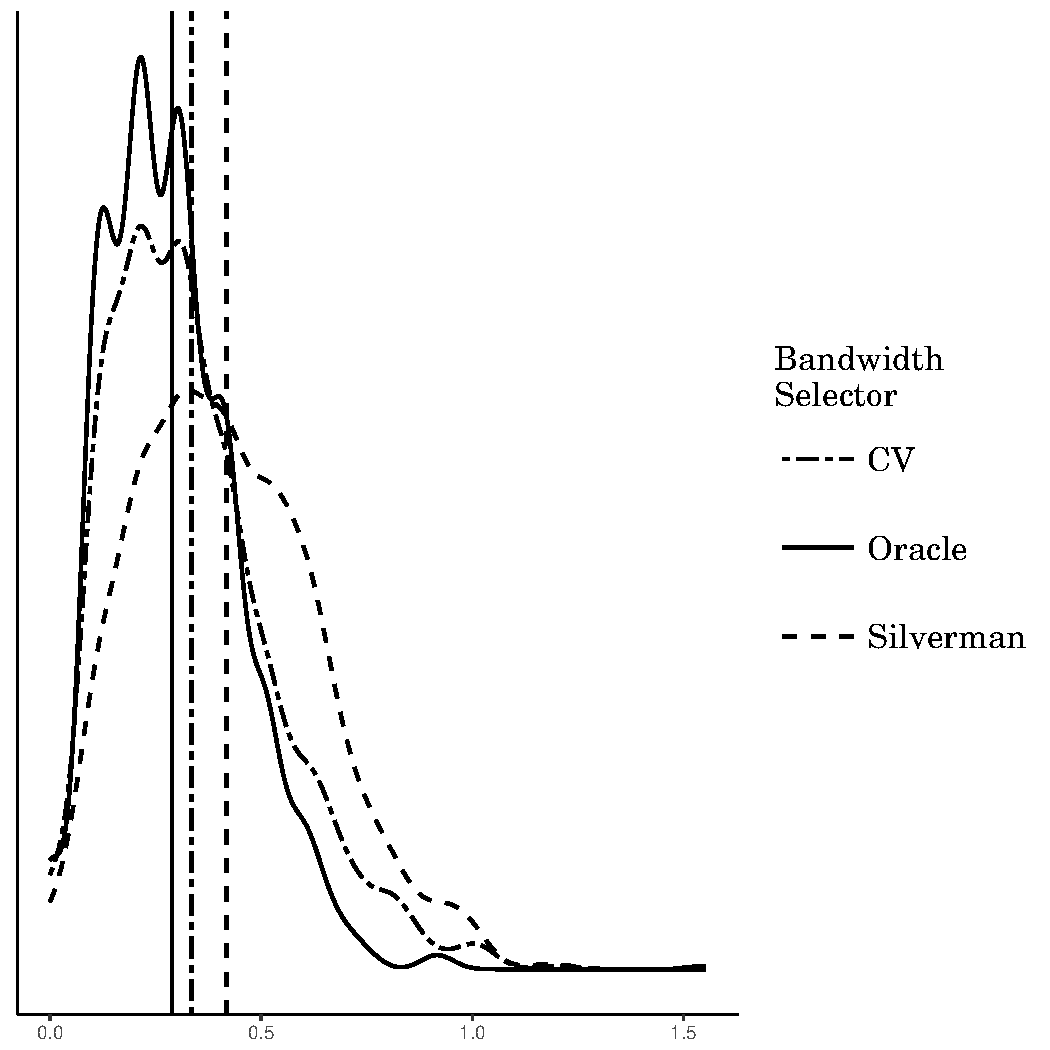
\includegraphics[width=\textwidth]{output/peak-dist-histogram}
        \subcaption{Peak distance from truth}
        \label{fig:peaks:unif_100_1.0_1h:dist}
    \end{subfigure}
    \begin{subfigure}[b]{0.45\textwidth}
        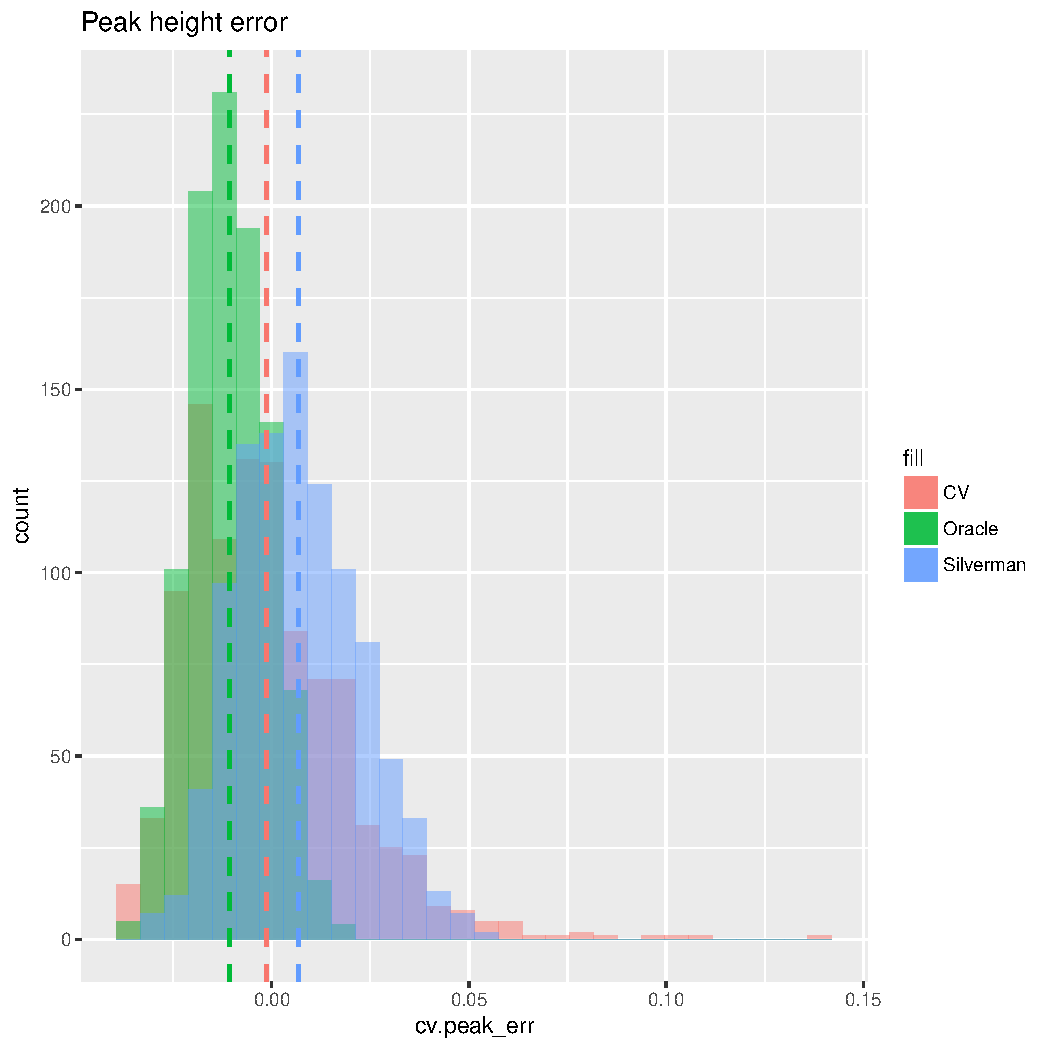
\includegraphics[width=\textwidth]{output/peak-height-histogram}
        \subcaption{Peak height error}
        \label{fig:peaks:unif_100_1.0_1h:height}
    \end{subfigure}
    \caption[Peak accuracy: Single-peak of 100 on uniform population]{Peak accuracy measure densities for a single-peak intensity with \glsentryname{spread} of 1.0 and \glsentryname{factor} of 100 on a uniform population. Vertical lines indicate the mean values of the simulations.}
    \label{fig:peaks:unif_100_1.0_1h}
\end{figure}

%%%%%%%%%%%%%%%%%%%%%%%%%%%%%%%%%%%%%%%%%%%%%%%%%
% Centroids - unif_100_1.0_1h
%%%%%%%%%%%%%%%%%%%%%%%%%%%%%%%%%%%%%%%%%%%%%%%%%
\begin{figure}[htbp]
    \centering
    \begin{subfigure}[b]{0.45\textwidth}
        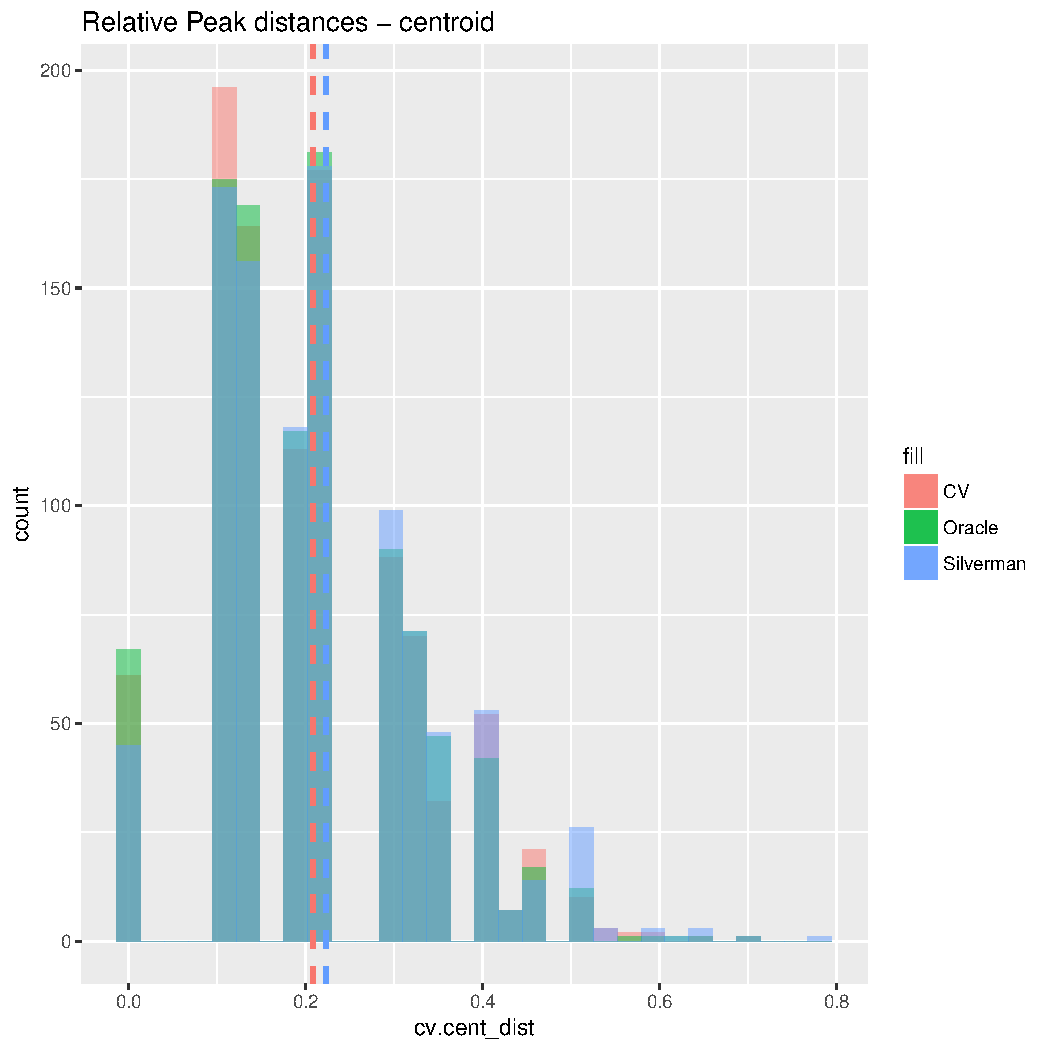
\includegraphics[width=\textwidth]{output/centroid-dist-histogram}
        \subcaption{Centroid peak distance from truth}
    \end{subfigure}
    \begin{subfigure}[b]{0.45\textwidth}
        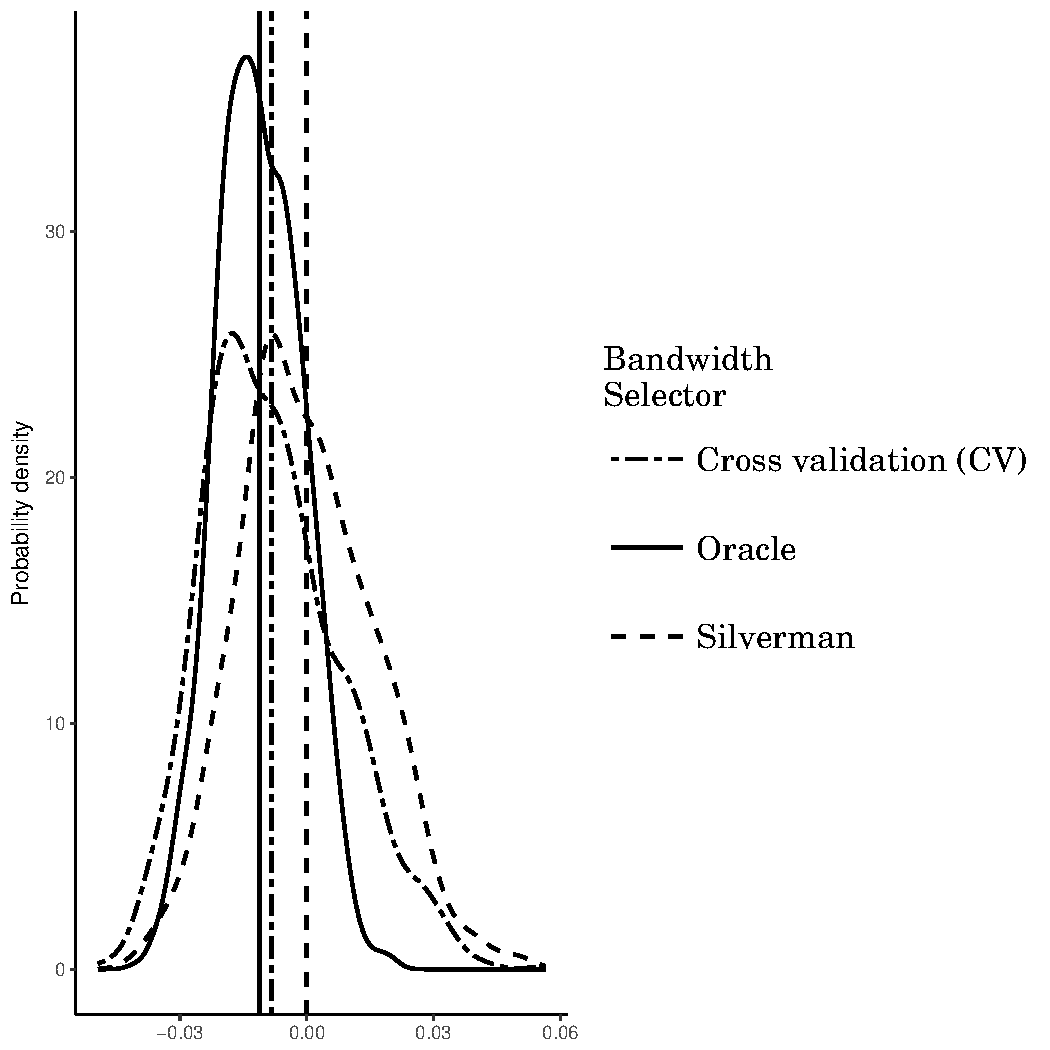
\includegraphics[width=\textwidth]{output/centroid-height-histogram}
        \subcaption{Centroid peak height error}
    \end{subfigure}
    \caption[Centroid accuracy: Single-peak of 100 on uniform population]{Peak accuracy measures densitiesu sing centroid technique for a single-peak intensity with \glsentryname{spread} of 1.0 and \glsentryname{factor} of 100 on a uniform population. Vertical lines indicate the mean values of the simulations.}
    \label{fig:centroids:unif_100_1.0_1h}
\end{figure}

For both of the peak distance errors (\cref{fig:peaks:unif_100_1.0_1h:dist}) and peak height errors (\cref{fig:peaks:unif_100_1.0_1h:height}) of this experiment,
we see the \gls{cv} bandwidth selection outperforms the \gls{silverman} rule of thumb, and that the \gls{oracle} seems to outperform them both.
In fact, the \gls{peak bias}, which we estimate using the mean \gls{peak error},
is positive for \gls{silverman}.
This indicates a tendency towards undersmoothing.
We note that all three of bandwidth selection techniques are designed to minimize \gls{mise}.
We also note the multi-modal peak distance distributions.
We believe this is an artifact of the experimental design,
since our estimate of the peak will always be at one of a fixed, discrete number of points on a grid in the study area.

In \cref{fig:centroids:unif_100_1.0_1h} we see the distributions of \gls{peak error} and \gls{peak drift} using the centroid estimation technique.
We note that the scales of both types of error are markedly improved.
That is, the centroid technique improves both the estimated location and estimated height of the peak.

%%%%%%%%%%%%%%%%%%%%%%%%%%%%%%%%%%%%%%%%%%%%%%%%%
% Bandwidths - unif_100_1.0_1h
%%%%%%%%%%%%%%%%%%%%%%%%%%%%%%%%%%%%%%%%%%%%%%%%%
\begin{figure}[htbp]
    \centering
    \begin{subfigure}[t]{0.45\textwidth}
        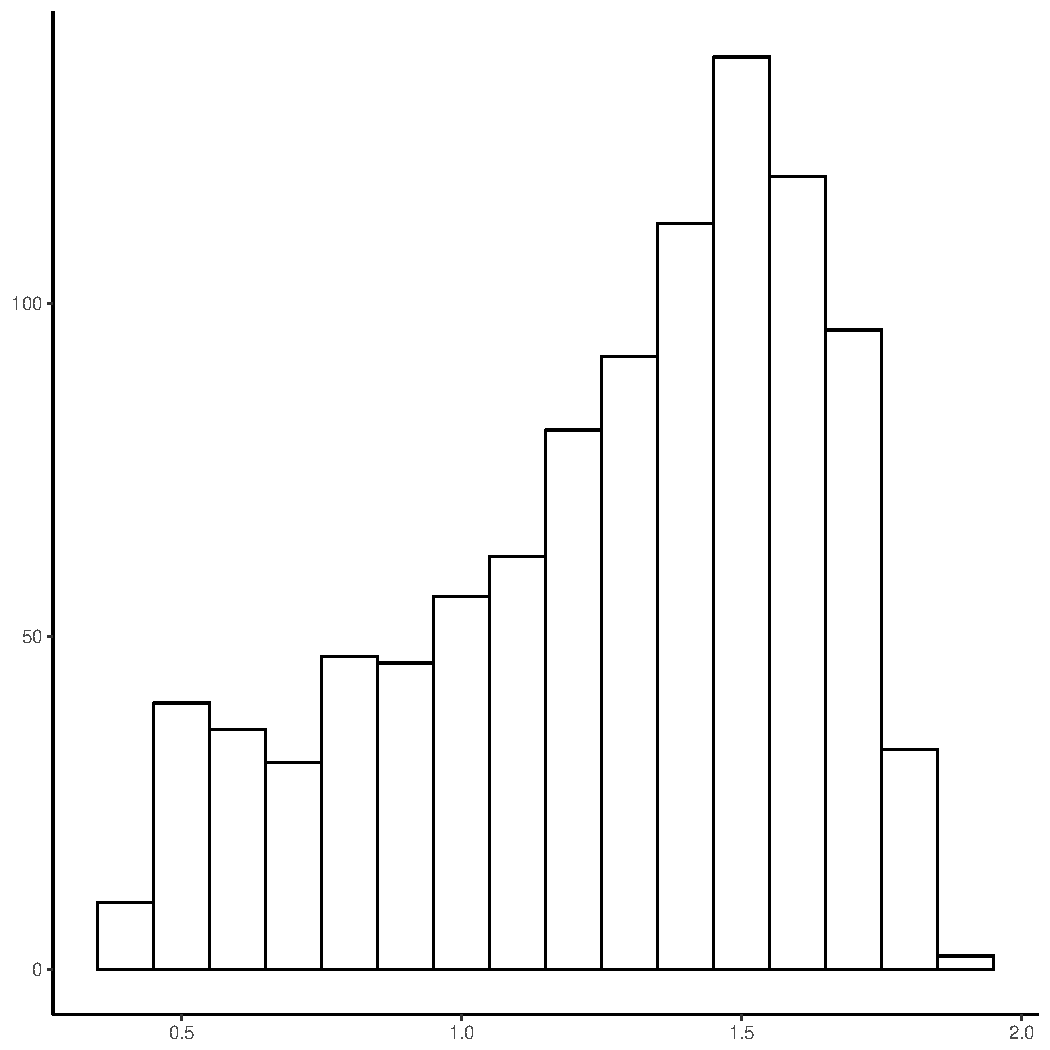
\includegraphics[width=\textwidth]{output/bandwidths-x1}
        \subcaption{CV Bandwidths - $x_1$}
        \label{fig:bandwidths:unif_100_1.0_1h:x1}
    \end{subfigure}
    \begin{subfigure}[t]{0.45\textwidth}
        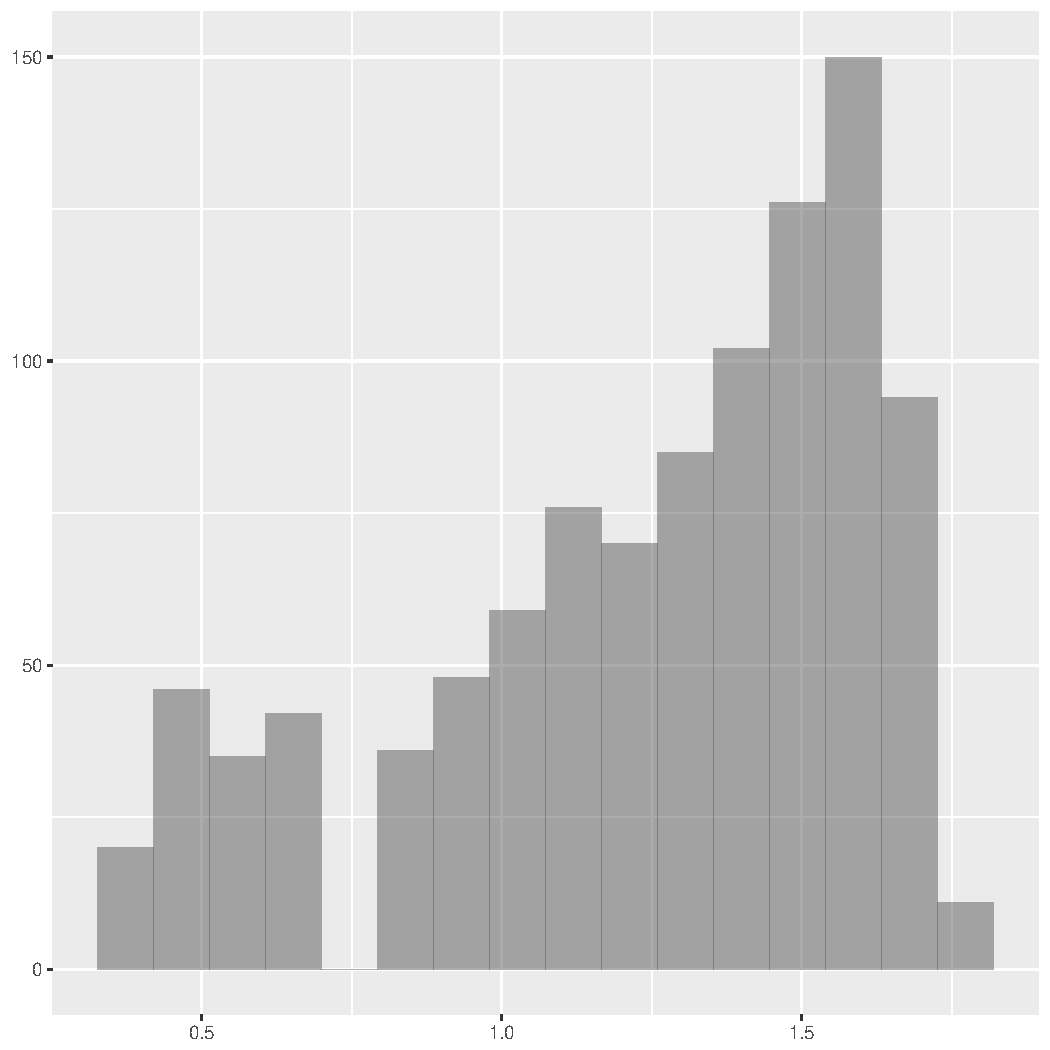
\includegraphics[width=\textwidth]{output/bandwidths-x2}
        \subcaption{CV Bandwidths - $x_2$}
        \label{fig:bandwidths:unif_100_1.0_1h:x2}
    \end{subfigure}

    \begin{subfigure}[t]{0.45\textwidth}
        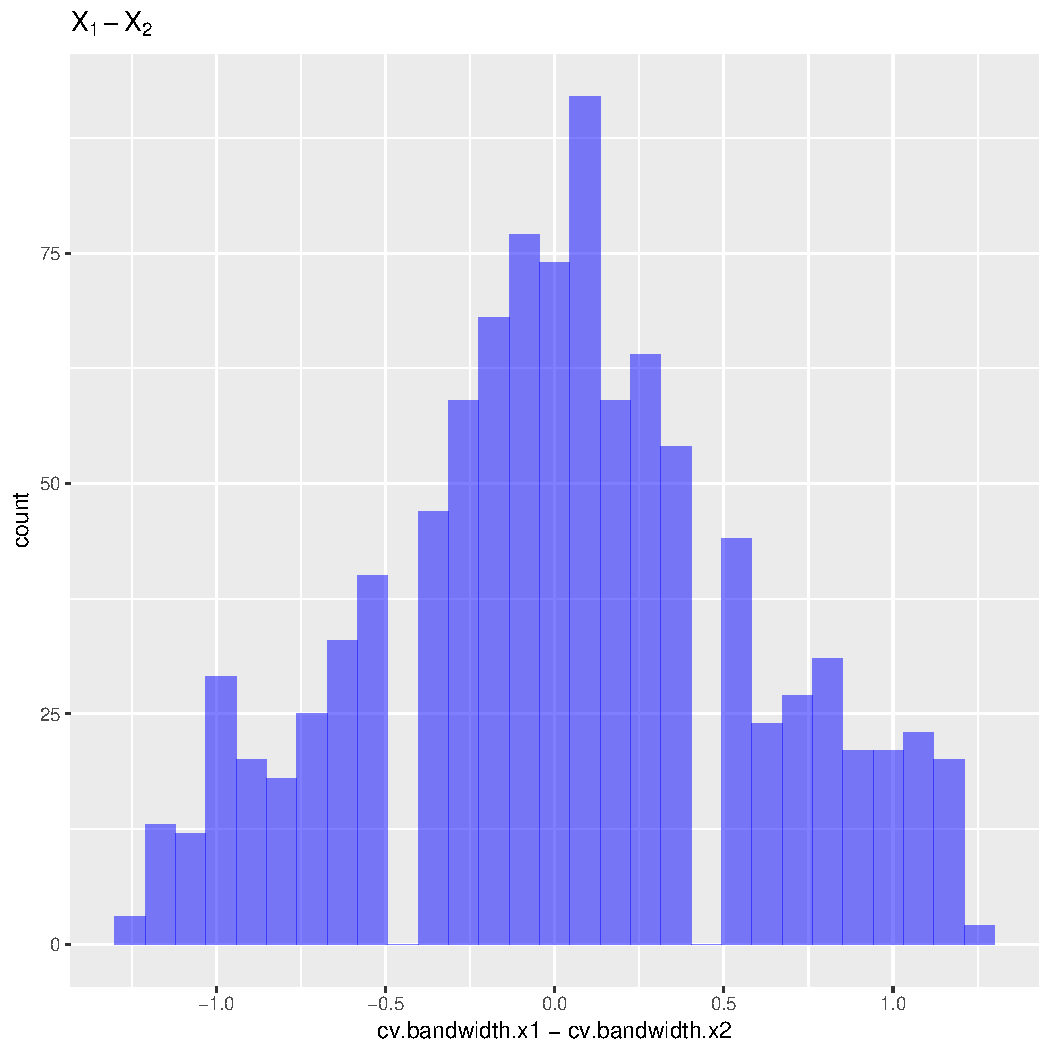
\includegraphics[width=\textwidth]{output/bandwidths-difference}
        \subcaption{Difference between $x_1$ and $x_2$ bandwidths}
        \label{fig:bandwidths:unif_100_1.0_1h:diff}
    \end{subfigure}
    \begin{subfigure}[t]{0.45\textwidth}
        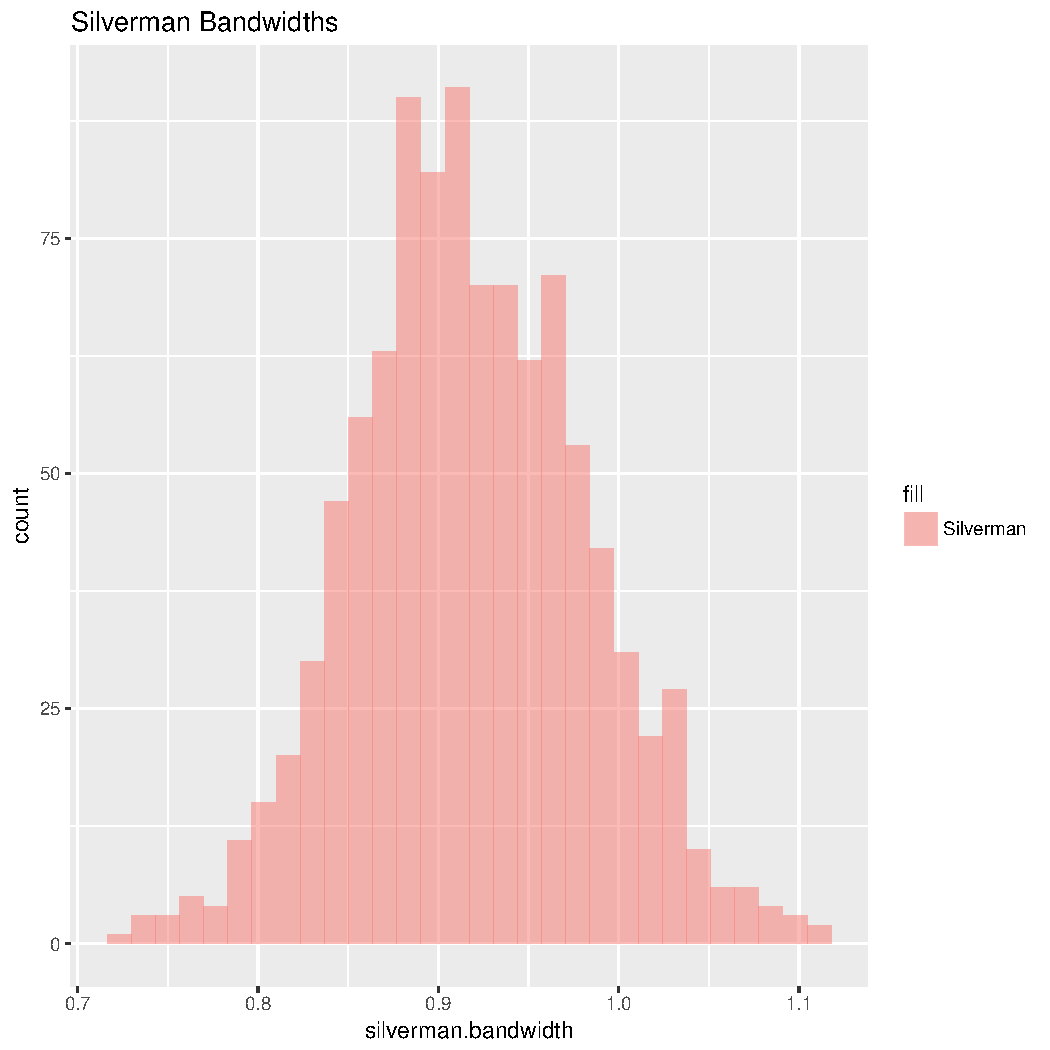
\includegraphics[width=\textwidth]{output/bandwidths-silverman}
        \subcaption{Silverman Bandwidths}
        \label{fig:bandwidths:unif_100_1.0_1h:silverman}
    \end{subfigure}
    \caption[Bandwidths: Single-peak of 100 on uniform population]{\glsentryname{cv} bandwidths: $x_1$, $x_2$ and difference and \glsentryname{silverman} bandwidth histograms for  a single-peak intensity with \glsentryname{spread} of 1.0 and \glsentryname{factor} of 100 on a uniform population}
    \label{fig:bandwidths:unif_100_1.0_1h}
\end{figure}

The bandwidths selected by \gls{cv} were allowed to vary in the $x_1$ and $x_2$ directions.
In \cref{fig:bandwidths:unif_100_1.0_1h:x1,fig:bandwidths:unif_100_1.0_1h:x2} we see that the distributions of these bandwidths observed in this experiment are quite similar,
while \cref{fig:bandwidths:unif_100_1.0_1h:diff} shows that they often differ significantly in the indidual realizations.
The distribution of the \gls{silverman} selected bandwidths is quite much more symmetric, and has a lower mean value (\cref{fig:bandwidths:unif_100_1.0_1h:silverman}).

% Restore graphics and input path
\graphicspath{{./}}
\makeatletter
\def\input@path{{./}}
\makeatother

%%%%%%%%%%%%%%%%%%%%%%%%%%%%%%%%%%%%%%%%%%%%%%%%%%%%%%%%%%%%%%%%%%%%%%%%%%%%%%
%%
%% Section: Effect of number of incidents with fixed population
%%
%%%%%%%%%%%%%%%%%%%%%%%%%%%%%%%%%%%%%%%%%%%%%%%%%%%%%%%%%%%%%%%%%%%%%%%%%%%%%%
\section[Effect of number of incidents with fixed population]
    {Effect of \glsentryname{factor} for a fixed, uniform population of 10,000 and single peak with \glsentryname{spread} 1.0}
\label{sec:results:number_of_incidents}

%%%%%%%%%%%%%%%%%%%%%%%%%%%%%%%%%%%%%%%%%%%%%%%%%
% Parameter table - expected number of incidents
%%%%%%%%%%%%%%%%%%%%%%%%%%%%%%%%%%%%%%%%%%%%%%%%%
\begin{table}[htbp]
    \centering
    \begin{tabular}{ll}
        \toprule
        Parameter & Value \\
        \midrule
        Population size & 10,000 \\
        Population \glsentryname{spread} & uniform \\
        Population center & uniform \\
        \Glsentryname{factor} & 50, 100, 200, 500, 1,000 \\
        Incident \glsentryname{spread} & 1.0 \\
        Incident center & (0,0) \\
        \bottomrule
    \end{tabular}
    \caption[Effect of \glsentryname{factor} with fixed population]
        {Experimental parameter values varying \glsentryname{factor} for a fixed, uniform population of 10,000 and single peak with spread 1.0}
    \label{tab:params:results:number_of_incidents}
\end{table}

In this section we examine and compare the results of five experiments in which we vary the \glspl{factor}
of a single-peak risk function.
The unknown information that one is trying to discover, is the risk of a person catching a specific disease over a defined time period.
This is analogous to a real-world researcher combining the several years worth of incident data from the same population.
Our question is, will this lead to more accurate results for the \gls{dkd}?
We keep the population size constant at 10,000, distributed uniformly throughout the study area.
The risk function for each of the five experiments has a single peak,
centered at the origin,
with a \gls{spread} of 1.0.
The \glspl{factor} used in the experiments in this section were 50, 100, 200, 500, and 1,000.
The full set of accuracy measures for these cases can be found in \cref{tab:mean_error_rates:unif_50_1.0_1h,tab:mean_error_rates:unif_100_1.0_1h,tab:mean_error_rates:unif_200_1.0_1h,tab:mean_error_rates:unif_500_1.0_1h,tab:mean_error_rates:unif_1000_1.0_1h} in \autoref{ch:results_tables}.
We note that as in \cref{sec:results:unif_100_1.0_1h}, the \gls{peak bias} values were positive for the \gls{silverman} bandwidth based estimates.
\autoref{fig:one_sample:unif_NCases_1h} shows how one realization of incidents, distributed over the population, for sample sizes of 100 and 500.

%%%%%%%%%%%%%%%%%%%%%%%%%%%%%%%%%%%%%%%%%%%%%%%%%
% Examples showing factorS
%%%%%%%%%%%%%%%%%%%%%%%%%%%%%%%%%%%%%%%%%%%%%%%%%
\begin{figure}[htbp]
    \centering
    \begin{subfigure}{0.45\textwidth}
        \includegraphics[width=\textwidth]{results/unif_100_1.0_1h/output/population_and_incidents_scatter}
        \caption{100 incidents}
    \end{subfigure}
    \begin{subfigure}{0.45\textwidth}
        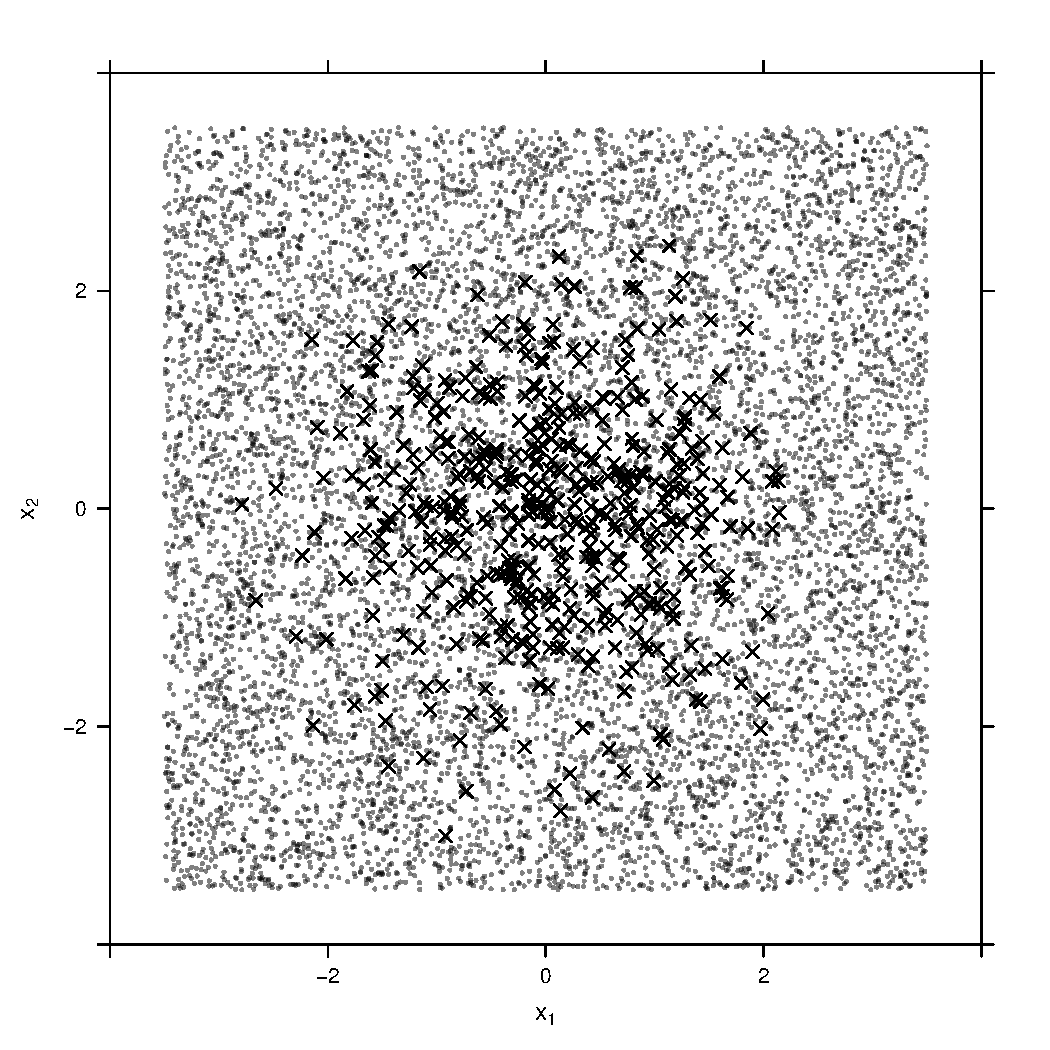
\includegraphics[width=\textwidth]{results/unif_500_1.0_1h/output/population_and_incidents_scatter}
        \caption{500 incidents}
    \end{subfigure}
        \caption{A single realization of different \glspl{factor} from a single-peak risk on a uniform population}
        \label{fig:one_sample:unif_NCases_1h}
\end{figure}

According to the theory developed in \cref{sec:theory:bandwidth},
the bandwidth should decrease as the \textit{observed} sample size increases according to the formula

\begin{equation}
    \label{eq:h_opt}
    \gls{h_opt} = O(n^{-\frac{1}{6}}) \text{.}
\end{equation}

\Cref{tab:results:bandwidth_vs_mu} compares the selected bandwidths and \gls{nmise} obtained for different \glspl{factor},
since this is the variable which we control.
We observe that all of the bandwidths decrease as \gls{mu} increases.
When there is a power relationship as in \cref{eq:h_opt} above, we can take the logarithm of both variables to produce a linear relationship.
The slope of the line in the log-log equation is equal to the power of the original equation.
\Cref{fig:results:bandwidth_by_incidents} shows log-log plots of the observed bandwidths that were obtained by the various selection mechanisms.
We have fit a line to each plot to show the linear relationship in the log-log equations, and hence the power relationship between the bandwidths selected by the different mechanisms and the sample size, represented by \gls{factor}.
The observed values for the power of $n$ as represented by $N_I$ are shown in \cref{tab:results:bandwidth_alpha_by_selector}.

%latex.default(df, file = "h_per_mu.tex", title = "h_per_mu",     where = "htbp", label = "tab:results:bandwidth_vs_mu", rowname = NULL,     booktabs = TRUE, cgroup = c("", "Mean Bandwidths", "NMISE"),     n.cgroup = c(1, 5, 3), colheads = c("$N_I$", "$h_{o1}$",         "$h_{o2}$", "$h_{s}$", "$h_{cv1}$", "$h_{cv2}$", "Oracle",         "Silverman", "CV"), cdec = c(0, rep(1, 5), rep(3, 3)),     caption.loc = "bottom", caption = "Bandwidth and accuracy by expected number of incidents for uniform population of 10,000 with single-peak risk function, spread of 1.0. The NMISE values are scaled by $10^9$.",     caption.lot = "Bandwidth and accuracy by expected number of incidents")%
\begin{table}[htbp]
\begin{center}
\begin{tabular}{rcrrrrrcrrr}
\toprule
\multicolumn{1}{c}{\bfseries }&\multicolumn{1}{c}{\bfseries }&\multicolumn{5}{c}{\bfseries Mean Bandwidths}&\multicolumn{1}{c}{\bfseries }&\multicolumn{3}{c}{\bfseries NMISE}\tabularnewline
\cline{3-7} \cline{9-11}
\multicolumn{1}{c}{$N_I$}&\multicolumn{1}{c}{}&\multicolumn{1}{c}{$h_{o1}$}&\multicolumn{1}{c}{$h_{o2}$}&\multicolumn{1}{c}{$h_{s}$}&\multicolumn{1}{c}{$h_{cv1}$}&\multicolumn{1}{c}{$h_{cv2}$}&\multicolumn{1}{c}{}&\multicolumn{1}{c}{Oracle}&\multicolumn{1}{c}{Silverman}&\multicolumn{1}{c}{CV}\tabularnewline
\midrule
$  50$&&$1.5$&$1.5$&$1.0$&$1.4$&$1.4$&&$3.541$&$5.718$&$5.438$\tabularnewline
$ 100$&&$1.3$&$1.4$&$0.9$&$1.3$&$1.2$&&$2.220$&$3.526$&$3.398$\tabularnewline
$ 200$&&$1.2$&$1.2$&$0.8$&$1.1$&$1.1$&&$1.324$&$2.085$&$1.988$\tabularnewline
$ 500$&&$1.1$&$1.0$&$0.7$&$0.9$&$0.9$&&$0.679$&$1.067$&$0.959$\tabularnewline
$1000$&&$0.9$&$0.9$&$0.6$&$0.9$&$0.8$&&$0.382$&$0.621$&$0.541$\tabularnewline
\bottomrule
\end{tabular}
\caption[Bandwidth and accuracy by expected number of incidents]{Bandwidth and accuracy by expected number of incidents for uniform population of 10,000 with single-peak risk function, spread of 1.0. The NMISE values are scaled by $10^9$.\label{tab:results:bandwidth_vs_mu}}\end{center}
\end{table}


%latex.default(df.alpha, file = "alpha_by_selector.tex", title = "alpha_by_selector",     where = "htbp", label = "tab:results:bandwidth_alpha_by_selector",     rowname = NULL, cdec = c(0, 3), caption.loc = "bottom", caption = "Bandwidth onvergence rate $\\alpha$ of for different bandwidth selectors for a single-peak risk function with spread of 1.0 on a uniform population of 10,000.",     caption.lot = "Bandwidth convergence rate of bandwidth selectors")%
\begin{table}[htbp]
\begin{center}
\begin{tabular}{lr}
\hline\hline
\multicolumn{1}{c}{Selector}&\multicolumn{1}{c}{Slope}\tabularnewline
\hline
Oracle Bandwidth $x_1$&$-0.156$\tabularnewline
Oracle Bandwidth $x_1$&$-0.179$\tabularnewline
Silverman&$-0.167$\tabularnewline
CV Bandwidth $x_1$&$-0.171$\tabularnewline
CV Bandwidth $x_2$&$-0.205$\tabularnewline
Theory&$-0.167$\tabularnewline
\hline
\end{tabular}
\caption[Bandwidth convergence rate of bandwidth selectors]{Bandwidth onvergence rate $\alpha$ of for different bandwidth selectors for a single-peak risk function with spread of 1.0 on a uniform population of 10,000.\label{tab:results:bandwidth_alpha_by_selector}}\end{center}
\end{table}


%%%%%%%%%%%%%%%%%%%%%%%%%%%%%%%%%%%%%%%%%%%%%%%%%
% Selected bandwidty by factor
%%%%%%%%%%%%%%%%%%%%%%%%%%%%%%%%%%%%%%%%%%%%%%%%%
\begin{figure}[htbp]
    \centering
    \begin{subfigure}[t]{0.195\textwidth}
        \centering
        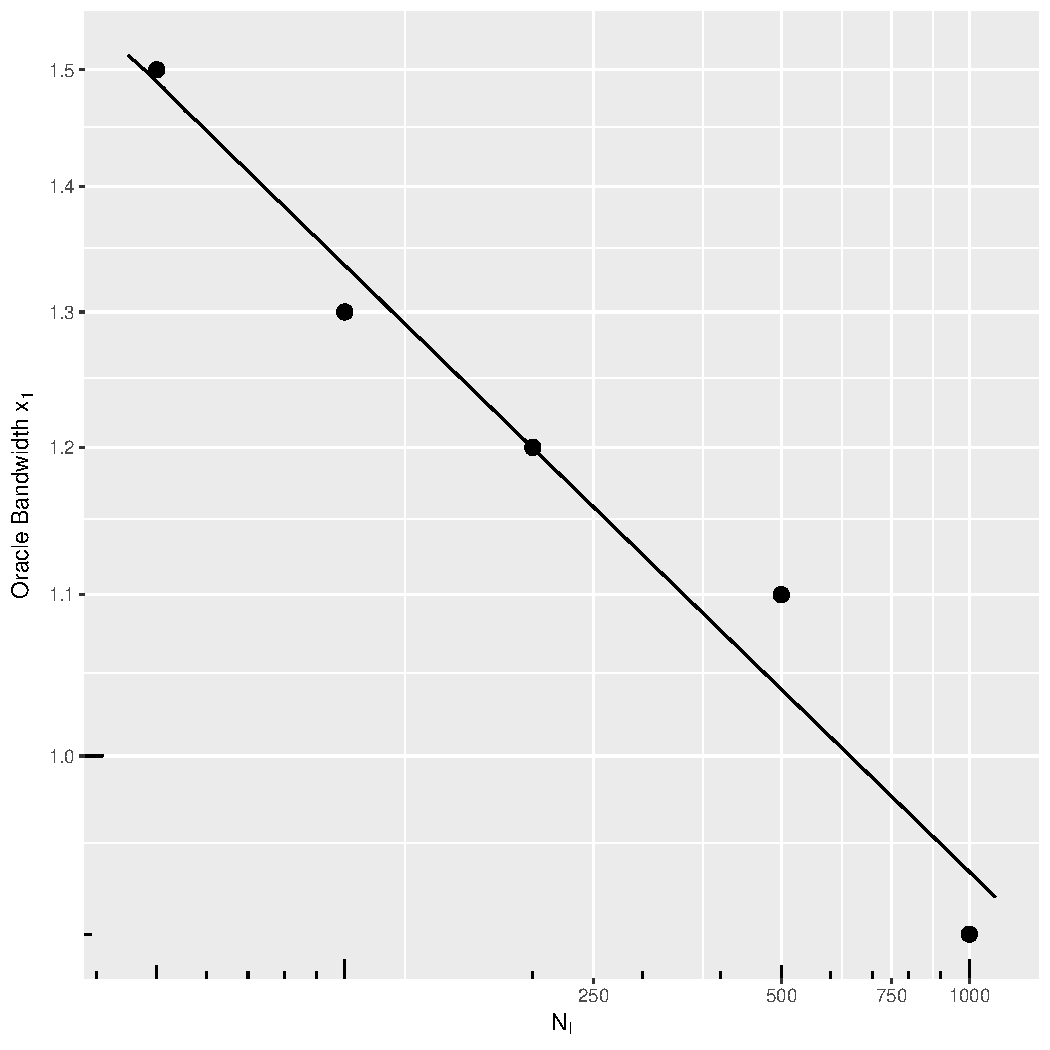
\includegraphics[width=\textwidth]{results/by_h_per_mu/oracle_bandwidth_x1_vs_mu.pdf}
        \subcaption{Oracle bandwidth in $x_1$ direction by \glsentryname{factor}}
    \end{subfigure}
    \begin{subfigure}[t]{0.195\textwidth}
        \centering
        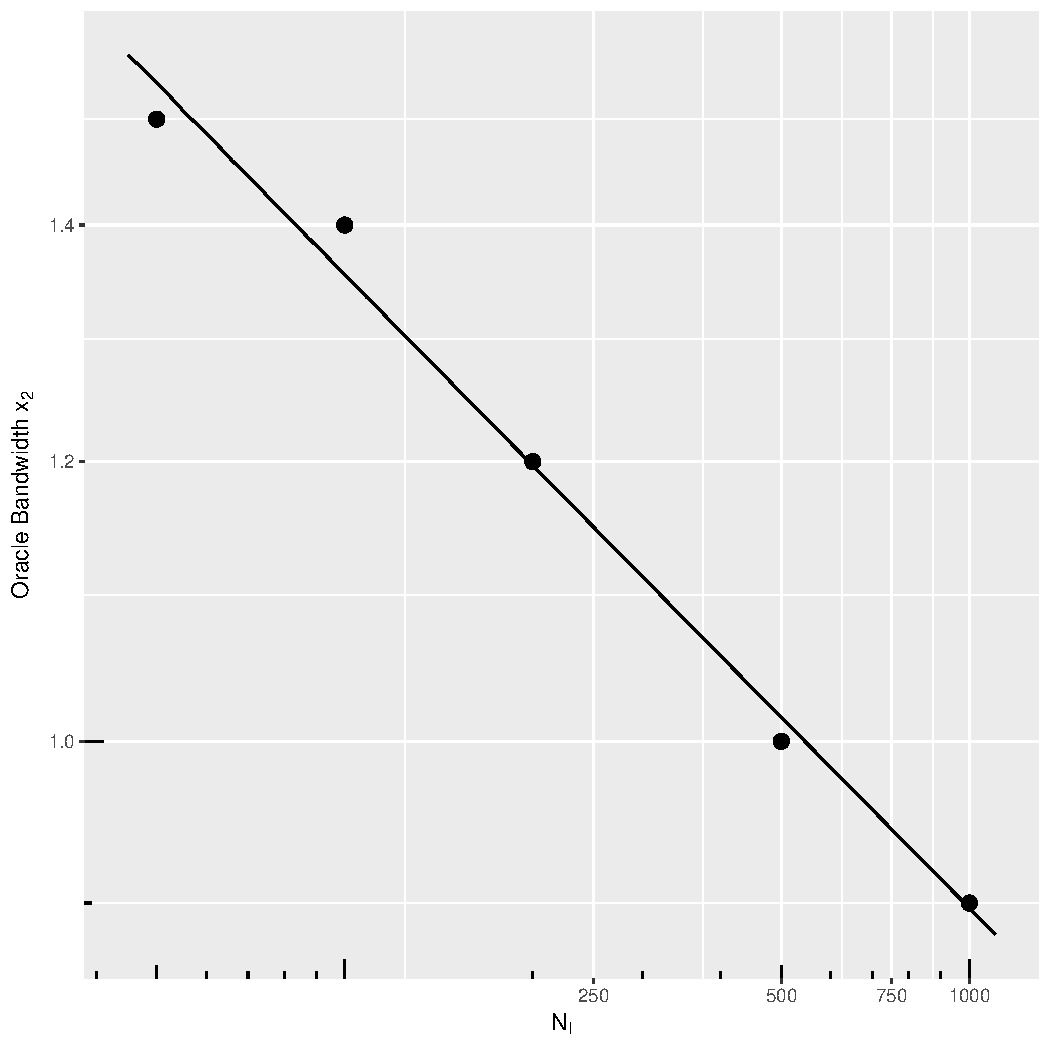
\includegraphics[width=\textwidth]{results/by_h_per_mu/oracle_bandwidth_x2_vs_mu.pdf}
        \subcaption{Oracle bandwidth in $x_2$ direction by \glsentryname{factor}}
    \end{subfigure}
    \begin{subfigure}[t]{0.195\textwidth}
        \centering
        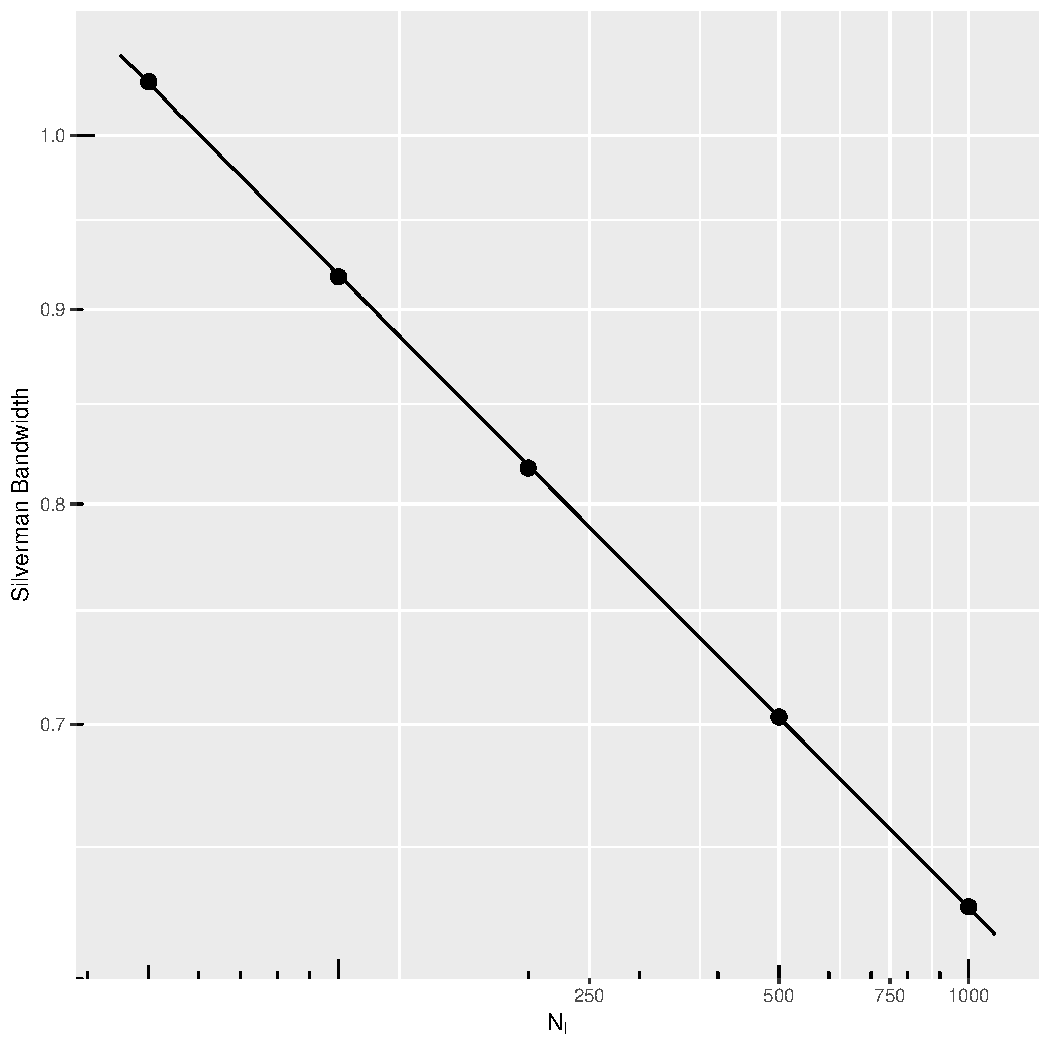
\includegraphics[width=\textwidth]{results/by_h_per_mu/silverman_bandwidth_vs_mu.pdf}
        \subcaption{Mean Silverman bandwidth by \glsentryname{factor}}
    \end{subfigure}
    \begin{subfigure}[t]{0.195\textwidth}
        \centering
        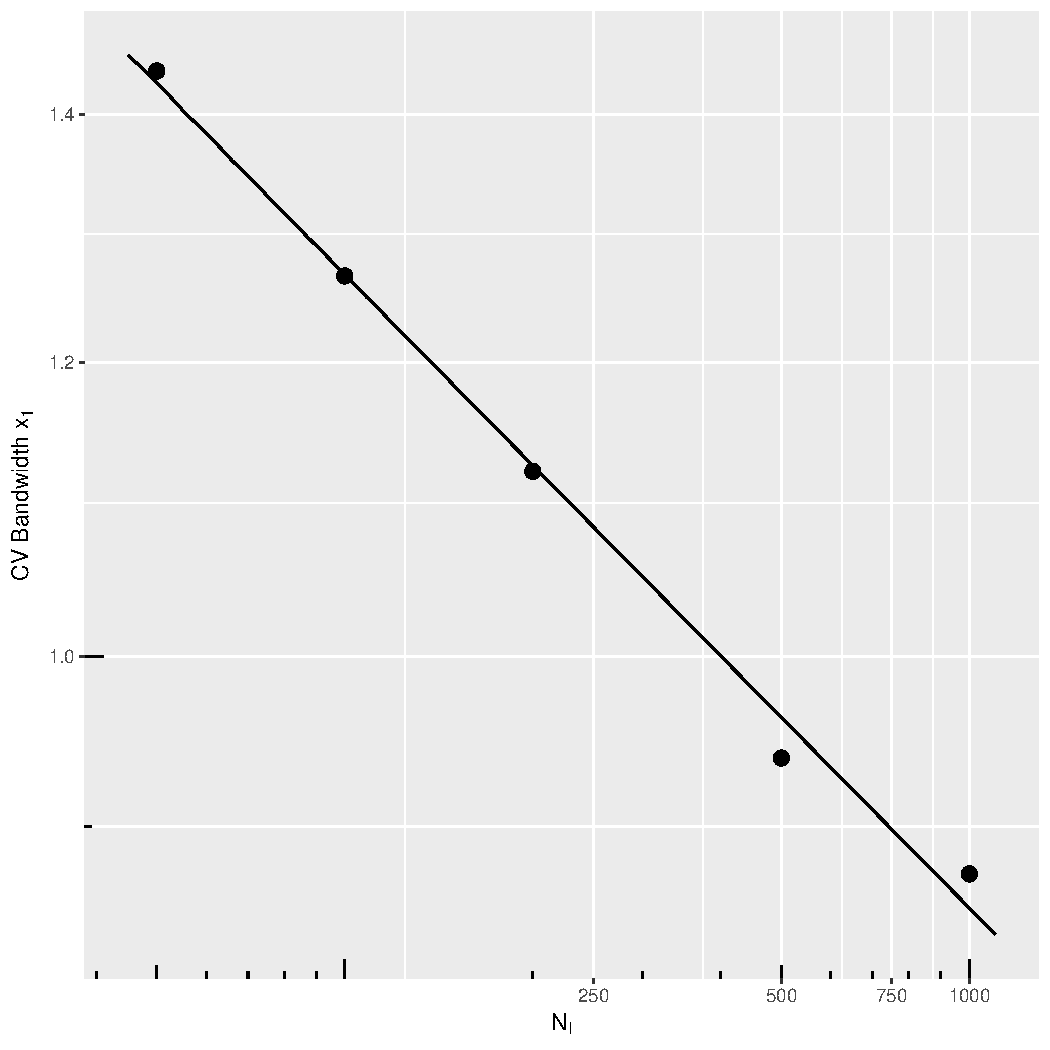
\includegraphics[width=\textwidth]{results/by_h_per_mu/cv_bandwidth_x1_vs_mu.pdf}
        \subcaption{Mean CV bandwidth in $x_1$ direction by \glsentryname{factor}}
    \end{subfigure}
    \begin{subfigure}[t]{0.195\textwidth}
        \centering
        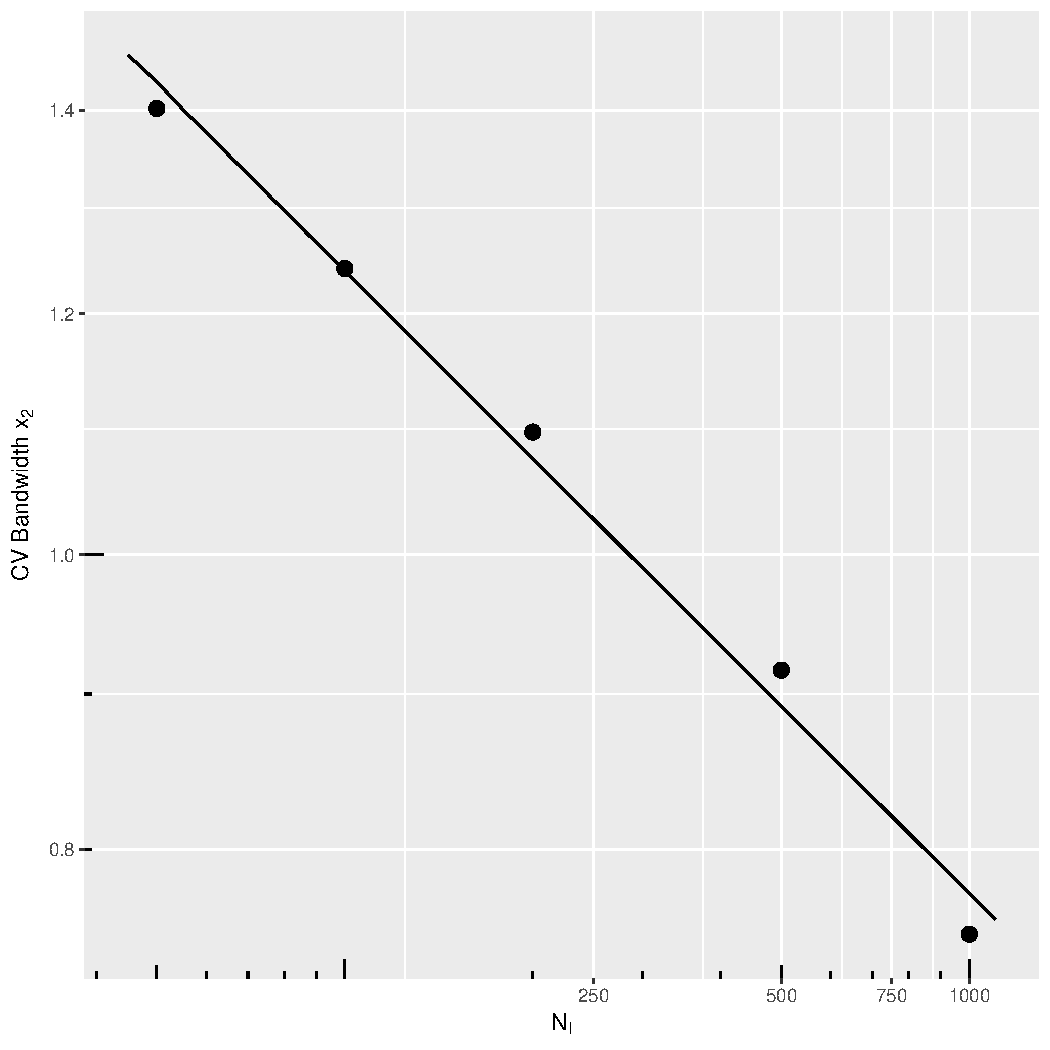
\includegraphics[width=\textwidth]{results/by_h_per_mu/cv_bandwidth_x2_vs_mu.pdf}
        \subcaption{Mean CV bandwidth in $x_2$ direction by \glsentryname{factor}}
    \end{subfigure}
    \caption[Selected bandwidth by \glsentryname{factor}]
        {Log-log plot of selected bandwidth by \glsentryname{factor} for different bandwidth selectors.
        The slope of the log-log plot indicates the power of $n$ in the convergence rate.}
    \label{fig:results:bandwidth_by_incidents}    
\end{figure}

%%%%%%%%%%%%%%%%%%%%%%%%%%%%%%%%%%%%%%%%%%%%%%%%%
% MISE by number of cases
%%%%%%%%%%%%%%%%%%%%%%%%%%%%%%%%%%%%%%%%%%%%%%%%%
\begin{figure}[htbp]
    \centering
    \begin{subfigure}[b]{0.24\textwidth}
        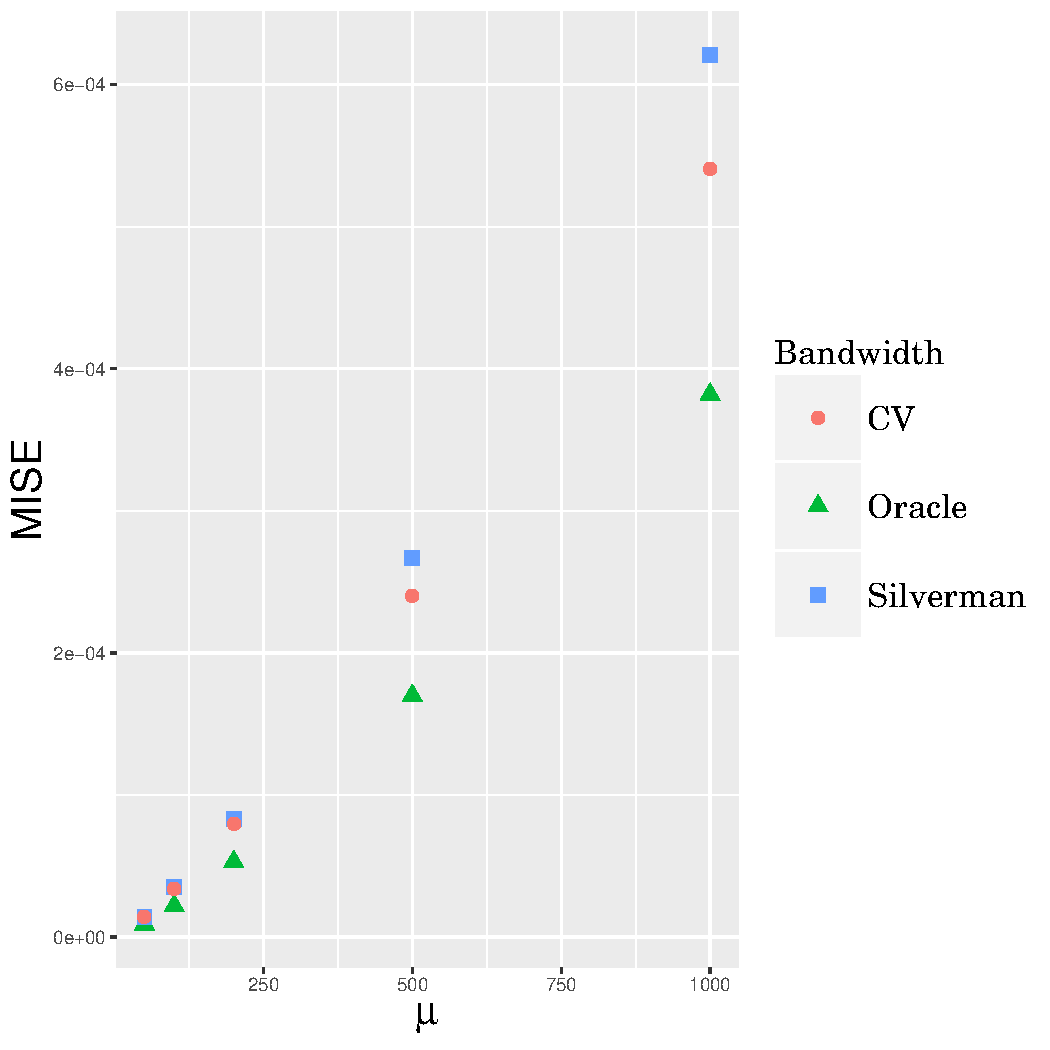
\includegraphics[width=\textwidth]{results/by_num_cases/MISE-vs-cases}
        \subcaption{\glsentryname{mise}}
        \label{fig:ise:unif_NCases_1h:mise}
    \end{subfigure}
    \begin{subfigure}[b]{0.24\textwidth}
        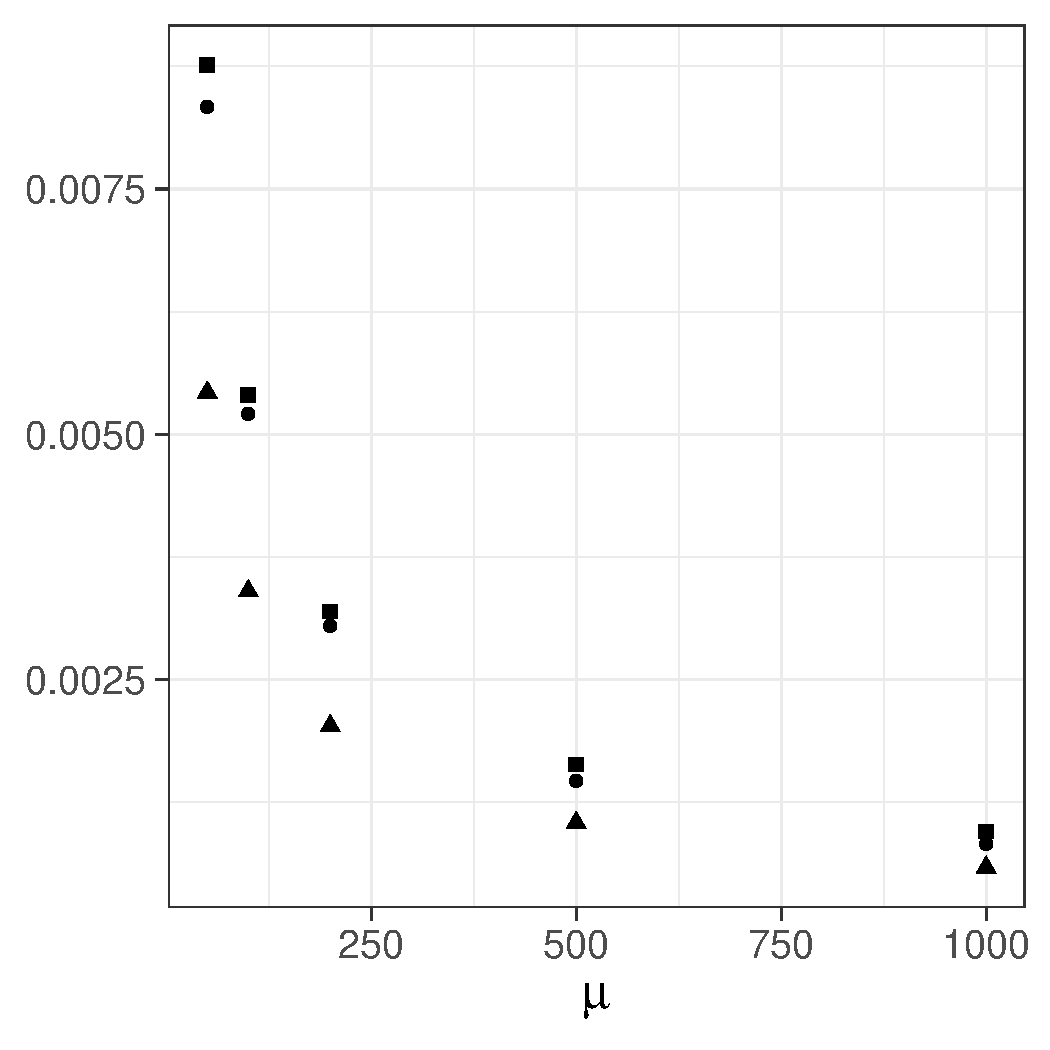
\includegraphics[width=\textwidth]{results/by_num_cases/RMISE-vs-cases}
        \subcaption{\glsentryname{rmise}}
        \label{fig:ise:unif_NCases_1h:rmise}
    \end{subfigure}
    \begin{subfigure}[b]{0.24\textwidth}
        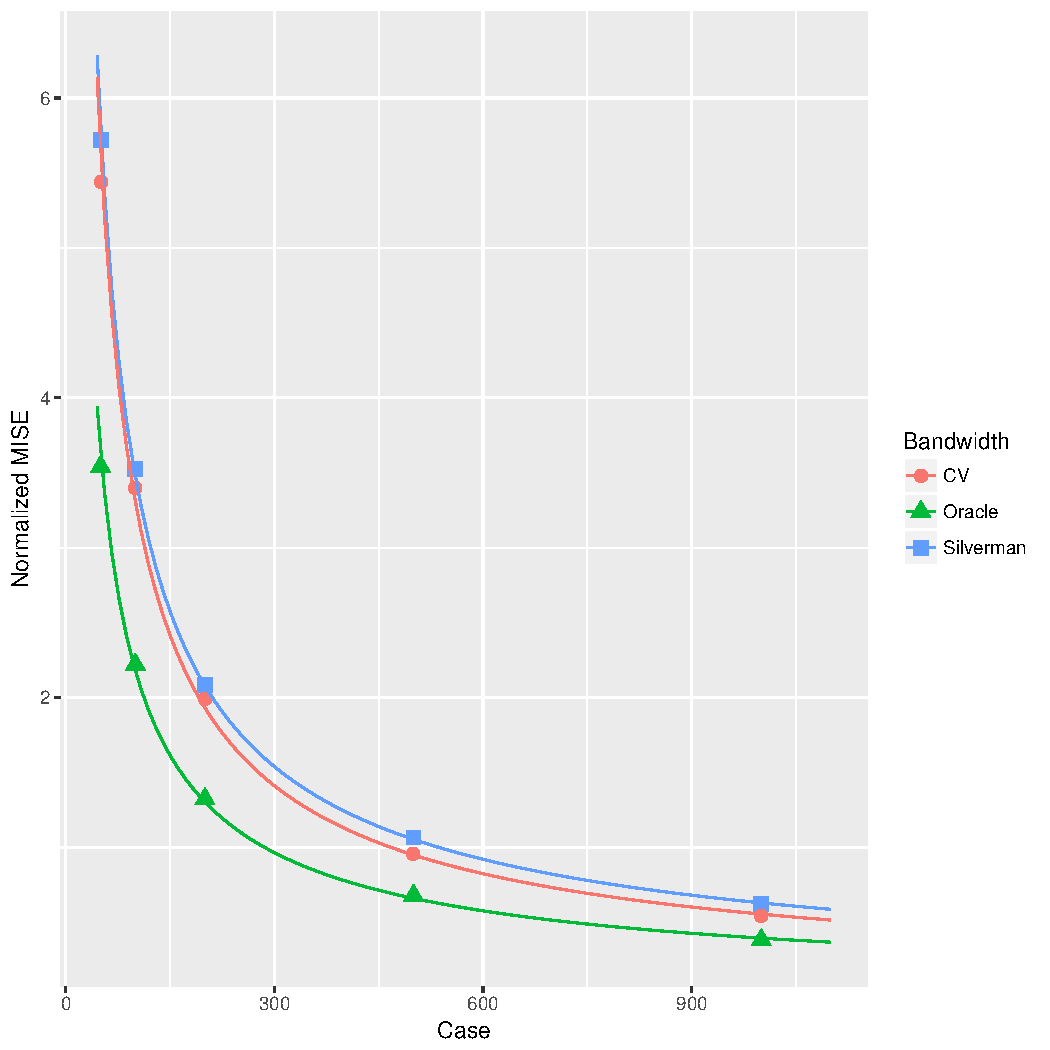
\includegraphics[width=\textwidth]{results/by_num_cases/NMISE-vs-cases}
        \subcaption{\glsentryname{nmise}}
        \label{fig:ise:unif_NCases_1h:nmise}
    \end{subfigure}
    \begin{subfigure}[b]{0.24\textwidth}
        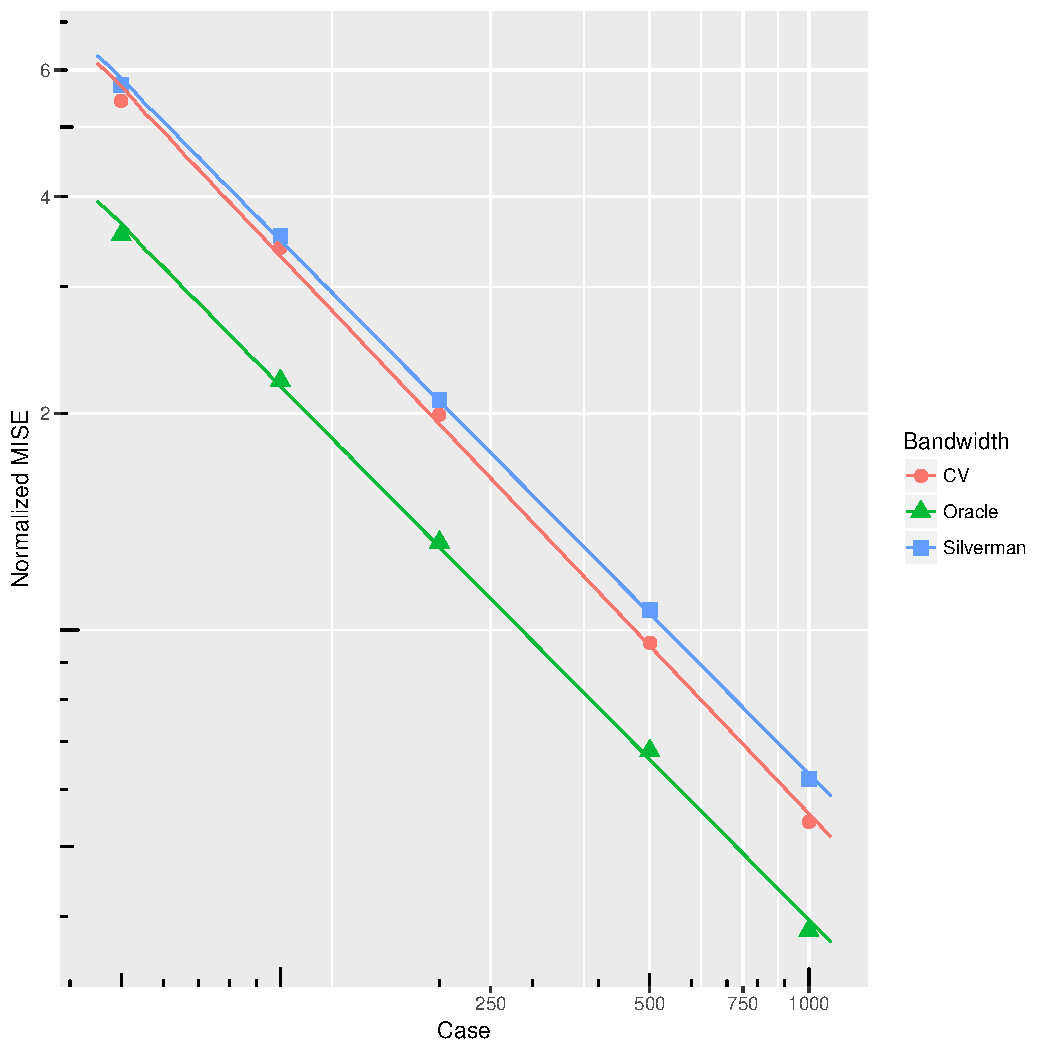
\includegraphics[width=\textwidth]{results/by_num_cases/NMISE-vs-cases-log-log}
        \subcaption{\glsentryname{nmise} log-log}
        \label{fig:ise:unif_NCases_1h:nmise_log_log}
    \end{subfigure}
    \caption[\glsentryname{mise}: by number of cases]{\glsentryname{mise} vs. number of cases}
    \label{fig:ise:unif_NCases_1h}
\end{figure}

\autoref{fig:ise:unif_NCases_1h} shows the effect of \gls{factor} on the \gls{mise}, \gls{rmise} and on \gls{nmise}:
\autoref{fig:ise:unif_NCases_1h:mise} shows how \gls{mise} increases with \gls{factor}.
One might expect the error to associated with estimating a function to \textit{decrease} as the \gls{factor} increases.
However, the \gls{factor} increases linearly with the intensity function value.
For example, double the number of incidents corresponds to an intensity of twice the value.
This makes comparing the \gls{mise} of estimates of intensity functions difficult,
as the errors will also rise in the same direction.
In order to facilitate the comparison of intensity functions that have different expected number of incidents,
we use the \gls{rmise}and \gls{nmise}.
\Cref{fig:ise:unif_NCases_1h:rmise,fig:ise:unif_NCases_1h:nmise} shows how \gls{rmise} and \gls{nmise} decreases with \gls{factor}.
To test if there is a power relationship between \gls{nmise} and \gls{factor},
we take the logarithms of each variable and fit a line.
\autoref{fig:ise:unif_NCases_1h:nmise_log_log} is a log-log graph,
showing the linear relationship between the logarithm of \gls{nmise} and the logarithm of the \gls{factor}.
This indicates a power relationship between \gls{nmise} and \gls{factor} for each bandwidth selection method is shown in \cref{tab:results:nmise_convergence_by_num_cases}.
They are all near to $-0.75$.

%latex.default(df.alpha, title = "nmise_convergence_table", where = "htbp",     label = "tab:results:nmise_convergence_by_num_cases", rowname = NULL,     booktabs = TRUE, cdec = c(0, 3), caption.loc = "bottom",     caption = "NMISE onvergence rate by number of cases for different bandwidth selectors for a single-peak risk function with spread of 1.0 on a uniform population of 10,000.",     caption.lot = "NMISE Convergence rate by number of cases for spread 1.0")%
\begin{table}[htbp]
\begin{center}
\begin{tabular}{lr}
\toprule
\multicolumn{1}{c}{Selector}&\multicolumn{1}{c}{Slope}\tabularnewline
\midrule
Oracle&$-0.742$\tabularnewline
Silverman&$-0.741$\tabularnewline
CV&$-0.775$\tabularnewline
\bottomrule
\end{tabular}
\caption[NMISE Convergence rate by number of cases for spread 1.0]{NMISE onvergence rate by number of cases for different bandwidth selectors for a single-peak risk function with spread of 1.0 on a uniform population of 10,000.\label{tab:results:nmise_convergence_by_num_cases}}\end{center}
\end{table}



%%%%%%%%%%%%%%%%%%%%%%%%%%%%%%%%%%%%%%%%%%%%%%%%%%%%%%%%%%%%%%%%%%%%%%%%%%%%%%
%%
%% Section: Effect of risk spread with fixed population
%%
%%%%%%%%%%%%%%%%%%%%%%%%%%%%%%%%%%%%%%%%%%%%%%%%%%%%%%%%%%%%%%%%%%%%%%%%%%%%%%
\section[Effect of risk spread with fixed population]
    {Effect of risk \glsentryname{spread} for a fixed, uniform population of 10,000 and single peak with \glsentryname{spread} 1.0}
\label{sec:results:spread}

%%%%%%%%%%%%%%%%%%%%%%%%%%%%%%%%%%%%%%%%%%%%%%%%%
% Parameter table - spread
%%%%%%%%%%%%%%%%%%%%%%%%%%%%%%%%%%%%%%%%%%%%%%%%%
\begin{table}[htbp]
    \centering
    \begin{tabular}{ll}
        \toprule
        Parameter & Value \\
        \midrule
        Population size & 10,000 \\
        Population \glsentryname{spread} & uniform \\
        Population center & uniform \\
        \Glsentryname{factor} & 100 \\
        Incident \glsentryname{spread} & 0.7, 1.0, 1.4, 2.0, 2.8 \\
        Incident center & (0,0) \\
        \bottomrule
    \end{tabular}
    \caption[Effect of spread with fixed population]
        {Experimental parameter values varying \glsentryname{spread} for a fixed, uniform population of 10,000 and single peak with \glsentryname{spread} 1.0}
    \label{tab:params:results:spread}
\end{table}

In this section we examine and compare the results of five experiments in which we vary the \gls{spread} \gls{sigma_i}
of a single-peak risk function.
The unknown information that one is trying to discover is, how far away from a source of disease risk is safe.
Our question is, under different \glspl{spread}, how accurate is the \gls{dkd}?
Differing \glspl{spread} are analogous to different levels of concentration of the risk of disease is in a specific location.
Another way to look at it is, is how quickly the risk dissipates in space as one moves further away from a single source of disease risk.
We keep the population size constant at 10,000, distributed uniformly throughout the study area.
The risk function for each of the five experiments has a single peak,
centered at the origin,
with a \gls{factor} of 100.
The values of \gls{sigma_i} used in the experiments in this section are 0.7, 1.0, 1.4, 2.0, and 2.8.
The full set of accuracy measures for these cases can be found in \autoref{tab:mean_error_rates:unif_100_0.7_1h}, \autoref{tab:mean_error_rates:unif_100_1.0_1h}, \autoref{tab:mean_error_rates:unif_100_1.4_1h}, \autoref{tab:mean_error_rates:unif_100_2.0_1h}, and \autoref{tab:mean_error_rates:unif_100_2.8_1h} in \autoref{ch:results_tables}.
We note that as in \cref{sec:results:unif_100_1.0_1h}, the \gls{peak bias} values were positive for the \gls{silverman} bandwidth based estimates.
\autoref{fig:one_sample:unif_Spreads_1h} shows how one realization of incidents, distributed over the population, for \glspl{spread} of 1.0 and 2.8.

%%%%%%%%%%%%%%%%%%%%%%%%%%%%%%%%%%%%%%%%%%%%%%%%%
% Examples showing incident spreads
%%%%%%%%%%%%%%%%%%%%%%%%%%%%%%%%%%%%%%%%%%%%%%%%%
\begin{figure}[htbp]
    \centering
    \begin{subfigure}{0.45\textwidth}
        \includegraphics[width=\textwidth]{results/unif_100_1.0_1h/output/population_and_incidents_scatter}
        \caption{\gls{sigma_i} = 1.0}
    \end{subfigure}
    \begin{subfigure}{0.45\textwidth}
        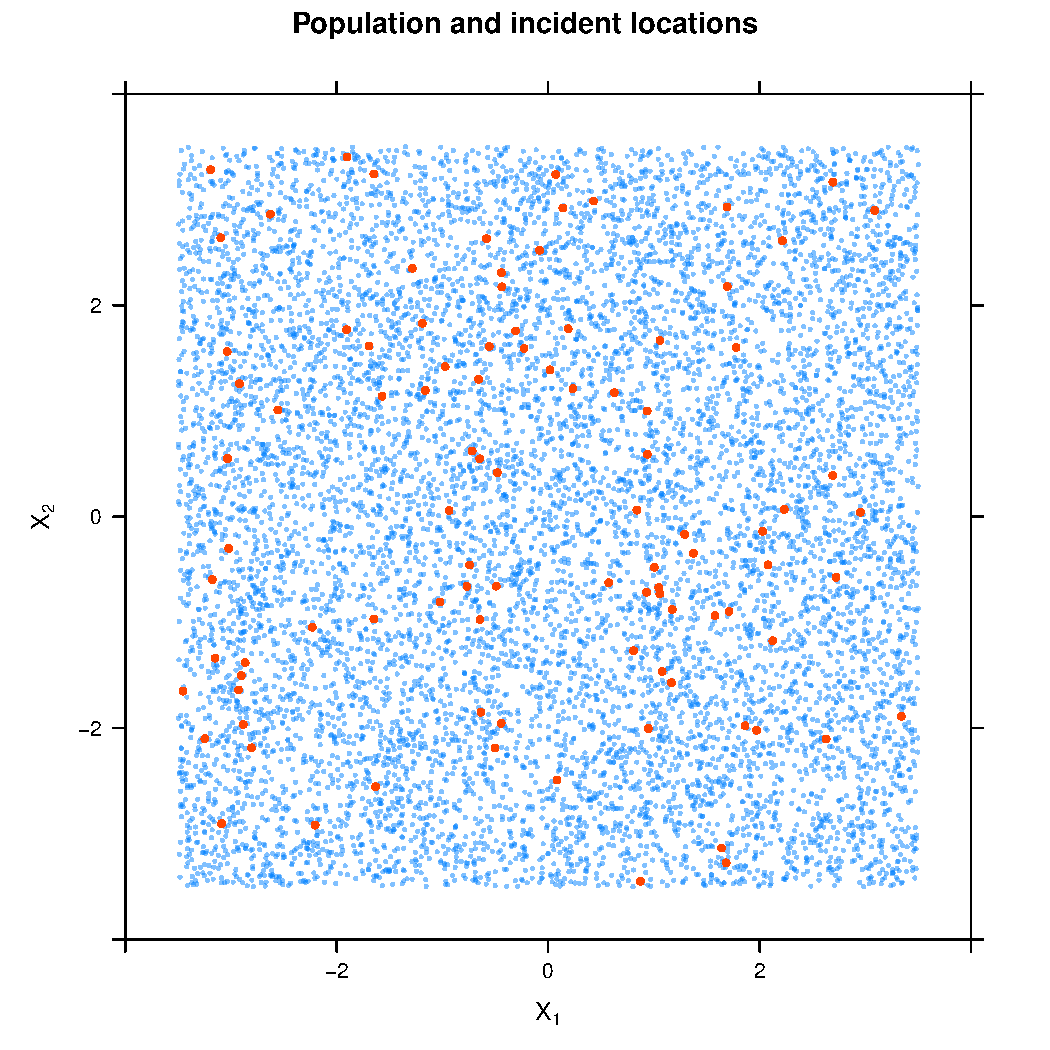
\includegraphics[width=\textwidth]{results/unif_100_2.8_1h/output/population_and_incidents_scatter}
        \caption{\gls{sigma_i} = 2.8}
    \end{subfigure}
    \caption[Examples showing incident spread]
        {A single realization of different incident \glspl{spread} from a single-peak risk on a uniform population}
    \label{fig:one_sample:unif_Spreads_1h}
\end{figure}

The effect of increasing \gls{spread} is that the peak of the risk function becomes less pronounced.
The incidents that are generated by the corresponding \gls{spp} are distributed more evenly and widely throughout the study area \gls{W},
as can be seen in \cref{fig:one_sample:unif_Spreads_1h}.
We observe the effect of varying \gls{sigma_i} on the selected bandwidths.
The \gls{oracle}, \gls{silverman}, and \gls{cv} bandwidths all increase as the spread increases, as can be seen in \cref{tab:results:bandwidth_vs_spread}.
This is to be expected, since smaller bandwidths result in decreased smoothing,
which is necessary when the true risk function varies more quickly as is the case with smaller \gls{sigma_i} values.
We note that the \gls{cv} selected bandwidths are closer to \gls{h_opt} as approximated by the \gls{oracle}, than are the \gls{silverman} bandwidths.

%latex.default(df, file = "h_per_spread.tex", title = "h_per_spread",     where = "htbp", label = "tab:results:bandwidth_vs_spread",     rowname = NULL, cgroup = c("", "Mean Bandwidths", "NMISE"),     n.cgroup = c(1, 5, 3), colheads = c("$\\sigma_i$", "$h_{o1}$",         "$h_{o2}$", "$h_{s}$", "$h_{cv1}$", "$h_{cv2}$", "Oracle",         "Silverman", "CV"), cdec = c(1, rep(1, 5), rep(3, 3)),     caption.loc = "bottom", caption = "Bandwidth and accuracy by spread for uniform population of 10,000 with single-peak risk function with expected number of incidents 100. The NMISE values are scaled by $10^9$.",     caption.lot = "Bandwidth and accuracy by spread of incidents")%
\begin{table}[htbp]
\begin{center}
\begin{tabular}{lcrrrrrcrrr}
\hline\hline
\multicolumn{1}{c}{\bfseries }&\multicolumn{1}{c}{\bfseries }&\multicolumn{5}{c}{\bfseries Mean Bandwidths}&\multicolumn{1}{c}{\bfseries }&\multicolumn{3}{c}{\bfseries NMISE}\tabularnewline
\cline{3-7} \cline{9-11}
\multicolumn{1}{c}{$\sigma_i$}&\multicolumn{1}{c}{}&\multicolumn{1}{c}{$h_{o1}$}&\multicolumn{1}{c}{$h_{o2}$}&\multicolumn{1}{c}{$h_{s}$}&\multicolumn{1}{c}{$h_{cv1}$}&\multicolumn{1}{c}{$h_{cv2}$}&\multicolumn{1}{c}{}&\multicolumn{1}{c}{Oracle}&\multicolumn{1}{c}{Silverman}&\multicolumn{1}{c}{CV}\tabularnewline
\hline
0.7&&$0.9$&$1.0$&$0.6$&$0.9$&$0.9$&&$4.151$&$6.976$&$6.667$\tabularnewline
1.0&&$1.3$&$1.4$&$0.9$&$1.3$&$1.2$&&$2.220$&$3.526$&$3.398$\tabularnewline
1.4&&$1.9$&$1.8$&$1.3$&$1.7$&$1.7$&&$1.163$&$1.869$&$1.637$\tabularnewline
2.0&&$2.5$&$2.6$&$1.6$&$2.1$&$2.1$&&$0.642$&$1.187$&$0.919$\tabularnewline
\hline
\end{tabular}
\caption[Bandwidth and accuracy by spread of incidents]{Bandwidth and accuracy by spread for uniform population of 10,000 with single-peak risk function with expected number of incidents 100. The NMISE values are scaled by $10^9$.\label{tab:results:bandwidth_vs_spread}}\end{center}
\end{table}


We also observe that the \gls{nmise} decreases significantly with increasing \gls{sigma_i}.
This provides evidence that the \gls{dkd} may be better suited to situations where the true underlying risk is smoother.
In \cref{fig:ise:unif_Spreads_1h} take a closer look at the distributions of \gls{mise}, \gls{rmise}, and \gls{nmise}.
\textbf{What we see is that as \gls{sigma_i} increases, both absolute and normalized \gls{mise} decrease but relative \gls{mise} increases.}
This is the same for all bandwidth selection methods.
Since we keep \gls{mu} constant throughout the experiment, it would make sense absolute and normalized \gls{mise} behave similarly.
The \gls{rmise} takes a local view of relative error, and here we see that as the \gls{spread} increase, the \gls{mise} decreases but at a slower rate than the true function.


%%%%%%%%%%%%%%%%%%%%%%%%%%%%%%%%%%%%%%%%%%%%%%%%%
% MISE by spread
%%%%%%%%%%%%%%%%%%%%%%%%%%%%%%%%%%%%%%%%%%%%%%%%%
\begin{figure}[htbp]
    \centering
    \begin{subfigure}[t]{0.24\textwidth}
        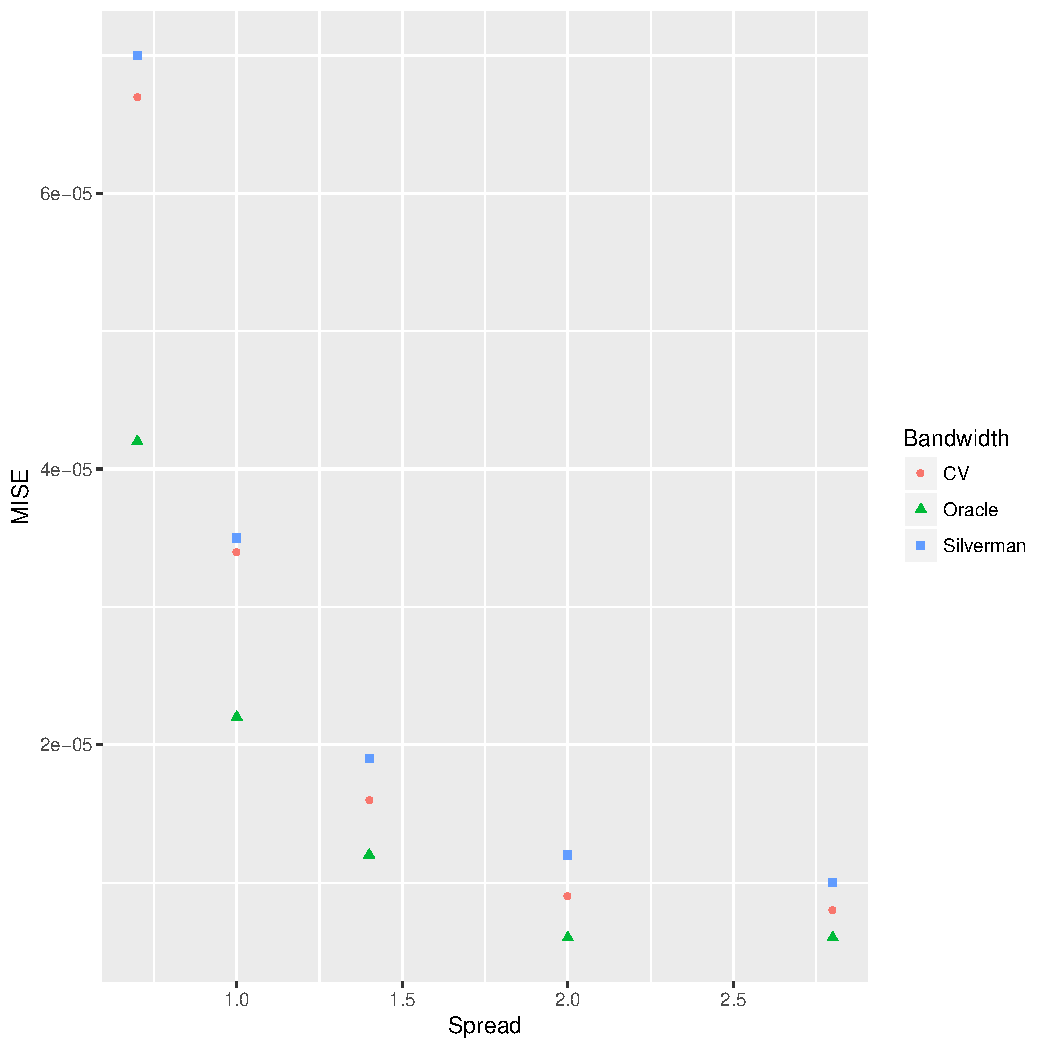
\includegraphics[width=\textwidth]{results/by_cases_spread/MISE-vs-risk-spread}
        \caption{\glsentryname{mise}}
        \label{fig:ise:unif_Spreads_1h:mise}
    \end{subfigure}
    \begin{subfigure}[t]{0.24\textwidth}
        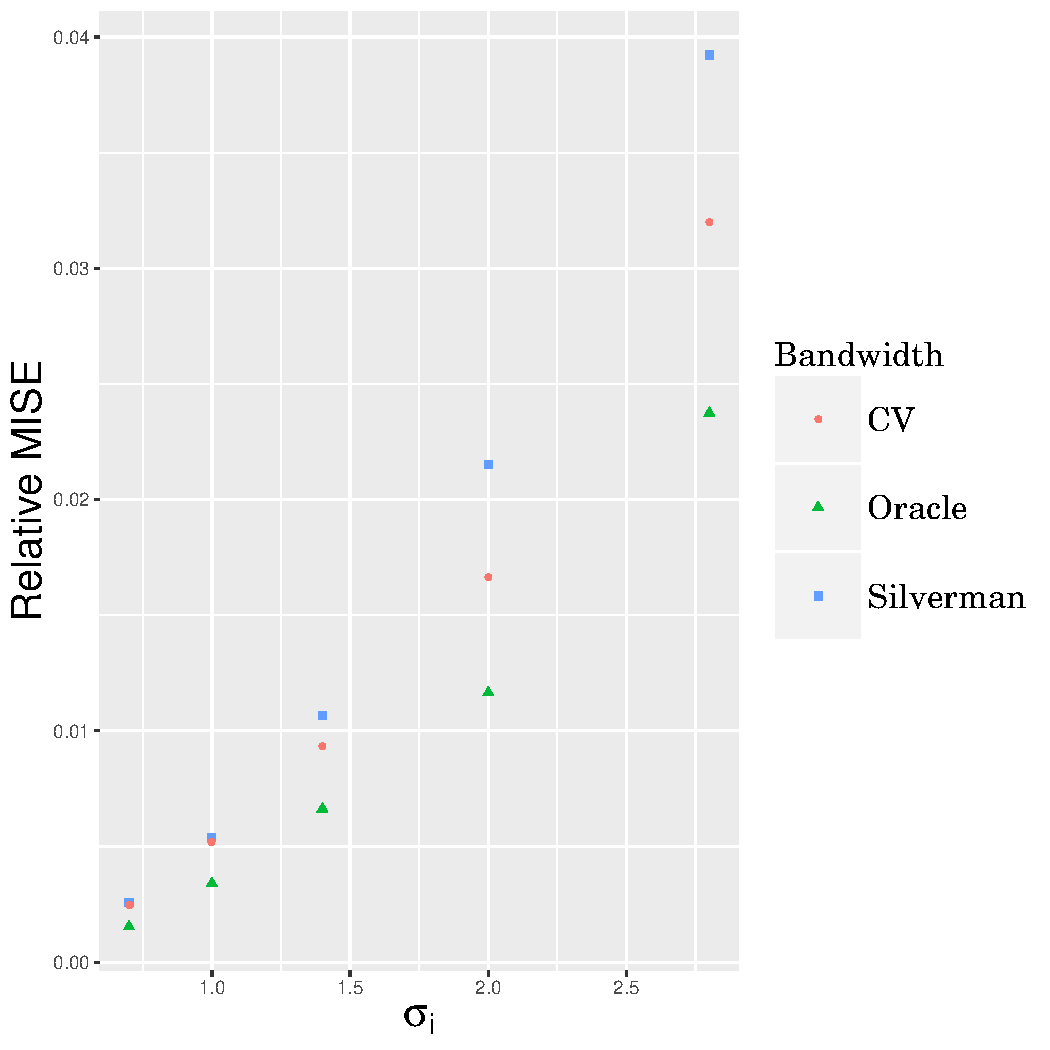
\includegraphics[width=\textwidth]{results/by_cases_spread/RMISE-vs-risk-spread}
        \caption{\glsentryname{rmise}}
        \label{fig:ise:unif_Spreads_1h:rmise}
    \end{subfigure}
    \begin{subfigure}[t]{0.24\textwidth}
        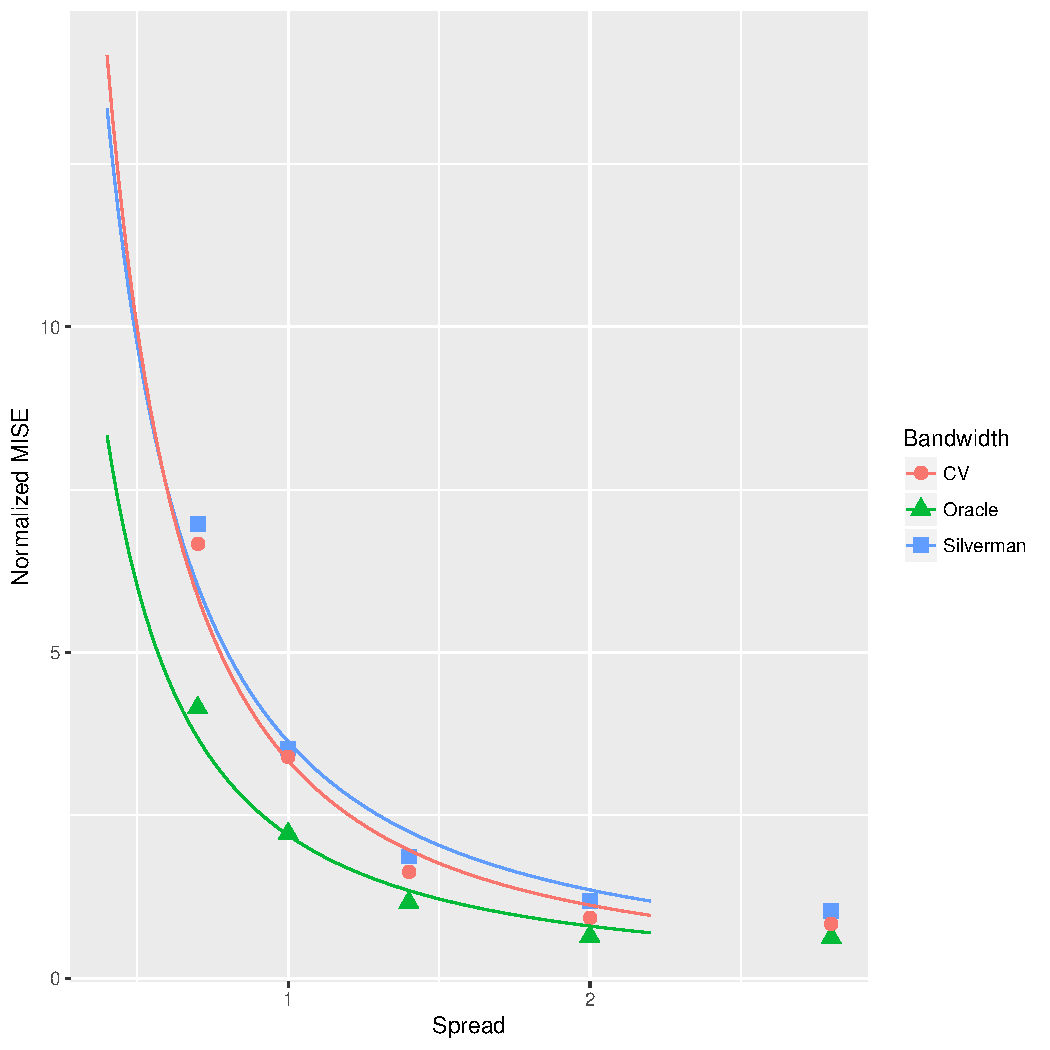
\includegraphics[width=\textwidth]{results/by_cases_spread/NMISE-vs-risk-spread}
        \caption{\glsentryname{nmise}}
        \label{fig:ise:unif_Spreads_1h:nmise}
    \end{subfigure}
    \begin{subfigure}[t]{0.24\textwidth}
        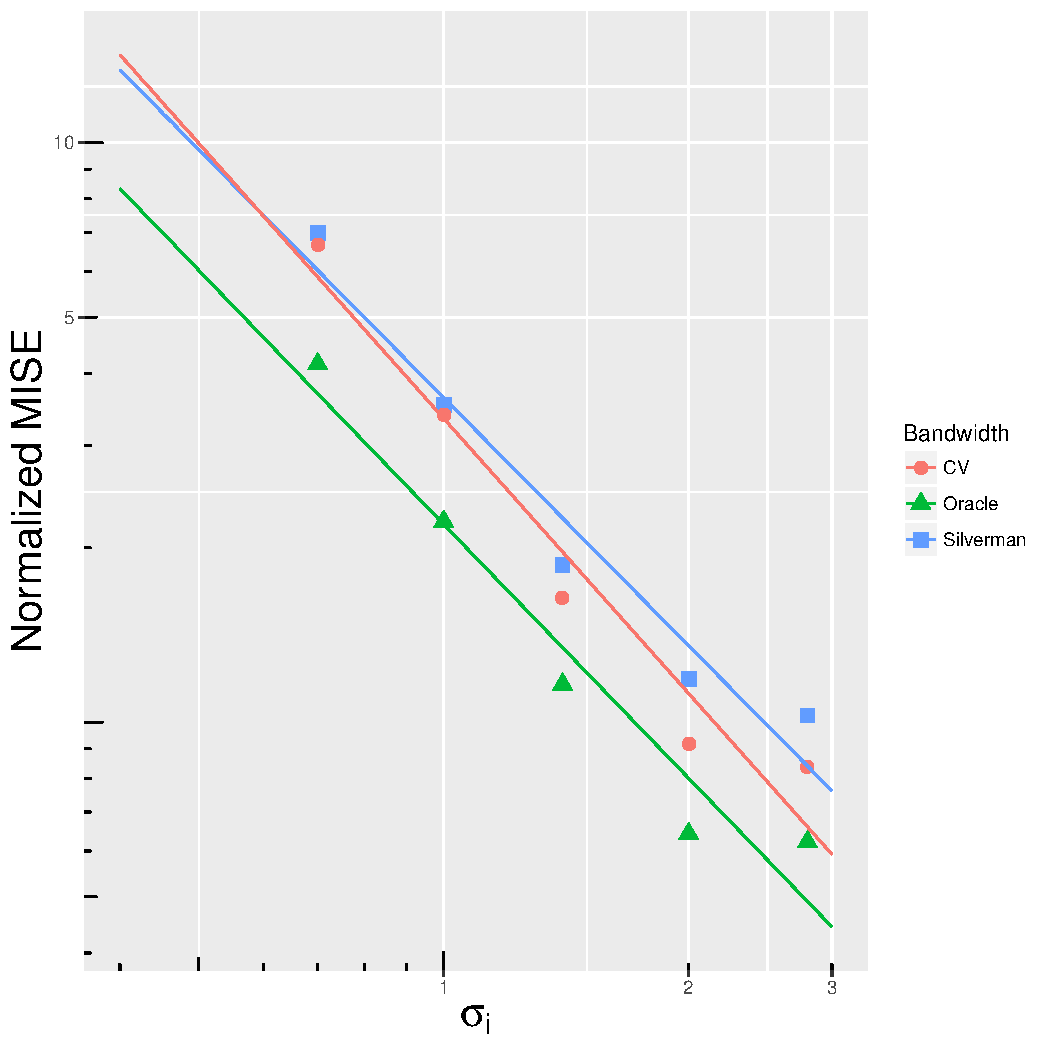
\includegraphics[width=\textwidth]{results/by_cases_spread/NMISE-vs-risk-spread-log-log}
        \caption{\glsentryname{nmise} log-log}
        \label{fig:ise:unif_Spreads_1h:nmise_log_log}
    \end{subfigure}
    \caption[\glsentryname{mise}: by risk \glsentryname{spread}]
        {The effect of \glsentryname{spread} on \glsentryname{mise} for different bandwidth selectors for a single-peak risk function with \gls{factor} 100 on a uniform population of 10,000}
    \label{fig:ise:unif_Spreads_1h}
\end{figure}

We look now at the asymptotic behavior of \gls{nmise} as $\gls{sigma_i} \to \infty$.
From \cref{fig:ise:unif_Spreads_1h:nmise_log_log} we see a polynomial relationship between \gls{nmise} and \gls{sigma_i} (\cref{eq:nmise:spread}).
\Cref{tab:results:nmise_convergence_by_cases_spread} shows the slope $\alpha_S$ that we observed for each bandwidth selection method.

\begin{equation}
    \label{eq:nmise:spread}
    \gls{nmise} = O(n^{\alpha_S})
\end{equation}
%latex.default(df.alpha, title = "nmise_convergence_table", where = "htbp",     label = "tab:results:nmise_convergence_by_cases_spread",     rowname = NULL, booktabs = TRUE, cdec = c(0, 3), caption.loc = "bottom",     caption = "NMISE convergence rate by spread for different bandwidth selectors for a single-peak risk function with expected number of incidents 100 on a uniform population of 10,000.",     caption.lot = "NMISE Convergence rate by spread for 100 cases")%
\begin{table}[htbp]
\begin{center}
\begin{tabular}{lr}
\toprule
\multicolumn{1}{c}{Selector}&\multicolumn{1}{c}{Slope}\tabularnewline
\midrule
Oracle&$-1.455$\tabularnewline
Silverman&$-1.421$\tabularnewline
CV&$-1.576$\tabularnewline
\bottomrule
\end{tabular}
\caption[NMISE Convergence rate by spread for 100 cases]{NMISE convergence rate by spread for different bandwidth selectors for a single-peak risk function with expected number of incidents 100 on a uniform population of 10,000.\label{tab:results:nmise_convergence_by_cases_spread}}\end{center}
\end{table}


We now look at the convergence rate of \gls{rmise} as the number of incidents grow.
We see from \cref{tab:results:rmise_convergence_by_cases_and_spread} that independent of bandwidth selection method,
there is no clear pattern in the convergence rates.
For each value of the \gls{spread}, there is negative polynomial convergence as incidents go to infinity.
However, we did not observe a monotonic growth rate of the exponent with the spread.

%latex.default(df, title = "rmise_convergence_table", where = "htbp",     label = "tab:results:rmise_convergence_by_cases_and_spread",     rowname = NULL, booktabs = TRUE, cdec = c(1, rep(3, 3)),     caption.loc = "bottom", caption = "RMISE convergence rates by case for different bandwidth selectors and different spreads when the population of 10,000 is uniformly distributed.",     caption.lot = "RMISE Convergence rate by case for different spreads")%
\begin{table}[htbp]
\begin{center}
\begin{tabular}{rrrr}
\toprule
\multicolumn{1}{c}{decay}&\multicolumn{1}{c}{alphaO}&\multicolumn{1}{c}{alphaS}&\multicolumn{1}{c}{alphaC}\tabularnewline
\midrule
$0.7$&$-0.301$&$-0.431$&$-0.418$\tabularnewline
$1.0$&$-0.742$&$-0.741$&$-0.775$\tabularnewline
$1.4$&$-0.666$&$-0.701$&$-0.712$\tabularnewline
$2.0$&$-0.604$&$-0.652$&$-0.670$\tabularnewline
$Inf$&$-0.327$&$-0.377$&$-0.354$\tabularnewline
\bottomrule
\end{tabular}
\caption[RMISE Convergence rate by case for different spreads]{RMISE convergence rates by case for different bandwidth selectors and different spreads when the population of 10,000 is uniformly distributed.\label{tab:results:rmise_convergence_by_cases_and_spread}}\end{center}
\end{table}



%%%%%%%%%%%%%%%%%%%%%%%%%%%%%%%%%%%%%%%%%%%%%%%%%%%%%%%%%%%%%%%%%%%%%%%%%%%%%%
%%
%% Section: Varying the sample size for fixed intensity
%%
%%%%%%%%%%%%%%%%%%%%%%%%%%%%%%%%%%%%%%%%%%%%%%%%%%%%%%%%%%%%%%%%%%%%%%%%%%%%%%
\section{Varying the population and sample size for fixed intensity}
\label{sec:results:unifNpop_1h}

%%%%%%%%%%%%%%%%%%%%%%%%%%%%%
% Parameter table
%%%%%%%%%%%%%%%%%%%%%%%%%%%%%
\begin{table}[htbp]
    \centering
    \begin{tabular}{ll}
        \toprule
        Parameter & Value \\
        \midrule
        Population size & 5,000, 10,000, 20,000, 50,000, 100,000 \\
        Population \gls{spread} & uniform \\
        Population center & uniform \\
        \Gls{factor} & 50, 100, 200, 500, 1000 \\
        Incident \gls{spread} & 1.0 \\
        Incident center & (0,0) \\
        \bottomrule
    \end{tabular}
    \caption{Parameters used for varying the sample size for fixed intensity}
    \label{tab:params:unifNpop_1h}
\end{table}

We next examine the effect of increasing the sample size, while keeping the risk intensity function fixed.
Unlike what we did in \cref{sec:results:number_of_incidents} where we fixed the size of the population and allowed the risk function to change,
here we fix the risk function and change the population size.
This is analogous to increasing the size of the population under study, for example by increasing the study area.
In order to do this, we increase the population size and the \gls{factor} proportionately.
For example, in one experiment \gls{factor} is 50 and the population is 5,000,
and in the next experiment the \gls{factor} is 100 and the population is 10,000.
For this set of experiments, the population is uniformly distributed and the risk intensity has a single peak in the center with a fixed \gls{sigma_i} of 1.0.
Mean and standard deviations of accuracy measures for the experiments of this section are found in \cref{tab:mean_error_rates:unif5k_50_1.0_1h,tab:mean_error_rates:unif10k_100_1.0_1h,tab:mean_error_rates:unif20k_200_1.0_1h,tab:mean_error_rates:unif50k_500_1.0_1h,tab:mean_error_rates:unif100k_1000_1.0_1h}.

\Cref{fig:one_sample:unifNpop_1h} shows the denser population, as represented by the blue dots, and the larger sample size, represented by the red dots.
In both cases, the population is distributed uniformly throughout the study area,
while the incident samples are concentrated around the peak in the center.

%%%%%%%%%%%%%%%%%%%%%%%%%%%%%%%%%%%%%%%%%%%%%%%%%
% Examples showing sample size
%%%%%%%%%%%%%%%%%%%%%%%%%%%%%%%%%%%%%%%%%%%%%%%%%
\begin{figure}[htbp]
    \centering
    \begin{subfigure}{0.45\textwidth}
        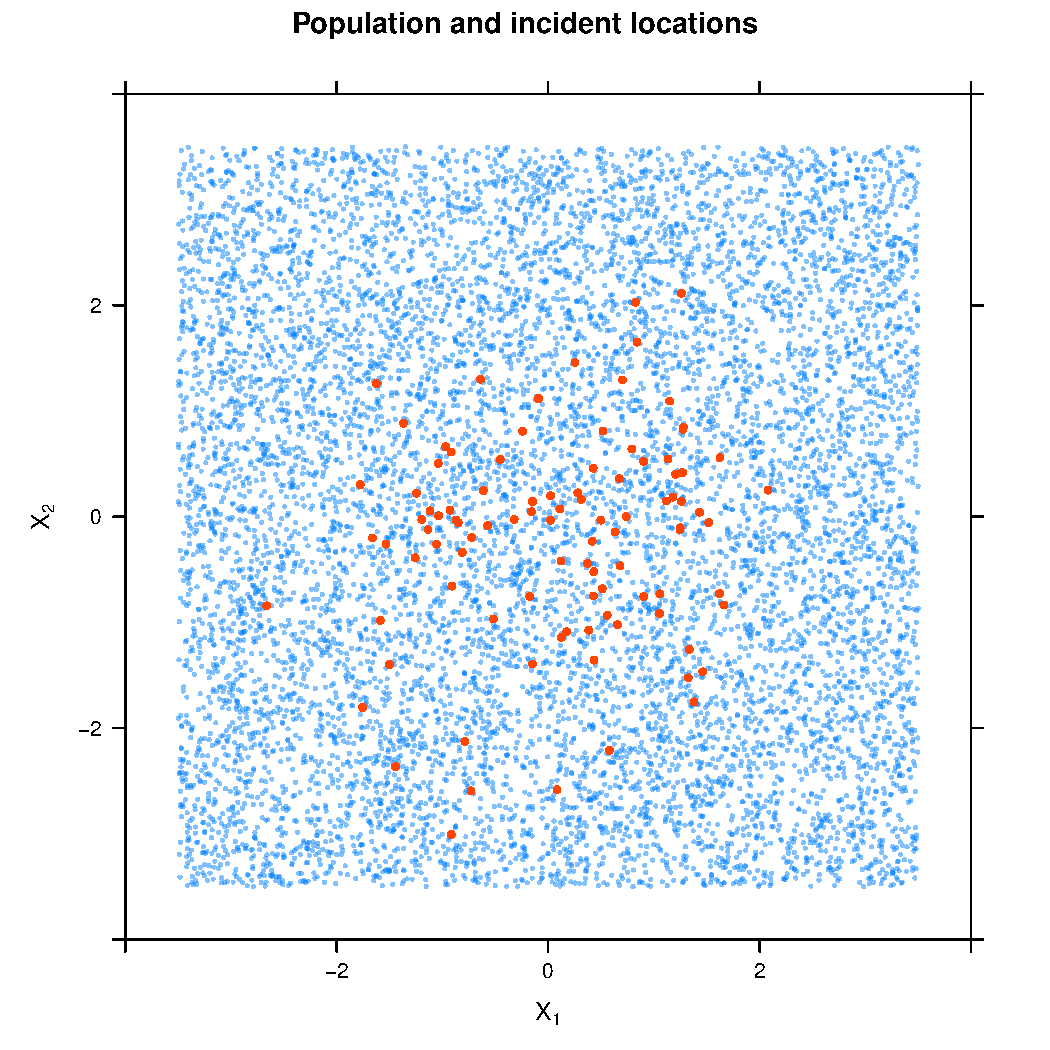
\includegraphics[width=\textwidth]{results/unif10k_100_1.0_1h/output/population_and_incidents_scatter}
        \caption{100 incidents from population of 10,000}
    \end{subfigure}
    \begin{subfigure}{0.45\textwidth}
        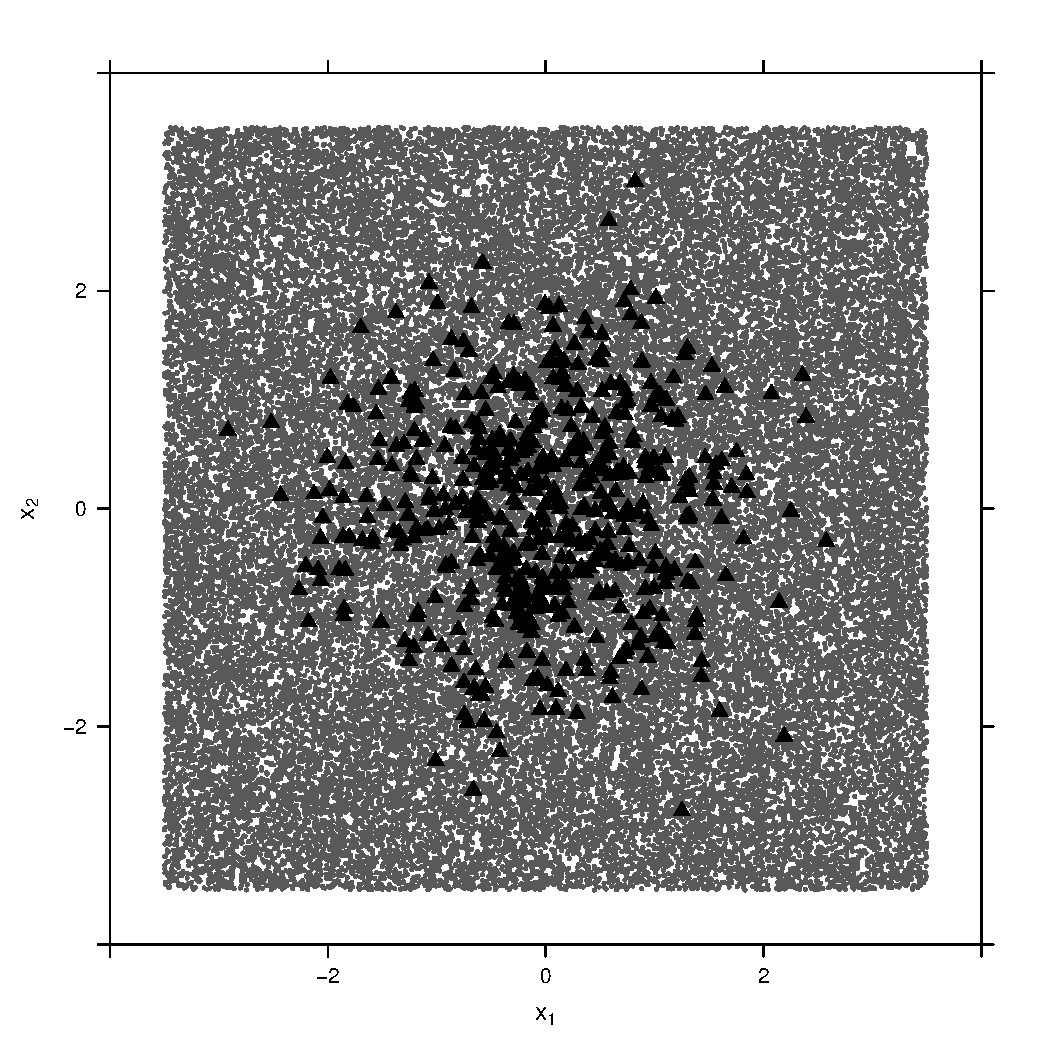
\includegraphics[width=\textwidth]{results/unif50k_500_1.0_1h/output/population_and_incidents_scatter}
        \caption{500 incidents from population of 50,000}
    \end{subfigure}
    \caption[Examples showing sample size]
        {A single realization of different sample sizes from a single-peak risk on a uniform population, obtained by varying the \gls{factor} and population size in lockstep while keeping the risk function $\lambda \xvec$ fixed}
    \label{fig:one_sample:unifNpop_1h}
\end{figure}

%%%%%%%%%%%%%%%%%%%%%%%%%%%%%%%%%%%%%%%%%%%%%%%%%
% MISE by sample + population
%%%%%%%%%%%%%%%%%%%%%%%%%%%%%%%%%%%%%%%%%%%%%%%%%
\begin{figure}[htbp]
    \centering
    \begin{subfigure}[b]{0.24\textwidth}
        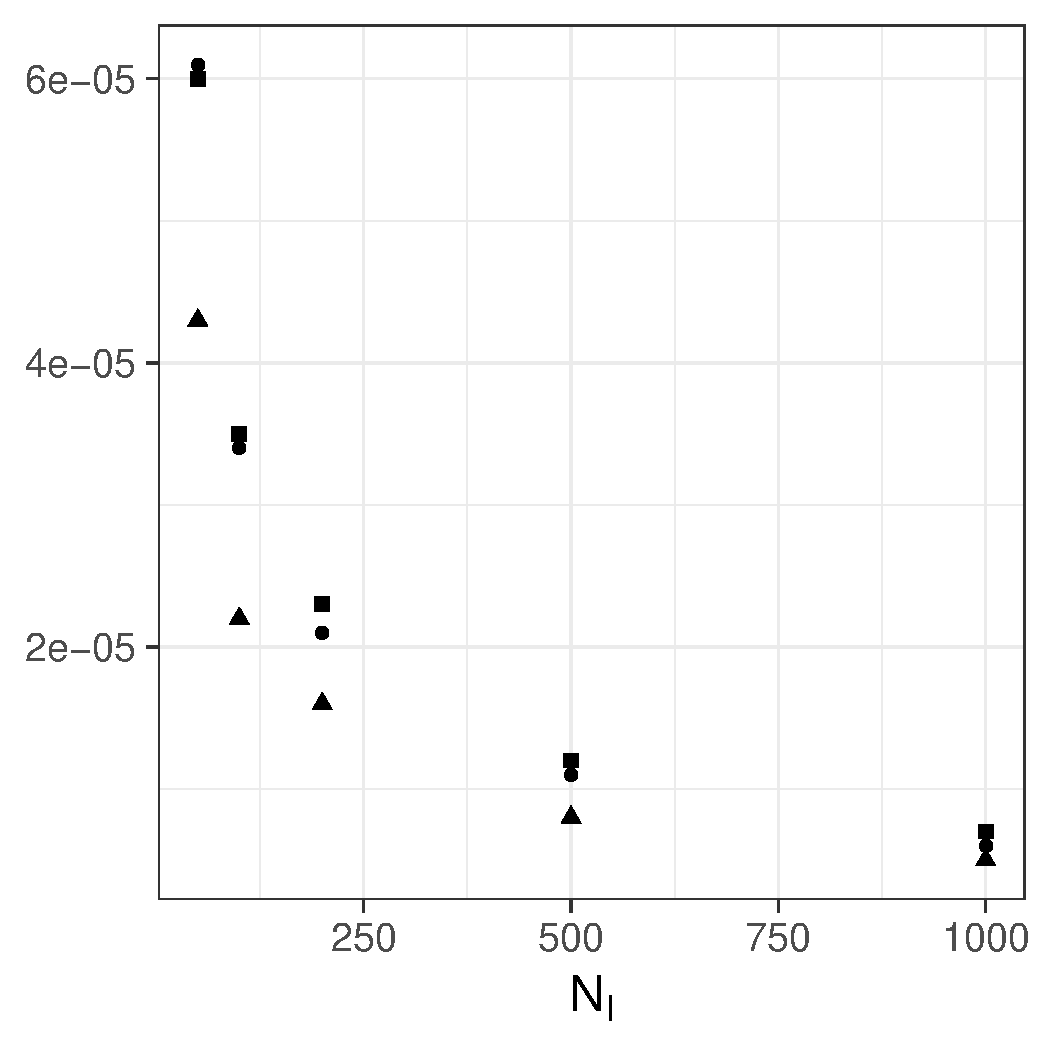
\includegraphics[width=\textwidth]{results/by_pop_size/MISE-vs-population}
        \caption{\glsentryname{mise}}
        \label{fig:ise:unifNpop_1h:mise}
    \end{subfigure}
    \begin{subfigure}[b]{0.24\textwidth}
        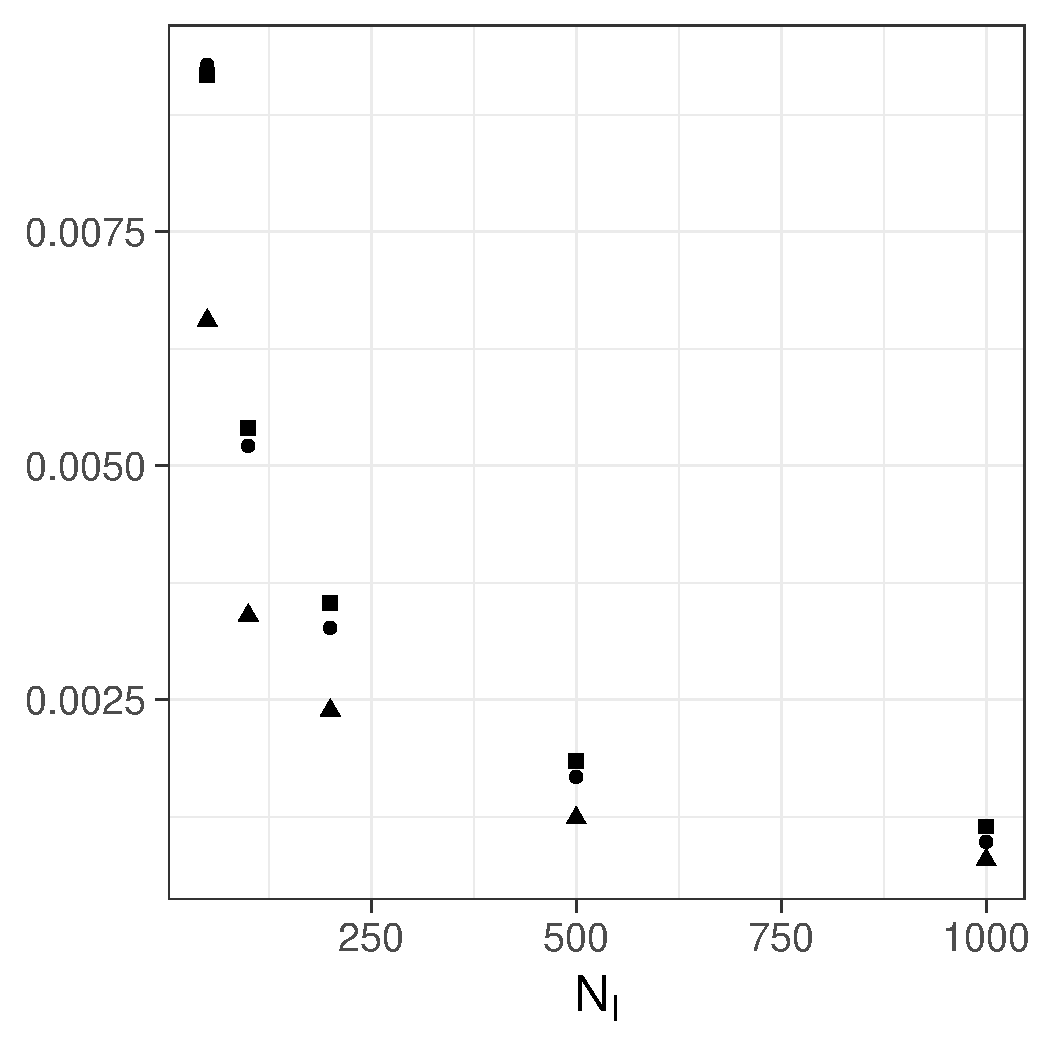
\includegraphics[width=\textwidth]{results/by_pop_size/RMISE-vs-population}
        \caption{\glsentryname{rmise}}
        \label{fig:ise:unifNpop_1h:rmise}
    \end{subfigure}
    \begin{subfigure}[b]{0.24\textwidth}
        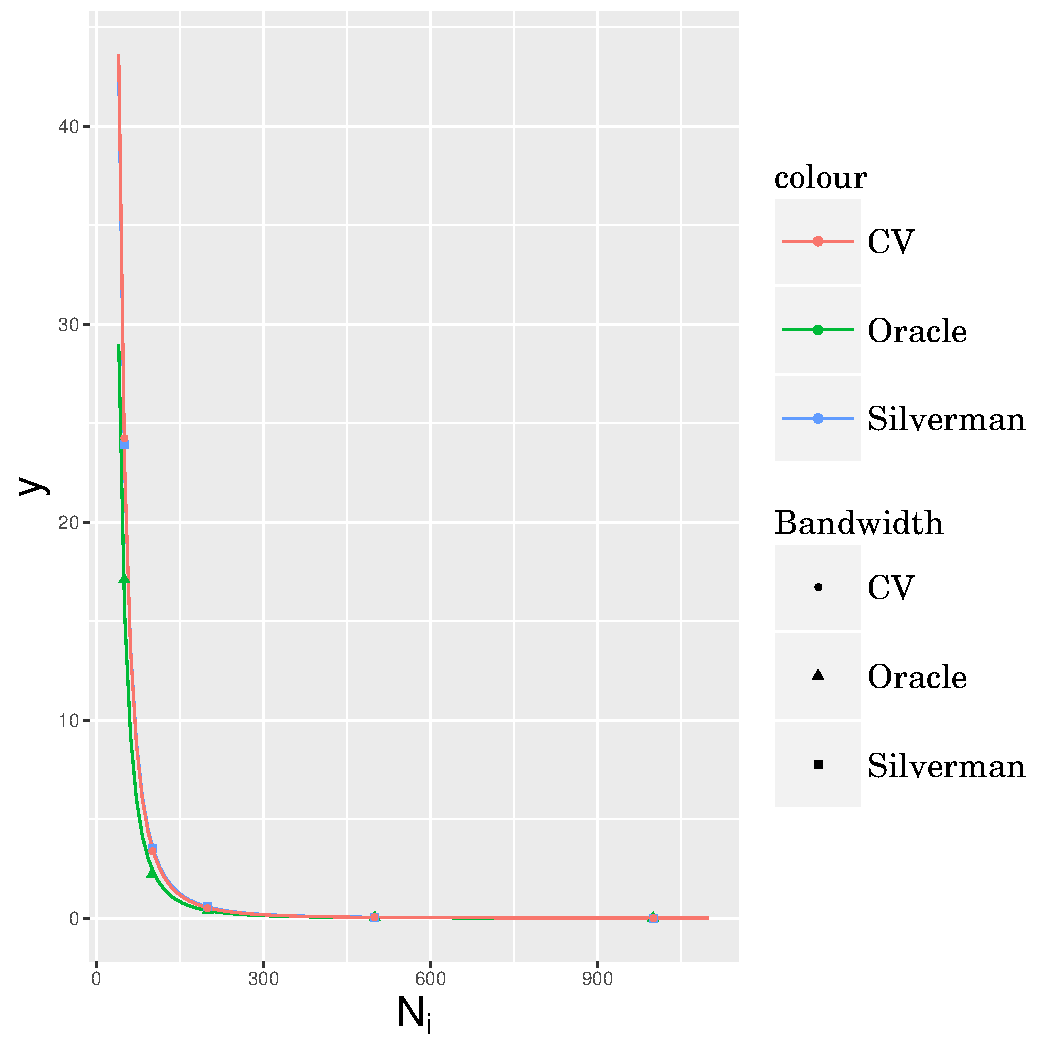
\includegraphics[width=\textwidth]{results/by_pop_size/NMISE-vs-population}
        \caption{\glsentryname{nmise}}
        \label{fig:ise:unifNpop_1h:nmise}
    \end{subfigure}
    \begin{subfigure}[b]{0.24\textwidth}
        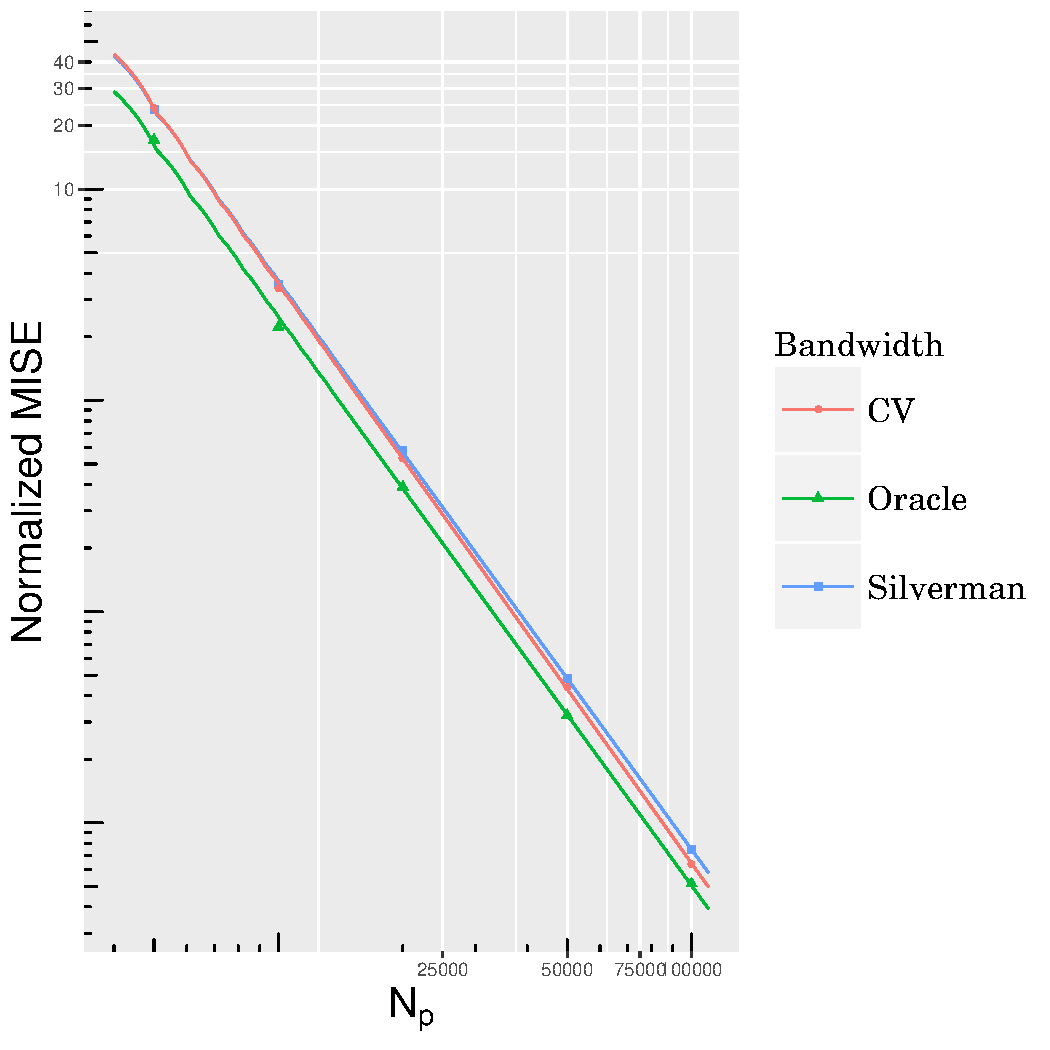
\includegraphics[width=\textwidth]{results/by_pop_size/NMISE-vs-population-log-log}
        \caption{\glsentryname{nmise} log-log}
        \label{fig:ise:unifNpop_1h:nmise_log_log}
    \end{subfigure}
    \caption[\glsentryname{mise}: by sample and population size]{\glsentryname{mise} vs. sample and population size}
    \label{fig:ise:unifNpop_1h}
\end{figure}

In \cref{fig:ise:unifNpop_1h:mise} we see that in this experiment,
\gls{mise} decreases when the sample and population sizes increase.
\Gls{rmise} also decreases in a similar manner, as shown in \cref{fig:ise:unifNpop_1h:rmise}.
When we look at \cref{fig:ise:unifNpop_1h:nmise} we see that the rate of decrease of \gls{nmise} appears to be much higher than \gls{mise}.
In \cref{tab:results:nmise_convergence_by_sample_size} we see that when we fix the risk function $\lambda \xvec$,
the \gls{nmise} converges at a much higher rate than we observed in \cref{sec:results:number_of_incidents}.
We also note that selected the bandwidth using \gls{cv} appears to result in a slightly faster rate of convergence than \gls{silverman}.

%latex.default(df.alpha, title = "nmise_convergence_table", where = "htbp",     label = "tab:results:nmise_convergence_by_sample_size", rowname = NULL,     booktabs = TRUE, cdec = c(0, 3), caption.loc = "bottom",     caption = "NMISE convergence rate by sample size for different bandwidth selectors for a fixed, single-peak risk function with expected number of incidents 100 on a uniform population.",     caption.lot = "NMISE Convergence rate by sample size")%
\begin{table}[htbp]
\begin{center}
\begin{tabular}{lr}
\toprule
\multicolumn{1}{c}{Selector}&\multicolumn{1}{c}{Slope}\tabularnewline
\midrule
Oracle&$-2.689$\tabularnewline
Silverman&$-2.688$\tabularnewline
CV&$-2.741$\tabularnewline
\bottomrule
\end{tabular}
\caption[NMISE Convergence rate by sample size]{NMISE convergence rate by sample size for different bandwidth selectors for a fixed, single-peak risk function with expected number of incidents 100 on a uniform population.\label{tab:results:nmise_convergence_by_sample_size}}\end{center}
\end{table}


Regarding the other measures of accuracy, the \gls{miae} and \gls{supremum error} both follow the same pattern as the \gls{mise}:
decreasing as $N_i \to \infty$,
\gls{cv} selected bandwidth producing slightly more accurate \gls{miae} and \glspl{supremum error} than \gls{silverman}.
However, the \gls{peak bias} of the \gls{silverman} bandwidth \glspl{dkd} is still positive, although the \gls{centroid bias} is not.
The \gls{cv} produces much more accurate estimates of \gls{peak drift} than \gls{silverman}, but consistently underestimates the \gls{peak bias} by a greater value.

%%%%%%%%%%%%%%%%%%%%%%%%%%%%%%%%%%%%%%%%%%%%%%%%%%%%%%%%%%%%%%%%%%%%%%%%%%%%%%
%%
%% Section: Varying the spread of the population density
%%
%%%%%%%%%%%%%%%%%%%%%%%%%%%%%%%%%%%%%%%%%%%%%%%%%%%%%%%%%%%%%%%%%%%%%%%%%%%%%%
\section{Varying the spread of the population density}
\label{sec:results:pSD_100_1h}

%%%%%%%%%%%%%%%%%%%%%%%%%%%%%
% Parameter table
%%%%%%%%%%%%%%%%%%%%%%%%%%%%%
\begin{table}[htbp]
    \centering
    \begin{tabular}{ll}
        \toprule
        Parameter & Value \\
        \midrule
        Population size & 10,000 \\
        Population \gls{spread} & 0.7, 1.0, 1.4, 2.0, 2.8 \\
        Population center & (0,0) \\
        \Gls{factor} & 100 \\
        Incident \gls{spread} & 1.0 \\
        Incident center & (0,0) \\
        \bottomrule
    \end{tabular}
    \caption{Parameters used for varying the \glsentryname{spread} of the population peak of 10,000}
    \label{tab:params:pSD_100_1h}
\end{table}

In this section, we compare the effect of different population distributions on the estimation of a single, fixed risk function.
In particular, we vary the \gls{spread} of the population \gls{sigma_p}.
The population size is fixed at 10,000 and centered around the origin (0,0).
We conduct five experiments, using the values 0.7, 1.0, 1.4, 2.0, and 2.8 for \gls{sigma_p}.
An important consideration is that the \gls{factor} \gls{mu} is computed under the assumption of a \textit{uniformly distributed} population.
Since our populations are not uniformly distributed, we expect that the actual number of incidents observed will differ significantly from \gls{mu}.
The results of the experiments described in this section are summarized in \cref{tab:mean_error_rates:p0.7_100_1.0_1h,tab:mean_error_rates:p1.0_100_1.0_1h,tab:mean_error_rates:p1.4_100_1.0_1h,tab:mean_error_rates:p2.0_100_1.0_1h,tab:mean_error_rates:p2.8_100_1.0_1h}.
An single realization for each of $\gls{sigma_p} = 1.0$ and $\gls{sigma_p} = 2.8$ can be seen in \cref{fig:one_sample:pSD_100_1h}.
In \subref{fig:one_sample:pSD_100_1h:1.0} we see the population more densely packed into the center.
Consequently there are more incidents,
because the population is greater in the same place that the risk of incidence is higher.

%%%%%%%%%%%%%%%%%%%%%%%%%%%%%%%%%%%%%%%%%%%%%%%%%
% Examples showing population spread
%%%%%%%%%%%%%%%%%%%%%%%%%%%%%%%%%%%%%%%%%%%%%%%%%
\begin{figure}[htbp]
    \centering
    \begin{subfigure}{0.45\textwidth}
        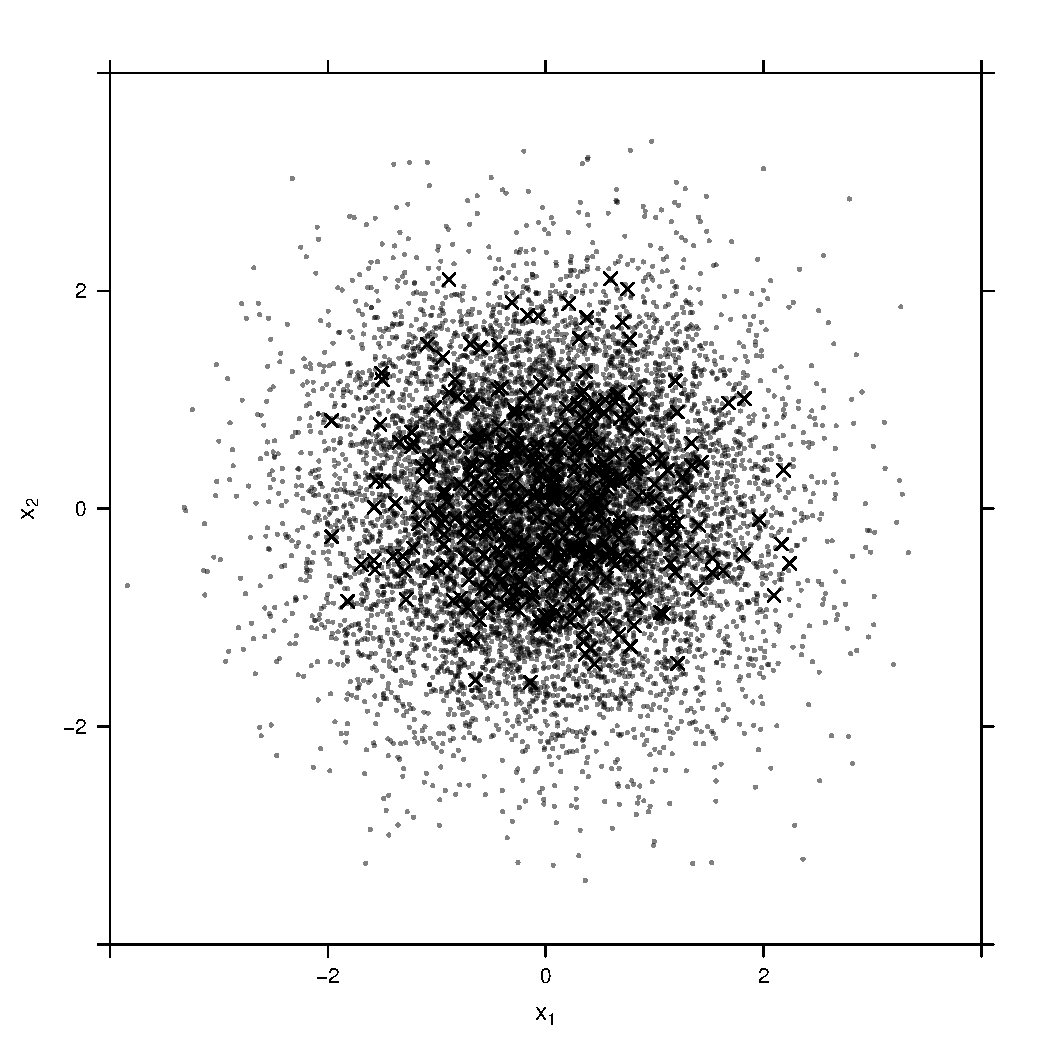
\includegraphics[width=\textwidth]{results/p1.0_100_1.0_1h/output/population_and_incidents_scatter}
        \caption{\gls{sigma_p} = 1.0}
        \label{fig:one_sample:pSD_100_1h:1.0}
    \end{subfigure}
    \begin{subfigure}{0.45\textwidth}
        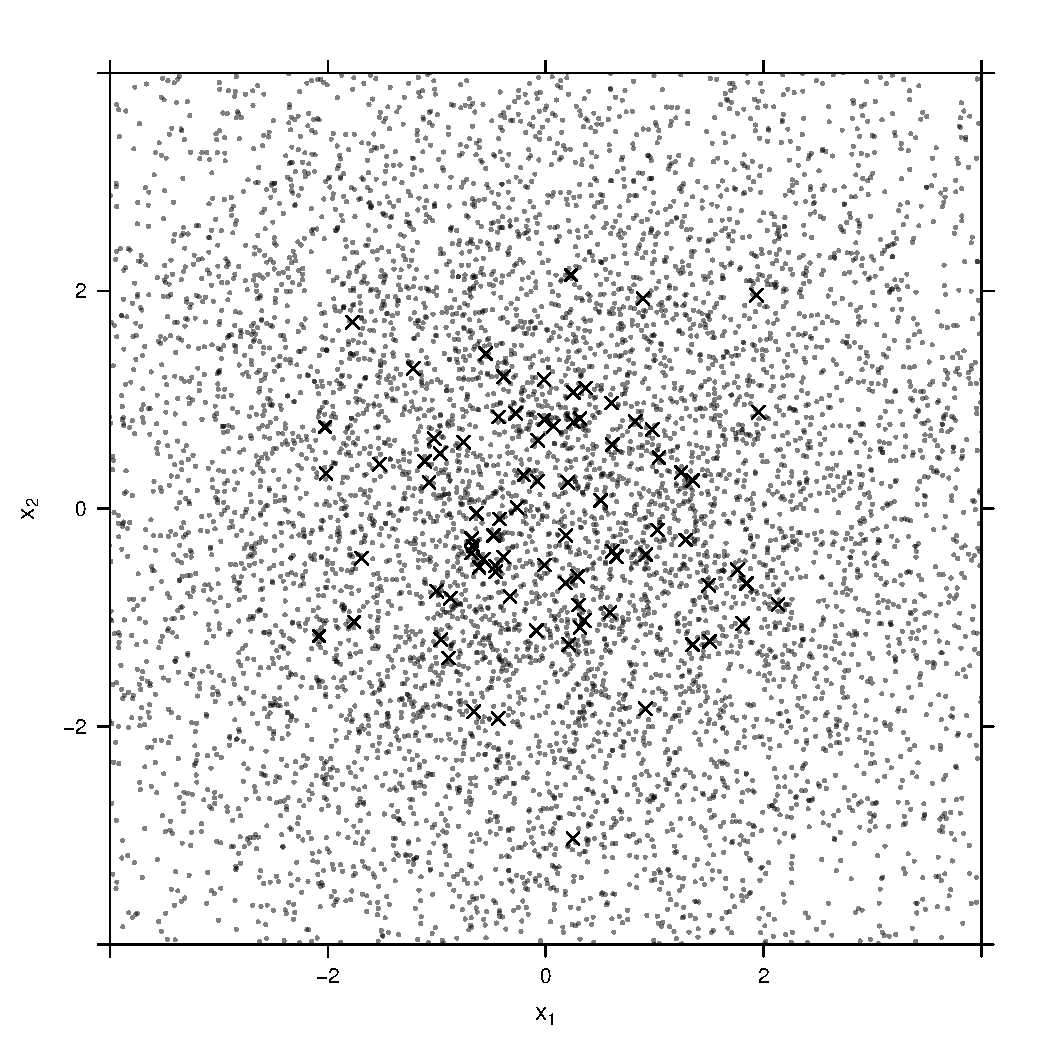
\includegraphics[width=\textwidth]{results/p2.8_100_1.0_1h/output/population_and_incidents_scatter}
        \caption{\gls{sigma_p} = 2.8}
        \label{fig:one_sample:pSD_100_1h:2.8}
    \end{subfigure}
    \caption[Examples showing population spread]
        {A single realization of different sample sizes from a single-peak risk on a single-peak population, obtained by varying the population \gls{spread} while keeping population size and the risk function $\lambda \xvec$ fixed.}
    \label{fig:one_sample:pSD_100_1h}
\end{figure}


%%%%%%%%%%%%%%%%%%%%%%%%%%%%%%%%%%%%%%%%%%%%%%%%%
% MISE by population spread
%%%%%%%%%%%%%%%%%%%%%%%%%%%%%%%%%%%%%%%%%%%%%%%%%
\begin{figure}[htbp]
    \centering
    \begin{subfigure}[t]{0.24\textwidth}
        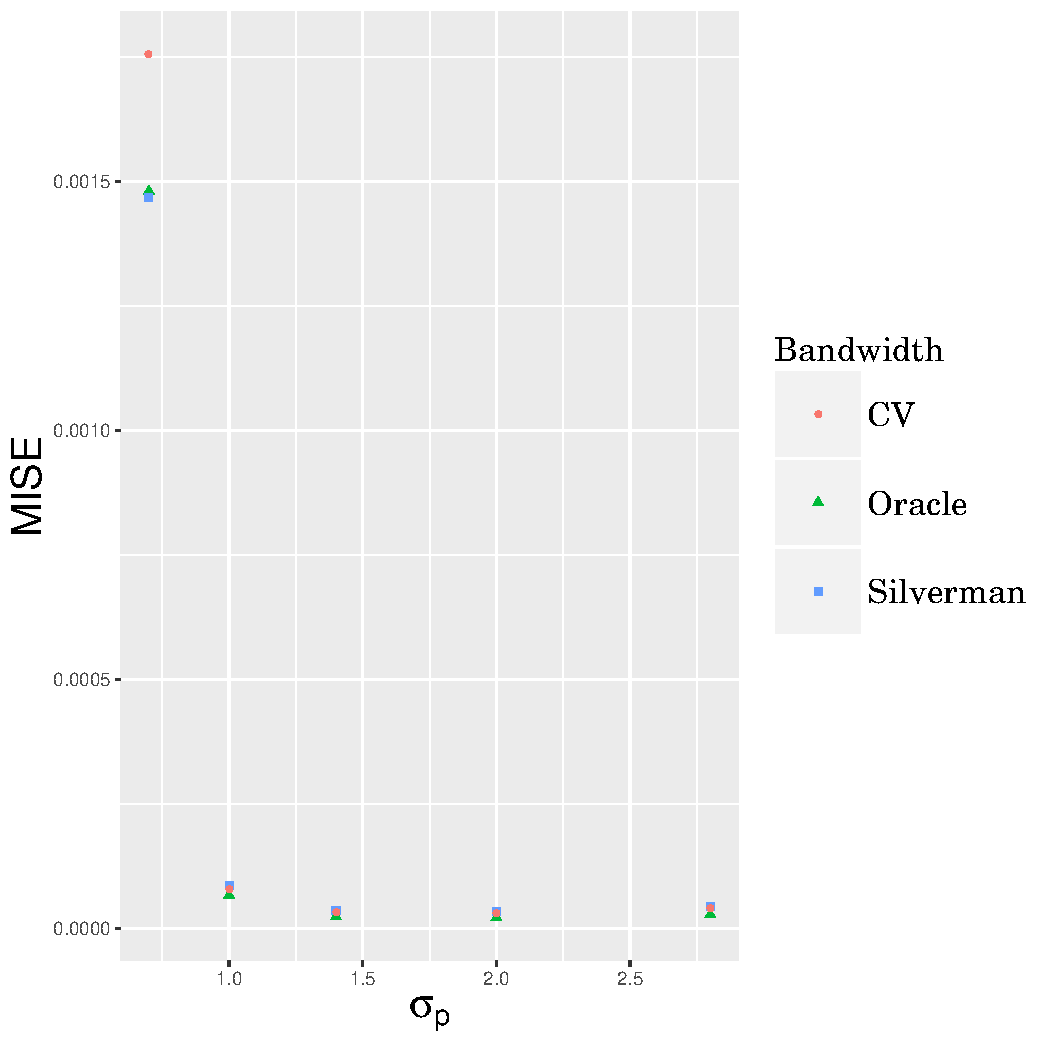
\includegraphics[width=\textwidth]{results/by_population_spread/MISE-vs-population-spread}
        \caption{\glsentryname{mise}}
        \label{fig:ise:pSD_100_1h:mise}
    \end{subfigure}
    \begin{subfigure}[t]{0.24\textwidth}
        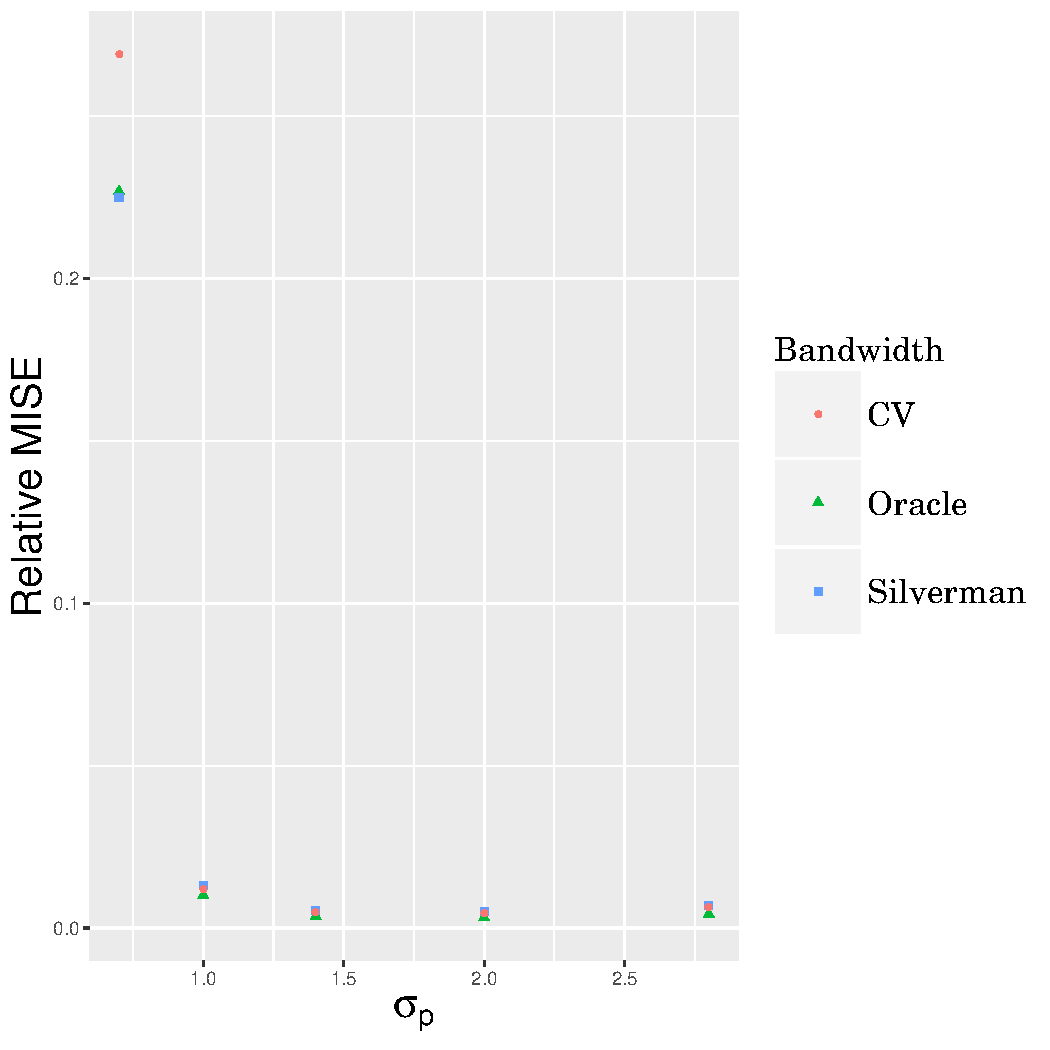
\includegraphics[width=\textwidth]{results/by_population_spread/RMISE-vs-population-spread}
        \caption{\glsentryname{rmise}}
        \label{fig:ise:pSD_100_1h:rmise}
    \end{subfigure}
    \begin{subfigure}[t]{0.24\textwidth}
        \includegraphics[width=\textwidth]{results/by_population_spread/NMISE-vs-population-spread}
        \caption{\glsentryname{nmise}}
        \label{fig:ise:pSD_100_1h:nmise}
    \end{subfigure}
    \begin{subfigure}[t]{0.24\textwidth}
        \includegraphics[width=\textwidth]{results/by_population_spread/NMISE-vs-population-spread-log-log}
        \caption{\glsentryname{nmise} log-log}
        \label{fig:ise:pSD_100_1h:nmise_log_log}
    \end{subfigure}
    \caption[\glsentryname{mise}: by population \glsentryname{spread}]{\glsentryname{mise} vs. population \glsentryname{spread}}
    \label{fig:ise:pSD_100_1h}
\end{figure}

\Cref{fig:ise:pSD_100_1h} shows how \gls{mise}, \gls{rmise} and \gls{nmise} are affected by population spread.
In \subref{fig:ise:pSD_100_1h:nmise_log_log} it does not appear that there is any linear relationship,
and there does not appear to be any convergence to zero of any of these measures as $\gls{sigma_p} \to \infty$.
In fact, it appears that as long as the population distribution does not change too rapidly,
the \gls{dkd} gives similar performance for any population \gls{spread}.

Regarding the other accuracy measures, we see that \gls{miae} and \gls{supremum error} are similar,
in that for $\gls{sigma_p} = 0.7$ the values are very high,
but they are generally low for other values of \gls{sigma_p}.
Because the risk function $\gls{lambda} \xvec$ is identical across experiments,
the relative, normal and absolute measures all have similar patterns
as seen in \cref{fig:other_measures:pSD_100_1h}.

%%%%%%%%%%%%%%%%%%%%%%%%%%%%%%%%%%%%%%%%%%%%%%%%%
% Other accuracy measures by population spread
%%%%%%%%%%%%%%%%%%%%%%%%%%%%%%%%%%%%%%%%%%%%%%%%%
\begin{figure}[htbp]
    \centering
    \begin{subfigure}[t]{0.24\textwidth}
        \includegraphics[width=\textwidth]{results/by_population_spread/MIAE-vs-population-spread}
        \caption{\glsentryname{miae}}
        \label{fig:other_measures:pSD_100_1h:miae}
    \end{subfigure}
    \begin{subfigure}[t]{0.24\textwidth}
        \includegraphics[width=\textwidth]{results/by_population_spread/maxerr-vs-population-spread}
        \caption{\Gls{supremum error}}
        \label{fig:other_measures:pSD_100_1h:maxerr}
    \end{subfigure}
    \caption{\glsentryname{miae} and \Gls{supremum error} by population \glsentryname{spread}}
    \label{fig:other_measures:pSD_100_1h}
\end{figure}

%%%%%%%%%%%%%%%%%%%%%%%%%%%%%%%%%%%%%%%%%%%%%%%%%%%%%%%%%%%%%%%%%%%%%%%%%%%%%%
%%
%% Section: Distance between two peaks
%%
%%%%%%%%%%%%%%%%%%%%%%%%%%%%%%%%%%%%%%%%%%%%%%%%%%%%%%%%%%%%%%%%%%%%%%%%%%%%%%
\section{Distance between two peaks}
\label{sec:results:p1.4_100_G}

%%%%%%%%%%%%%%%%%%%%%%%%%%%%%
% Parameter table
%%%%%%%%%%%%%%%%%%%%%%%%%%%%%
\begin{table}[htbp]
    \centering
    \begin{tabular}{ll}
        \toprule
        Parameter & Value \\
        \midrule
        Population size & 10,000 \\
        Population \gls{spread} & uniform \\
        Population center & uniform \\
        \Gls{factor} & 40, 60 \\
        Incident \gls{spread} & 1.0 \\
        Incident center & \{(0.5,0), (-0.5,0)\},  \{(1,0), (-1,0)\}, \{(1.5,0), (-1.5,0)\}, \{(2,0), (-2,0)\}\\
        \bottomrule
    \end{tabular}
    \caption{Parameters used for varying the two peaks of the risk function with \glspl{factor} 40 and 60 on a uniform population of 10,000}
    \label{tab:params:p1.4_100_G}
\end{table}

In this section, we look at incident risk functions that have two peaks.
The major peak has a \gls{factor} of 60, while the second, minor peak has a \gls{factor} of 40.
We do this to see how the minor peak affects the accuracy of the measuring the \gls{dkd} in general and the \gls{peak bias} and \gls{peak drift} in particular.
The results of the experiments described in this section are summarized in \cref{tab:mean_error_rates:unif_100_1_2h_1,tab:mean_error_rates:unif_100_1_2h_2,tab:mean_error_rates:unif_100_1_2h_3,tab:mean_error_rates:unif_100_1_2h_4}.

%%%%%%%%%%%%%%%%%%%%%%%%%%%%%%%%%%%%%%%%%%%%%%%%%
% Examples showing distance between two peaks
%%%%%%%%%%%%%%%%%%%%%%%%%%%%%%%%%%%%%%%%%%%%%%%%%
\begin{figure}[htbp]
    \centering
    \begin{subfigure}{0.45\textwidth}
        \includegraphics[width=\textwidth]{results/unif_100_1_2h_2/output/population_and_incidents_scatter}
        \subcaption{Centers at $\{(1,0), (-1,0)\}$ (distance 2)}
        \label{fig:one_sample:p1.4_100_G:2}
    \end{subfigure}
    \begin{subfigure}{0.45\textwidth}
        \includegraphics[width=\textwidth]{results/unif_100_1_2h_4/output/population_and_incidents_scatter}
        \subcaption{Centers at $\{(2,0), (-2,0)\}$ (distance 4)}
        \label{fig:one_sample:p1.4_100_G:4}
    \end{subfigure}
    \caption[Examples showing distance between two peaks]
        {A single realization of different sample sizes from a double-peak risk on a uniform population, obtained by varying the distance between two peaks in the incident risk function.}
    \label{fig:one_sample:p1.4_100_G}
\end{figure}


%%%%%%%%%%%%%%%%%%%%%%%%%%%%%%%%%%%%%%%%%%%%%%%%%
% MISE by peak distance
%%%%%%%%%%%%%%%%%%%%%%%%%%%%%%%%%%%%%%%%%%%%%%%%%
\begin{figure}[htbp]
    \centering
    \begin{subfigure}[b]{0.24\textwidth}
        \includegraphics[width=\textwidth]{results/by_two_peaks/MISE-vs-risk-peak-gap}
        \caption{\glsentryname{mise}}
    \end{subfigure}
    \begin{subfigure}[b]{0.24\textwidth}
        \includegraphics[width=\textwidth]{results/by_two_peaks/RMISE-vs-risk-peak-gap}
        \caption{\glsentryname{rmise}}
    \end{subfigure}
    \begin{subfigure}[b]{0.24\textwidth}
        \includegraphics[width=\textwidth]{results/by_two_peaks/NMISE-vs-risk-peak-gap}
        \caption{\glsentryname{nmise}}
    \end{subfigure}
    \caption{\gls{mise} by distance between two risk peaks}
    \label{fig:ise:p1.4_100_G}
\end{figure}

%%%%%%%%%%%%%%%%%%%%%%%%%%%%%%%%%%%%%%%%%%%%%%%%%
% Other measures by peak distance
%%%%%%%%%%%%%%%%%%%%%%%%%%%%%%%%%%%%%%%%%%%%%%%%%
\begin{figure}[htbp]
    \centering
    \begin{subfigure}[b]{0.24\textwidth}
        \includegraphics[width=\textwidth]{results/by_two_peaks/peak-bias-vs-risk-peak-gap}
        \caption{\glsentryname{peak bias}}
        \label{fig:other_measures:p1.4_100_G:peak_bias}
    \end{subfigure}
    \begin{subfigure}[b]{0.24\textwidth}
        \includegraphics[width=\textwidth]{results/by_two_peaks/peak-drift-vs-risk-peak-gap}
        \caption{\glsentryname{peak drift}}
        \label{fig:other_measures:p1.4_100_G:peak_drift}
    \end{subfigure}
    \begin{subfigure}[b]{0.24\textwidth}
        \includegraphics[width=\textwidth]{results/by_two_peaks/centroid-bias-vs-risk-peak-gap}
        \caption{\glsentryname{centroid bias}}
        \label{fig:other_measures:p1.4_100_G:centroid_bias}
    \end{subfigure}
    \begin{subfigure}[b]{0.24\textwidth}
        \includegraphics[width=\textwidth]{results/by_two_peaks/centroid-drift-vs-risk-peak-gap}
        \caption{\glsentryname{centroid drift}}
        \label{fig:other_measures:p1.4_100_G:centroid_drift}
    \end{subfigure}
    \caption{Other accuracy measures by distance between two risk peaks}
    \label{fig:other_measures:p1.4_100_G}
\end{figure}

We observe that \gls{mise}, \gls{rmise} and \gls{nmise} all increase when the distance between two peaks increases (\cref{fig:ise:p1.4_100_G}).
The \gls{peak drift} and \gls{centroid drift} also increase when the distance between the two peaks increases (\cref{fig:other_measures:p1.4_100_G:peak_drift,fig:other_measures:p1.4_100_G:centroid_drift}).
However, we also observe that \gls{peak bias} and \gls{centroid bias} decrease as the distance between the two peaks increases (\cref{fig:other_measures:p1.4_100_G:peak_bias,fig:other_measures:p1.4_100_G:centroid_bias}).


%%%%%%%%%%%%%%%%%%%%%%%%%%%%%%%%%%%%%%%%%%%%%%%%%%%%%%%%%%%%%%%%%%%%%%%%%%%%%%
%%
%% Section: Distance between the population and risk function peaks
%%
%%%%%%%%%%%%%%%%%%%%%%%%%%%%%%%%%%%%%%%%%%%%%%%%%%%%%%%%%%%%%%%%%%%%%%%%%%%%%%
\section{Distance between the population and risk function peaks}
\label{sec:ise:p1.4_Gap_risk}

%%%%%%%%%%%%%%%%%%%%%%%%%%%%%
% Parameter table
%%%%%%%%%%%%%%%%%%%%%%%%%%%%%
\begin{table}[htbp]
    \centering
    \begin{tabular}{ll}
        \toprule
        Parameter & Value \\
        \midrule
        Population size & 10,000 \\
        Population \gls{spread} & 1.4 \\
        Population center & (-0.5,0), (-1,0), (-1.5,0), (-2,0) \\
        \Gls{factor} & 40, 60 \\
        Incident \gls{spread} & 1.0 \\
        Incident center & (0.5,0), (1,0), (1.5,0), (2,0) \\
        \bottomrule
    \end{tabular}
    \caption{Parameters used for varying the peak of the single-peak risk function with \glspl{factor} 100 and the peak of the single-peak population of 10,000}
    \label{tab:params:p1.4_100_Gap_risk}
\end{table}

In this section, we look at incident risk function that have their peak at a different location from the peak in the population distribution.
We expect that as this distance grows, the relatively small population at the peak of the incident risk will make it difficult to obtain any information through observing incidents and estimating with the \gls{dkd}.
The results of the experiments described in this section are summarized in \cref{tab:mean_error_rates:p1.4_100_1_1h_1s,tab:mean_error_rates:p1.4_100_1_1h_2s,tab:mean_error_rates:p1.4_100_1_1h_3s,tab:mean_error_rates:p1.4_100_1_1h_4s}.

%%%%%%%%%%%%%%%%%%%%%%%%%%%%%%%%%%%%%%%%%%%%%%%%%
% Examples showing distance between population
% and incident peaks
%%%%%%%%%%%%%%%%%%%%%%%%%%%%%%%%%%%%%%%%%%%%%%%%%
\begin{figure}[htbp]
    \centering
    \begin{subfigure}{0.45\textwidth}
        \includegraphics[width=\textwidth]{results/p1.4_100_1_1h_2s/output/population_and_incidents_scatter}
        \subcaption{Centers at $\{(-1,0), (1,0)\}$ (distance 2)}
        \label{fig:one_sample:p1.4_100_Gap_risk:2}
    \end{subfigure}
    \begin{subfigure}{0.45\textwidth}
        \includegraphics[width=\textwidth]{results/p1.4_100_1_1h_4s/output/population_and_incidents_scatter}
        \subcaption{Centers at $\{(-2,0), (2,0)\}$ (distance 4)}
        \label{fig:one_sample:p1.4_100_Gap_risk:4}
    \end{subfigure}
    \caption[Examples showing distance between population and incident peaks]
        {A single realization of different sample sizes from a single-peak risk on a single-peak population, obtained by varying the distance between two peaks.}
    \label{fig:one_sample:p1.4_100_Gap_risk}
\end{figure}

%%%%%%%%%%%%%%%%%%%%%%%%%%%%%%%%%%%%%%%%%%%%%%%%%
% MISE by distance between population
% and incident peaks
%%%%%%%%%%%%%%%%%%%%%%%%%%%%%%%%%%%%%%%%%%%%%%%%%
\begin{figure}[htbp]
    \centering
    \begin{subfigure}[b]{0.24\textwidth}
        \includegraphics[width=\textwidth]{results/by_pop_risk_distance/MISE-vs-population-risk-gap}
        \caption{\glsentryname{mise}}
        \label{fig:ise:p1.4_100_Gap_risk:mise}
    \end{subfigure}
    \begin{subfigure}[b]{0.24\textwidth}
        \includegraphics[width=\textwidth]{results/by_pop_risk_distance/RMISE-vs-population-risk-gap}
        \caption{\glsentryname{rmise}}
        \label{fig:ise:p1.4_100_Gap_risk:rmise}
    \end{subfigure}
    \begin{subfigure}[b]{0.24\textwidth}
        \includegraphics[width=\textwidth]{results/by_pop_risk_distance/NMISE-vs-population-risk-gap}
        \caption{\glsentryname{nmise}}
        \label{fig:ise:p1.4_100_Gap_risk:nmise}
    \end{subfigure}

    \begin{subfigure}[b]{0.24\textwidth}
        \includegraphics[width=\textwidth]{results/by_pop_risk_distance/RMISE-vs-population-risk-gap-log-log}
        \caption{Log-log of \glsentryname{rmise}}
        \label{fig:ise:p1.4_100_Gap_risk:rmise_log_log}
    \end{subfigure}
    \begin{subfigure}[b]{0.24\textwidth}
        \includegraphics[width=\textwidth]{results/by_pop_risk_distance/NMISE-vs-population-risk-gap-log-log}
        \caption{Log-log of \glsentryname{nmise}}
        \label{fig:ise:p1.4_100_Gap_risk:nmise_log_log}
    \end{subfigure}    
    \caption{\gls{mise} by distance between two risk peaks}
    \label{fig:ise:p1.4_100_Gap_risk}
\end{figure}

%latex.default(df.alpha, title = "nmise_convergence_table", where = "htbp",     label = "tab:results:nmise_convergence_by_pop_incident_gap",     rowname = NULL, booktabs = TRUE, cdec = c(0, 3), caption.loc = "bottom",     caption = "NMISE convergence rate by incident-population peak distance for different bandwidth selectors for a single-peak risk function with spread of 1.0 on a single-peak population of 10,000.",     caption.lot = "NMISE Convergence rate by incident-population peak distance")%
\begin{table}[htbp]
\begin{center}
\begin{tabular}{lr}
\toprule
\multicolumn{1}{c}{Selector}&\multicolumn{1}{c}{Gap}\tabularnewline
\midrule
Oracle&$1.110$\tabularnewline
Silverman&$1.055$\tabularnewline
CV&$1.181$\tabularnewline
\bottomrule
\end{tabular}
\caption[NMISE Convergence rate by incident-population peak distance]{NMISE convergence rate by incident-population peak distance for different bandwidth selectors for a single-peak risk function with spread of 1.0 on a single-peak population of 10,000.\label{tab:results:nmise_convergence_by_pop_incident_gap}}\end{center}
\end{table}


\Cref{fig:ise:p1.4_100_Gap_risk} shows the different measures of \gls{mise} accuracy.
We can see from \cref{fig:ise:p1.4_100_Gap_risk:rmise_log_log,fig:ise:p1.4_100_Gap_risk:nmise_log_log} that there is a linear relationship in the log-log graph,
indicating polynomial increase with positive coefficient of \gls{mise} when the distance between the incident and population peaks increases.
We see in \cref{tab:results:nmise_convergence_by_pop_incident_gap} that the exponent is just over 1,
indicating just worse than linear.


\graphicspath{{./}}


\chapter{Discussion}
\label{ch:discussion}
% !TEX root = thesis.tex

%%
%%
%% Discussion chapter
%%
%%

%The contribution of this thesis is an empirical statistical analysis of the accuracy of the \gls{dkd}
%as a tool for estimating the incidence risk of chronic diseases.
In this research we studied how different factors of the population and incidence distributions
affect the \textit{accuracy} of the \gls{dkd}.
We examined the effect of several factors on the \gls{dkd} accuracy,
and we measured the accuracy of the \gls{dkd} using \gls{mise},
\gls{miae}, \gls{supremum error}, as well as \gls{peak bias},
\gls{peak drift} and \gls{centroid bias} and \gls{centroid drift},
as described in \Cref{sec:method:accuracy}.
We ran several scenarios to examine how variations in these factors which affect the incidence risk function,
the population distribution, and the sample size affect the accuracy of \gls{dkd} for estimation.
We compared two bandwidth selection techniques, \gls{silverman}'s rule of thumb,
and least-squares \glsentrylong{cv},
both optimized to minimize \gls{mise}.
We also compared these two techniques to an \gls{oracle},
which is an approximation of the theoretical optimal bandwidth,
keeping in mind that the oracle is only computable for simulations because we know the true function we wish to estimate.

Each scenario consisted of a set of experiments,
with each experiment consisting of 1,000 monte carlo simulations.
Each simulation was a random realization of the experimental setup.
In this way,
we obtained empirical estimates of each of the above accuracy measures for the \gls{dkd}
for each bandwidth selection technique.
However,
we found that the computations of each experiment required a lot of time,
and so we tried several methods to reduce this time.
We attempted to speed up the cross-validation bandwidth selection by using gradient descent.
We found the gradient descent algorithm often resulted in severe oversmoothing,
as the cross-validation error would decrease slowly as the bandwidth increased.
This required a lot of manual tuning of the learning rate parameter,
and so required re-running the experiment several times.
We added \textit{momentum} to our gradient descent implementation but it did not help in every case,
and so we changed our strategy to use parallelization as described in \Cref{sec:method:experiment_structure}.

We observed that the estimation errors observed using the \gls{silverman} Rule of Thumb bandwidth selection method
were nearly as good as \gls{cv} in every case.
Since computing the \gls{silverman} bandwidth is much simpler than \gls{cv},
it would seem that using \gls{silverman} is warranted as a preliminary step such as for exploratory analysis.
However,
we note that in \Cref{tab:mean_error_rates:p0.7_100_1.0_1h} the accuracy measure \gls{mise} using the \gls{silverman} rule of thumb is even better than was obtained using the \gls{oracle}.
We tried to run with an additional experiment using 499 monte carlo simulations instead of 49 to compute the oracle bandwidth,
and found that in this case the \gls{silverman} rule did not outperform the \gls{oracle}.

We found that estimating the peak of the true function using the global maximum value can be improved upon.
Our method of using the 5\% centroid gave better results for both the magnitude and location of the peak most of the time.

Our results for those experiments which consist of different \gls{risk} functions on
\textbf{uniform populations},
that is,
for those for which the \gls{dkd} reduces to a kernel intensity estimate
have lower estimation errors than those which estimate
\gls{risk} functions on population distributions with a single peak.
This indicates that the population distribution has a noticeable negative effect on the accuracy of the \gls{dkd}.

%%%%%%%%%%%%%%%%%%%%%%%%%%%%%%%%%%%%%%%%%%%%%%%%%%%%%%%%%%%%%%%%%%%%%%%%%%%%%%
%%
%% Section: Limitations
%%
%%%%%%%%%%%%%%%%%%%%%%%%%%%%%%%%%%%%%%%%%%%%%%%%%%%%%%%%%%%%%%%%%%%%%%%%%%%%%%
\section{Limitations}
\label{sec:discussion:limitations}

This study uses simulated data,
sampled from a known ``true'' incidence rate function in order to measure the accuracy of the \gls{dkd} estimator.
This is quite different from what is done in a typical epidemiological study,
where population and incident locations are acquired from such sources as government and medical records,
while the rate is estimated using statistical inference.
This allows us,
in our study,
to precisely compute the measures of accuracy as deviations from the true values,
which cannot be done in scientific studies where the true incidence rate function is not known beforehand.

However,
our population and incidence rate functions,
which allow us to compute the population and incidents at points in the plane,
do not completely represent any actual population or incidents.
Nor is our study area representative of any actual populated area.
Rather,
these simplifications allow us to examine the effects of different attributes of the above functions,
by allowing us to control these factors in different experimental setups.
However,
this means that our results describe the sensitivity of the \gls{dkd} to these factors in general,
but do not provide any guarantees about the accuracy of the \gls{dkd} in any specific study where it has been used.

Another limitation of this study is that we compared only two bandwidth selection techniques.
There are several techniques available that we did not consider,
including adaptive bandwidth selectors which may give better results especially under highly variable population distributions.

Finally,
our experiments studied the randomness associated with incident locations that are sampled from various risk functions in the plane.
However,
due to computational issues,
we used fixed functions in the denominator,
under the assumption that we have enough data to accurately estimate the population density.
This means that we are working under the ideal scenario where there is no uncertainty in estimating the population density.





\chapter{Conclusion}
\label{ch:conclusion}
% !TEX root = thesis.tex

%%
%%
%% Conclusion chapter
%%
%%

%%%%%%%%%%%%%%%%%%%%%%%%%%%%%%%%
%% How good is Silverman?
%%%%%%%%%%%%%%%%%%%%%%%%%%%%%%%%

In this study,
we examined the performance of the \acrfull{dkd} as an estimator of an incidence rate function in a variety of test scenarios.
Our simulation results show that for the \gls{incidence rate} functions we chose,
the estimation error of the \gls{dkd} is reasonable.
We find that this is so in two ways:
\begin{enumerate}
    \item In answer to \Cref{thm:accuracy-scale:global} (\cpageref{thm:accuracy-scale:global}),
    the normalized global accuracy
    of the rate over the study area as indicated by \gls{nmise}
    is less than 5\% for uniform populations,
    and less than 5\% for most of the peaked populations.
    Furthermore, \gls{nmise} improves when the number of incidents increases.
    This is so regardless of whether this is due to an increase in the rate or in the population size.
    Also, the global accuracy increases when the spread of the rate increases.
    \item In answer to \Cref{thm:accuracy-scale:peaks} (\cpageref{thm:accuracy-scale:peaks}),
    the magnitude of the point with the highest rate (the peak) can be estimated with the \gls{dkd}
    within 10\% for uniform populations,
    but overestimates the peak for peaked populations.
    \item In answer to \Cref{thm:accuracy-scale:peaks-location} (\cpageref{thm:accuracy-scale:peaks-location}),
    the location of the point with the highest rate (the peak) can be estimated with the \gls{dkd}
    within 10\% of the size of the study area for uniform populations,
    and within 15\% for peaked populations.
\end{enumerate}

For each experiment,
we used two different bandwidth selection schemes:
\gls{silverman}'s Rule of Thumb and \acrfull{cv}.
For most experiments,
we did not see a significant difference in any accuracy measure between these two schemes.
Additionally,
while both schemes were outperformed by the \gls{oracle bandwidth},
the difference was not too great;
and, since the \gls{oracle} will not be available in real-world studies based on data samples,
we consider both to be good approximations.
The range of selected bandwidths for all of these techniques was between $0.5$ and $2.0$ in a study area of dimensions $10.0 \times 10.0$.
This translates to 5\% -- 20\% of the size, assuming a square.
\begin{rec}
    \label{rec:bandwidth}
    For computing the \gls{dkd}, we recommend a bandwidth of between 5\% and 20\% of the width or height of the study area.
\end{rec}

We measured the accuracy of the \gls{dkd} using several accuracy measures,
each of which reflects a real-world concern related to epidemiological studies.
The global measures \gls{mise} and \gls{miae},
which represent the average accuracy of the estimator over the study area,
showed no significant performance difference
for the \gls{dkd} using both bandwidth selection schemes,
leading us to consider preference for the \gls{silverman} method due to its greater ease of computation.
While the \gls{mise} increased as the expected number of incidents \gls{mu} grew,
the \acrfull{nmise} decreased at a similar rate
in the examples we considered
for \gls{silverman} $(n^{-0.741})$ and \gls{cv} $(n^{-0.775})$ in answer to \Cref{thm:accuracy-affected:duration} (\cpageref{thm:accuracy-affected:duration}).
In other words,
one can expect that using two years worth of data
to result in the global error \gls{mise} to be about 60\% of a single year.
Conversely,
to reduce the \gls{mise} to half of a given value
one needs 2.5 times as many incidents.
As far as small samples are concerned,
in the examples we studied,
we measured the \acrfull{rmise} at around $10\%$ for each bandwidth at 50 incidents.
Therefore,
the \gls{dkd} may provide reasonable estimates,
on average,
for samples of 50 incidents or more,
with increasing average accuracy as the number of incidents grows.
\begin{rec}
    \label{rec:small-sample}
    We recommend a sample size of at least 50 incidents for the \gls{dkd}.
    For a population of size 10,000,
    this is an overall rate of 0.5\%,
    and for a population of size 5,000,
    this is an overall rate of 1.0\%.
\end{rec}

In order to answer \Cref{thm:accuracy-affected:rates} (\cpageref{thm:accuracy-affected:rates}) we studied a range of spreads for different single-peak incident rate functions.
Our results using Gaussian shaped incidence functions show that the \gls{dkd} accuracy was affected by the spread,
in that the \gls{mise} decreased sharply
as the incidence rate spread increased and the height of the peak was lower.
In this case,
\gls{cv} performed better at $\gls{sigma_i}^{-1.576}$ than $\gls{sigma_i}^{-1.421}$ for \gls{silverman}.
In a similar manner,
our examples of increasing the population spread saw a sharp decrease in the \gls{mise},
in answer to \Cref{thm:accuracy-affected:popdist} (\cpageref{thm:accuracy-affected:popdist}).

In the examples we studied
in contrast to the average accuracy,
the \gls{cv} bandwidths were superior to \gls{silverman}
in finding the location of the peak,
while maintaining similar performance for the magnitude.
This was true for both the simple \gls{peak bias} and \gls{peak drift} as well as for the
\gls{centroid bias} and \gls{centroid drift}.
The centroid measures were much more accurate than the simple peak.
\begin{rec}
    \label{rec:bandwidth-scheme}
    For overall accuracy, we recommend the \gls{silverman} Rule of Thumb for computing the bandwidth due to its simplicity.
    However, if the location of the peak is important, we recommend least squares cross-validation.
\end{rec}

When we examine the behavior under different population distributions in consideration of \Cref{thm:accuracy-affected:popsize} (\cpageref{thm:accuracy-affected:popsize}),
we observed that the \gls{dkd} is sensitive to large variations in population density.
This was true for all types of measures.
What we found was that for population densities with a very sharp peak,
so that the population was concentrated roughly 10\% of the study area or less,
the \gls{dkd} accuracy was 2-10 times worse than all other cases.
When the population density was not so concentrated,
the accuracy measures were stable.
However,
the estimation errors observed for the uniform populations were much lower than the peaked populations.
\begin{rec}
    \label{rec:pop-density}
    When the population density is highly variable,
    we do not recommend computing the \gls{dkd} over the entire study area.
\end{rec}
As we stated in \Cref{ch:further},
it is possible that for such cases,
an adaptive bandwidth selection technique would improve the estimate.

In summary,
under the conditions we studied,
the \gls{dkd} can give a good approximation of a true \gls{risk} or \gls{incidence rate} function.
This is so in terms of the general accuracy of the rate at any given point,
as well as for the location of the peak.
Our results did not show a large difference between the \gls{silverman} and \gls{cv} bandwidth selection schemes,
except for in determining the location of the peak.
Both schemes chose bandwidths between 5\% and 20\% of the size of the study area.
Because the accuracy improves with the number of observations,
it is prudent to increase the time frame of the study when the number of observations in a given year is smaller than 50.
In cases where the population density varies greatly over a study area,
the \gls{dkd} is less accurate than for smoother varying populations.



\bibliography{thesis} 

\begin{appendices}
\chapter{Experimental results}
\label{ch:results_tables}
% !TEX root = appendix_tables_only.tex

%%
%%
%% results tables appendix
%%
%%

%%
%% Section
\section{Uniform risk on a uniform population}

\begin{table}[H]
\centering
\scriptsize

    \begin{subtable}{0.5\textwidth}
    % latex table generated in R 3.4.0 by xtable 1.8-2 package
% Sat Aug  5 20:02:24 2017
\begin{tabular}{lrrr}
  \hline
 & Oracle & Silverman & CV \\ 
  \hline
MISE & 0.000012 & 0.000013 & 0.000013 \\ 
  Relative MISE & 0.117027 & 0.127810 & 0.127803 \\ 
  MIAE & 0.002801 & 0.002922 & 0.002922 \\ 
  Relative MIAE & 0.280127 & 0.292163 & 0.292156 \\ 
  Max Error & 0.008572 & 0.009040 & 0.009040 \\ 
  Peak bias & 0.003361 & 0.005616 & 0.005615 \\ 
  Relative Peak bias & 0.336092 & 0.561583 & 0.561492 \\ 
  Peak drift & 5.163912 & 5.190480 & 5.190393 \\ 
  Relative Peak drift & 0.737702 & 0.741497 & 0.741485 \\ 
  Centroid bias & 0.002819 & 0.003733 & 0.003733 \\ 
  Relative Centroid bias & 0.281890 & 0.373345 & 0.373340 \\ 
  Centroid drift & 5.093476 & 5.086491 & 5.086412 \\ 
  Relative Centroid drift & 0.727639 & 0.726642 & 0.726630 \\ 
   \hline
\end{tabular}

    \caption{Means} 
    \end{subtable}%
    \begin{subtable}{0.5\textwidth}
    % latex table generated in R 3.3.3 by xtable 1.8-2 package
% Sun Mar 11 18:27:52 2018
\begin{tabular}{lrrr}
  \hline
 & Oracle & Silverman & CV \\ 
  \hline
MISE & 0.000003 & 0.000003 & 0.000003 \\ 
  Relative MISE & 0.030194 & 0.032029 & 0.034292 \\ 
  Normalized MISE & 0.000000 & 0.000000 & 0.000000 \\ 
  MIAE & 0.000438 & 0.000418 & 0.000446 \\ 
  Relative MIAE & 0.043781 & 0.041769 & 0.044615 \\ 
  Normalized MIAE & 0.000000 & 0.000000 & 0.000000 \\ 
  Max Error & 0.000581 & 0.000870 & 0.001109 \\ 
  Normalized Max Error & 0.000000 & 0.000000 & 0.000000 \\ 
   \hline
\end{tabular}

    \caption{Standard deviations} 
    \end{subtable}

\caption{Error rates for uniform population of 10,000, uniform intensity of factor 100}
\label{tbl:mean_error_rates:unif_100_unif}
\end{table}


%%
%% Section
\section{Varying the number of cases for fixed population of 10,000}

\subsection{50 cases}
\begin{table}[H]
\centering
\scriptsize

    \begin{subtable}{0.5\textwidth}
    % latex table generated in R 3.4.0 by xtable 1.8-2 package
% Sat Aug  5 19:49:51 2017
\begin{table}[ht]
\centering
\begin{tabular}{rrrr}
  \hline
 & Oracle & Silverman & CV \\ 
  \hline
MISE & 0.000008 & 0.000014 & 0.000014 \\ 
  Relative MISE & 0.005208 & 0.008600 & 0.008580 \\ 
  MIAE & 0.001568 & 0.001955 & 0.001953 \\ 
  Relative MIAE & 0.038833 & 0.048413 & 0.048363 \\ 
  Max Error & 0.012435 & 0.018787 & 0.018756 \\ 
  Peak bias & -0.007124 & 0.004056 & 0.004020 \\ 
  Relative Peak bias & -0.176378 & 0.100410 & 0.099522 \\ 
  Peak drift & 0.322404 & 0.476198 & 0.475222 \\ 
  Relative Peak drift & 0.046058 & 0.068028 & 0.067889 \\ 
  Centroid bias & -0.007304 & 0.000496 & 0.000487 \\ 
  Relative Centroid bias & -0.180839 & 0.012284 & 0.012057 \\ 
  Centroid drift & 0.262196 & 0.280772 & 0.281105 \\ 
  Relative Centroid drift & 0.037457 & 0.040110 & 0.040158 \\ 
   \hline
\end{tabular}
\caption{Mean error rates} 
\label{tbl:mean_error_rates}
\end{table}

    \caption{Means} 
    \end{subtable}%
    \begin{subtable}{0.5\textwidth}
    % latex table generated in R 3.4.0 by xtable 1.8-2 package
% Sat Aug  5 19:49:52 2017
\begin{tabular}{lrrr}
  \hline
 & Oracle & Silverman & CV \\ 
  \hline
MISE & 0.000005 & 0.000006 & 0.000006 \\ 
  Relative MISE & 0.002759 & 0.003630 & 0.003613 \\ 
  MIAE & 0.000349 & 0.000321 & 0.000320 \\ 
  Relative MIAE & 0.008640 & 0.007935 & 0.007920 \\ 
  Max Error & 0.004095 & 0.005908 & 0.005887 \\ 
  Peak bias & 0.006126 & 0.010857 & 0.010834 \\ 
  Relative Peak bias & 0.151664 & 0.268788 & 0.268237 \\ 
  Peak drift & 0.179354 & 0.252110 & 0.252185 \\ 
  Relative Peak drift & 0.025622 & 0.036016 & 0.036026 \\ 
  Centroid bias & 0.006226 & 0.011137 & 0.011125 \\ 
  Relative Centroid bias & 0.154153 & 0.275729 & 0.275424 \\ 
  Centroid drift & 0.138102 & 0.145182 & 0.145503 \\ 
  Relative Centroid drift & 0.019729 & 0.020740 & 0.020786 \\ 
   \hline
\end{tabular}

    \caption{Standard deviations} 
    \end{subtable}

\caption{Error rates for uniform population of 10,000, single peak intensity of factor 50}
\label{tbl:mean_error_rates:unif_50_1_1h}
\end{table}

\subsection{100 cases}
\begin{table}[H]
\centering
\scriptsize

    \begin{subtable}{0.5\textwidth}
    % latex table generated in R 3.4.0 by xtable 1.8-2 package
% Sat Aug  5 21:15:22 2017
\begin{tabular}{lrrr}
  \hline
 & Oracle & Silverman & CV \\ 
  \hline
MISE & 0.000022 & 0.000035 & 0.000034 \\ 
  Relative MISE & 0.003358 & 0.005293 & 0.005266 \\ 
  MIAE & 0.002505 & 0.003100 & 0.003092 \\ 
  Relative MIAE & 0.031010 & 0.038378 & 0.038279 \\ 
  Max Error & 0.020705 & 0.030617 & 0.030498 \\ 
  Peak bias & -0.012292 & 0.006167 & 0.006026 \\ 
  Relative Peak bias & -0.152166 & 0.076337 & 0.074592 \\ 
  Peak drift & 0.265067 & 0.409888 & 0.408051 \\ 
  Relative Peak drift & 0.037867 & 0.058555 & 0.058293 \\ 
  Centroid bias & -0.012639 & -0.000422 & -0.000492 \\ 
  Relative Centroid bias & -0.156464 & -0.005226 & -0.006090 \\ 
  Centroid drift & 0.199485 & 0.216521 & 0.216495 \\ 
  Relative Centroid drift & 0.028498 & 0.030932 & 0.030928 \\ 
   \hline
\end{tabular}

    \caption{Means} 
    \end{subtable}%
    \begin{subtable}{0.5\textwidth}
    % latex table generated in R 3.4.0 by xtable 1.8-2 package
% Sat Aug  5 21:15:23 2017
\begin{table}[ht]
\centering
\begin{tabular}{rrrr}
  \hline
 & Oracle & Silverman & CV \\ 
  \hline
MISE & 0.000012 & 0.000013 & 0.000013 \\ 
  Relative MISE & 0.001764 & 0.001964 & 0.001962 \\ 
  MIAE & 0.000525 & 0.000440 & 0.000441 \\ 
  Relative MIAE & 0.006496 & 0.005449 & 0.005460 \\ 
  Max Error & 0.006748 & 0.008658 & 0.008654 \\ 
  Peak bias & 0.009900 & 0.016313 & 0.016285 \\ 
  Relative Peak bias & 0.122549 & 0.201943 & 0.201595 \\ 
  Peak drift & 0.140602 & 0.212548 & 0.211161 \\ 
  Relative Peak drift & 0.020086 & 0.030364 & 0.030166 \\ 
  Centroid bias & 0.010031 & 0.016949 & 0.016909 \\ 
  Relative Centroid bias & 0.124173 & 0.209809 & 0.209321 \\ 
  Centroid drift & 0.106052 & 0.113541 & 0.114205 \\ 
  Relative Centroid drift & 0.015150 & 0.016220 & 0.016315 \\ 
   \hline
\end{tabular}
\caption{Standard deviation of error rates} 
\label{tbl:stddev_error_rates}
\end{table}

    \caption{Standard deviations} 
    \end{subtable}

\caption{Error rates for uniform population of 10,000, single peak intensity of factor 100}
\label{tbl:mean_error_rates:unif_100_1_1h}
\end{table}

\subsection{200 cases}
\begin{table}[H]
\centering
\scriptsize

    \begin{subtable}{0.5\textwidth}
    % latex table generated in R 3.4.0 by xtable 1.8-2 package
% Sat Aug  5 21:44:37 2017
\begin{table}[H]
\centering
\begin{tabular}{lrrr}
  \hline
 & Oracle & Silverman & CV \\ 
  \hline
MISE & 0.000053 & 0.000083 & 0.000082 \\ 
  Relative MISE & 0.002029 & 0.003184 & 0.003129 \\ 
  MIAE & 0.003909 & 0.004852 & 0.004810 \\ 
  Relative MIAE & 0.024196 & 0.030032 & 0.029772 \\ 
  Max Error & 0.033936 & 0.049447 & 0.048810 \\ 
  Peak bias & -0.016473 & 0.010215 & 0.009458 \\ 
  Relative Peak bias & -0.101961 & 0.063224 & 0.058539 \\ 
  Peak drift & 0.219372 & 0.357137 & 0.353058 \\ 
  Relative Peak drift & 0.031339 & 0.051020 & 0.050437 \\ 
  Centroid bias & -0.017532 & -0.001587 & -0.001859 \\ 
  Relative Centroid bias & -0.108518 & -0.009821 & -0.011508 \\ 
  Centroid drift & 0.146327 & 0.158930 & 0.158287 \\ 
  Relative Centroid drift & 0.020904 & 0.022704 & 0.022612 \\ 
   \hline
\end{tabular}
\caption{Mean error rates} 
\label{tbl:mean_error_rates}
\end{table}

    \caption{Means} 
    \end{subtable}%
    \begin{subtable}{0.5\textwidth}
    % latex table generated in R 3.4.0 by xtable 1.8-2 package
% Sat Aug  5 21:44:37 2017
\begin{table}[H]
\centering
\begin{tabular}{lrrr}
  \hline
 & Oracle & Silverman & CV \\ 
  \hline
MISE & 0.000025 & 0.000026 & 0.000026 \\ 
  Relative MISE & 0.000965 & 0.000979 & 0.000979 \\ 
  MIAE & 0.000739 & 0.000595 & 0.000603 \\ 
  Relative MIAE & 0.004575 & 0.003682 & 0.003729 \\ 
  Max Error & 0.010130 & 0.012017 & 0.011950 \\ 
  Peak bias & 0.015575 & 0.023178 & 0.023003 \\ 
  Relative Peak bias & 0.096400 & 0.143460 & 0.142376 \\ 
  Peak drift & 0.121164 & 0.182007 & 0.180423 \\ 
  Relative Peak drift & 0.017309 & 0.026001 & 0.025775 \\ 
  Centroid bias & 0.015861 & 0.024553 & 0.024299 \\ 
  Relative Centroid bias & 0.098172 & 0.151969 & 0.150398 \\ 
  Centroid drift & 0.084649 & 0.089605 & 0.089907 \\ 
  Relative Centroid drift & 0.012093 & 0.012801 & 0.012844 \\ 
   \hline
\end{tabular}
\caption{Standard deviation of error rates} 
\label{tbl:stddev_error_rates}
\end{table}

    \caption{Standard deviations} 
    \end{subtable}

\caption{Error rates for uniform population of 10,000, single peak intensity of factor 200}
\label{tbl:mean_error_rates:unif_200_1_1h}
\end{table}

\subsection{500 cases}
\begin{table}[H]
\centering
\scriptsize

    \begin{subtable}{0.5\textwidth}
    % latex table generated in R 3.4.0 by xtable 1.8-2 package
% Sat Aug  5 22:43:32 2017
\begin{table}[ht]
\centering
\begin{tabular}{rrrr}
  \hline
 & Oracle & Silverman & CV \\ 
  \hline
MISE & 0.000170 & 0.000265 & 0.000244 \\ 
  Relative MISE & 0.001041 & 0.001626 & 0.001496 \\ 
  MIAE & 0.007096 & 0.008775 & 0.008421 \\ 
  Relative MIAE & 0.017567 & 0.021725 & 0.020849 \\ 
  Max Error & 0.065158 & 0.092681 & 0.087429 \\ 
  Peak bias & -0.023250 & 0.018688 & 0.012450 \\ 
  Relative Peak bias & -0.057562 & 0.046269 & 0.030824 \\ 
  Peak drift & 0.176919 & 0.293212 & 0.276800 \\ 
  Relative Peak drift & 0.025274 & 0.041887 & 0.039543 \\ 
  Centroid bias & -0.026539 & -0.003605 & -0.005705 \\ 
  Relative Centroid bias & -0.065707 & -0.008925 & -0.014124 \\ 
  Centroid drift & 0.096196 & 0.104184 & 0.103456 \\ 
  Relative Centroid drift & 0.013742 & 0.014883 & 0.014779 \\ 
   \hline
\end{tabular}
\caption{Mean error rates} 
\label{tbl:mean_error_rates}
\end{table}

    \caption{Means} 
    \end{subtable}%
    \begin{subtable}{0.5\textwidth}
    % latex table generated in R 3.4.0 by xtable 1.8-2 package
% Sat Aug  5 22:43:32 2017
\begin{table}[H]
\centering
\begin{tabular}{lrrr}
  \hline
 & Oracle & Silverman & CV \\ 
  \hline
MISE & 0.000065 & 0.000066 & 0.000068 \\ 
  Relative MISE & 0.000401 & 0.000404 & 0.000417 \\ 
  MIAE & 0.001108 & 0.000892 & 0.000963 \\ 
  Relative MIAE & 0.002744 & 0.002209 & 0.002384 \\ 
  Max Error & 0.016494 & 0.018880 & 0.019274 \\ 
  Peak bias & 0.025669 & 0.034254 & 0.033769 \\ 
  Relative Peak bias & 0.063552 & 0.084807 & 0.083606 \\ 
  Peak drift & 0.096380 & 0.147575 & 0.143744 \\ 
  Relative Peak drift & 0.013769 & 0.021082 & 0.020535 \\ 
  Centroid bias & 0.026146 & 0.037366 & 0.035905 \\ 
  Relative Centroid bias & 0.064733 & 0.092512 & 0.088895 \\ 
  Centroid drift & 0.061402 & 0.064030 & 0.063331 \\ 
  Relative Centroid drift & 0.008772 & 0.009147 & 0.009047 \\ 
   \hline
\end{tabular}
\caption{Standard deviation of error rates} 
\label{tbl:stddev_error_rates}
\end{table}

    \caption{Standard deviations} 
    \end{subtable}

\caption{Error rates for uniform population of 10,000, single peak intensity of factor 500}
\label{tbl:mean_error_rates:unif_500_1_1h}
\end{table}

\subsection{1000 cases}
\begin{table}[H]
\centering
\scriptsize

    \begin{subtable}{0.5\textwidth}
    % latex table generated in R 3.4.0 by xtable 1.8-2 package
% Sun Aug  6 00:15:05 2017
\begin{table}[ht]
\centering
\begin{tabular}{lrrr}
  \hline
 & Oracle & Silverman & CV \\ 
  \hline
MISE & 0.000379 & 0.000619 & 0.000484 \\ 
  Relative MISE & 0.000581 & 0.000948 & 0.000742 \\ 
  MIAE & 0.010804 & 0.013570 & 0.012061 \\ 
  Relative MIAE & 0.013375 & 0.016798 & 0.014931 \\ 
  Max Error & 0.105433 & 0.145677 & 0.126060 \\ 
  Peak bias & -0.034129 & 0.024518 & -0.000092 \\ 
  Relative Peak bias & -0.042248 & 0.030351 & -0.000114 \\ 
  Peak drift & 0.129044 & 0.251876 & 0.185739 \\ 
  Relative Peak drift & 0.018435 & 0.035982 & 0.026534 \\ 
  Centroid bias & -0.037516 & -0.001969 & -0.014152 \\ 
  Relative Centroid bias & -0.046441 & -0.002438 & -0.017519 \\ 
  Centroid drift & 0.068889 & 0.076451 & 0.074548 \\ 
  Relative Centroid drift & 0.009841 & 0.010922 & 0.010650 \\ 
   \hline
\end{tabular}
\caption{Mean error rates} 
\label{tbl:mean_error_rates}
\end{table}

    \caption{Means} 
    \end{subtable}%
    \begin{subtable}{0.5\textwidth}
    % latex table generated in R 3.4.0 by xtable 1.8-2 package
% Sun Aug  6 00:15:05 2017
\begin{table}[ht]
\centering
\begin{tabular}{lrrr}
  \hline
 & Oracle & Silverman & CV \\ 
  \hline
MISE & 0.000111 & 0.000119 & 0.000128 \\ 
  Relative MISE & 0.000170 & 0.000182 & 0.000196 \\ 
  MIAE & 0.001345 & 0.001111 & 0.001360 \\ 
  Relative MIAE & 0.001665 & 0.001375 & 0.001684 \\ 
  Max Error & 0.022746 & 0.025000 & 0.026488 \\ 
  Peak bias & 0.025524 & 0.032193 & 0.031474 \\ 
  Relative Peak bias & 0.031597 & 0.039853 & 0.038962 \\ 
  Peak drift & 0.070303 & 0.116284 & 0.103061 \\ 
  Relative Peak drift & 0.010043 & 0.016612 & 0.014723 \\ 
  Centroid bias & 0.025868 & 0.035816 & 0.031993 \\ 
  Relative Centroid bias & 0.032023 & 0.044337 & 0.039604 \\ 
  Centroid drift & 0.054288 & 0.054756 & 0.054273 \\ 
  Relative Centroid drift & 0.007755 & 0.007822 & 0.007753 \\ 
   \hline
\end{tabular}
\caption{Standard deviation of error rates} 
\label{tbl:stddev_error_rates}
\end{table}

    \caption{Standard deviations} 
    \end{subtable}

\caption{Error rates for uniform population of 10,000, single peak intensity of factor 1000}
\label{tbl:mean_error_rates:unif_1000_1_1h}
\end{table}


%%
%% Section
\section{Varying population and cases together}

\subsection{100 cases from 10,000}

This is the same as \cref{tbl:mean_error_rates:unif_100_1_1h}.

\begin{table}[H]
\centering
\scriptsize

    \begin{subtable}{0.5\textwidth}
    % latex table generated in R 3.4.0 by xtable 1.8-2 package
% Sat Aug  5 21:15:22 2017
\begin{tabular}{lrrr}
  \hline
 & Oracle & Silverman & CV \\ 
  \hline
MISE & 0.000022 & 0.000035 & 0.000034 \\ 
  Relative MISE & 0.003358 & 0.005293 & 0.005266 \\ 
  MIAE & 0.002505 & 0.003100 & 0.003092 \\ 
  Relative MIAE & 0.031010 & 0.038378 & 0.038279 \\ 
  Max Error & 0.020705 & 0.030617 & 0.030498 \\ 
  Peak bias & -0.012292 & 0.006167 & 0.006026 \\ 
  Relative Peak bias & -0.152166 & 0.076337 & 0.074592 \\ 
  Peak drift & 0.265067 & 0.409888 & 0.408051 \\ 
  Relative Peak drift & 0.037867 & 0.058555 & 0.058293 \\ 
  Centroid bias & -0.012639 & -0.000422 & -0.000492 \\ 
  Relative Centroid bias & -0.156464 & -0.005226 & -0.006090 \\ 
  Centroid drift & 0.199485 & 0.216521 & 0.216495 \\ 
  Relative Centroid drift & 0.028498 & 0.030932 & 0.030928 \\ 
   \hline
\end{tabular}

    \caption{Means} 
    \end{subtable}%
    \begin{subtable}{0.5\textwidth}
    % latex table generated in R 3.4.0 by xtable 1.8-2 package
% Sat Aug  5 21:15:23 2017
\begin{table}[ht]
\centering
\begin{tabular}{rrrr}
  \hline
 & Oracle & Silverman & CV \\ 
  \hline
MISE & 0.000012 & 0.000013 & 0.000013 \\ 
  Relative MISE & 0.001764 & 0.001964 & 0.001962 \\ 
  MIAE & 0.000525 & 0.000440 & 0.000441 \\ 
  Relative MIAE & 0.006496 & 0.005449 & 0.005460 \\ 
  Max Error & 0.006748 & 0.008658 & 0.008654 \\ 
  Peak bias & 0.009900 & 0.016313 & 0.016285 \\ 
  Relative Peak bias & 0.122549 & 0.201943 & 0.201595 \\ 
  Peak drift & 0.140602 & 0.212548 & 0.211161 \\ 
  Relative Peak drift & 0.020086 & 0.030364 & 0.030166 \\ 
  Centroid bias & 0.010031 & 0.016949 & 0.016909 \\ 
  Relative Centroid bias & 0.124173 & 0.209809 & 0.209321 \\ 
  Centroid drift & 0.106052 & 0.113541 & 0.114205 \\ 
  Relative Centroid drift & 0.015150 & 0.016220 & 0.016315 \\ 
   \hline
\end{tabular}
\caption{Standard deviation of error rates} 
\label{tbl:stddev_error_rates}
\end{table}

    \caption{Standard deviations} 
    \end{subtable}

\caption{Error rates for uniform population of 10,000, single peak intensity of factor 100}
\label{tbl:mean_error_rates:unif_100_1_1h:2}
\end{table}

\subsection{200 cases from 20,000}
\begin{table}[H]
\centering
\scriptsize

    \begin{subtable}{0.5\textwidth}
    % latex table generated in R 3.4.0 by xtable 1.8-2 package
% Sun Aug 13 13:20:48 2017
\begin{table}[ht]
\centering
\begin{tabular}{rrrr}
  \hline
 & Oracle & Silverman & CV \\ 
  \hline
MISE & 0.000015 & 0.000023 & 0.000022 \\ 
  Relative MISE & 0.002372 & 0.003481 & 0.003425 \\ 
  MIAE & 0.002069 & 0.002496 & 0.002476 \\ 
  Relative MIAE & 0.025606 & 0.030901 & 0.030651 \\ 
  Max Error & 0.018984 & 0.026091 & 0.025789 \\ 
  Peak bias & -0.011406 & 0.001175 & 0.000799 \\ 
  Relative Peak bias & -0.141193 & 0.014544 & 0.009891 \\ 
  Peak drift & 0.291837 & 0.422926 & 0.420581 \\ 
  Relative Peak drift & 0.041691 & 0.060418 & 0.060083 \\ 
  Centroid bias & -0.012288 & -0.006236 & -0.006300 \\ 
  Relative Centroid bias & -0.152112 & -0.077190 & -0.077988 \\ 
  Centroid drift & 0.171960 & 0.190351 & 0.190355 \\ 
  Relative Centroid drift & 0.024566 & 0.027193 & 0.027194 \\ 
   \hline
\end{tabular}
\caption{Mean error rates} 
\label{tbl:mean_error_rates}
\end{table}

    \caption{Means} 
    \end{subtable}%
    \begin{subtable}{0.5\textwidth}
    % latex table generated in R 3.4.0 by xtable 1.8-2 package
% Sun Aug 13 13:20:48 2017
\begin{table}[ht]
\centering
\begin{tabular}{rrrr}
  \hline
 & Oracle & Silverman & CV \\ 
  \hline
MISE & 0.000007 & 0.000007 & 0.000007 \\ 
  Relative MISE & 0.001051 & 0.001092 & 0.001093 \\ 
  MIAE & 0.000370 & 0.000314 & 0.000318 \\ 
  Relative MIAE & 0.004574 & 0.003892 & 0.003931 \\ 
  Max Error & 0.005609 & 0.005995 & 0.006009 \\ 
  Peak bias & 0.007725 & 0.011211 & 0.011137 \\ 
  Relative Peak bias & 0.095629 & 0.138785 & 0.137868 \\ 
  Peak drift & 0.155419 & 0.211609 & 0.209799 \\ 
  Relative Peak drift & 0.022203 & 0.030230 & 0.029971 \\ 
  Centroid bias & 0.007989 & 0.012125 & 0.012026 \\ 
  Relative Centroid bias & 0.098899 & 0.150096 & 0.148867 \\ 
  Centroid drift & 0.097875 & 0.103910 & 0.104528 \\ 
  Relative Centroid drift & 0.013982 & 0.014844 & 0.014933 \\ 
   \hline
\end{tabular}
\caption{Standard deviation of error rates} 
\label{tbl:stddev_error_rates}
\end{table}

    \caption{Standard deviations} 
    \end{subtable}

\caption{Error rates for uniform population of 20,000, single peak intensity of factor 200}
\label{tbl:mean_error_rates:unif20k_200_1_1h}
\end{table}

\subsection{400 cases from 40,000}
\begin{table}[H]
\centering
\scriptsize

    \begin{subtable}{0.5\textwidth}
    % latex table generated in R 3.4.0 by xtable 1.8-2 package
% Sun Aug 13 14:16:06 2017
\begin{table}[ht]
\centering
\begin{tabular}{rrrr}
  \hline
 & Oracle & Silverman & CV \\ 
  \hline
MISE & 0.000010 & 0.000014 & 0.000013 \\ 
  Relative MISE & 0.001506 & 0.002142 & 0.002051 \\ 
  MIAE & 0.001642 & 0.001969 & 0.001926 \\ 
  Relative MIAE & 0.020323 & 0.024376 & 0.023837 \\ 
  Max Error & 0.015691 & 0.021412 & 0.020759 \\ 
  Peak bias & -0.009361 & 0.001818 & 0.000969 \\ 
  Relative Peak bias & -0.115878 & 0.022501 & 0.011994 \\ 
  Peak drift & 0.224460 & 0.348102 & 0.343680 \\ 
  Relative Peak drift & 0.032066 & 0.049729 & 0.049097 \\ 
  Centroid bias & -0.010033 & -0.004142 & -0.004456 \\ 
  Relative Centroid bias & -0.124197 & -0.051270 & -0.055156 \\ 
  Centroid drift & 0.125798 & 0.138387 & 0.137610 \\ 
  Relative Centroid drift & 0.017971 & 0.019770 & 0.019659 \\ 
   \hline
\end{tabular}
\caption{Mean error rates} 
\label{tbl:mean_error_rates}
\end{table}

    \caption{Means} 
    \end{subtable}%
    \begin{subtable}{0.5\textwidth}
    % latex table generated in R 3.4.0 by xtable 1.8-2 package
% Sun Aug 13 14:16:06 2017
\begin{table}[ht]
\centering
\begin{tabular}{rrrr}
  \hline
 & Oracle & Silverman & CV \\ 
  \hline
MISE & 0.000004 & 0.000004 & 0.000004 \\ 
  Relative MISE & 0.000659 & 0.000601 & 0.000609 \\ 
  MIAE & 0.000278 & 0.000220 & 0.000229 \\ 
  Relative MIAE & 0.003442 & 0.002723 & 0.002830 \\ 
  Max Error & 0.004435 & 0.004672 & 0.004730 \\ 
  Peak bias & 0.006121 & 0.008856 & 0.008732 \\ 
  Relative Peak bias & 0.075776 & 0.109626 & 0.108095 \\ 
  Peak drift & 0.116624 & 0.171068 & 0.166589 \\ 
  Relative Peak drift & 0.016661 & 0.024438 & 0.023798 \\ 
  Centroid bias & 0.006271 & 0.009763 & 0.009491 \\ 
  Relative Centroid bias & 0.077629 & 0.120854 & 0.117487 \\ 
  Centroid drift & 0.073622 & 0.078391 & 0.079245 \\ 
  Relative Centroid drift & 0.010517 & 0.011199 & 0.011321 \\ 
   \hline
\end{tabular}
\caption{Standard deviation of error rates} 
\label{tbl:stddev_error_rates}
\end{table}

    \caption{Standard deviations} 
    \end{subtable}

\caption{Error rates for uniform population of 40,000, single peak intensity of factor 400}
\label{tbl:mean_error_rates:unif40k_400_1_1h}
\end{table}

\subsection{600 cases from 60,000}
\begin{table}[H]
\centering
\scriptsize

    \begin{subtable}{0.5\textwidth}
    % latex table generated in R 3.4.0 by xtable 1.8-2 package
% Sun Aug 13 15:09:40 2017
\begin{table}[ht]
\centering
\begin{tabular}{rrrr}
  \hline
 & Oracle & Silverman & CV \\ 
  \hline
MISE & 0.000007 & 0.000011 & 0.000010 \\ 
  Relative MISE & 0.001127 & 0.001630 & 0.001509 \\ 
  MIAE & 0.001426 & 0.001718 & 0.001650 \\ 
  Relative MIAE & 0.017653 & 0.021262 & 0.020430 \\ 
  Max Error & 0.013768 & 0.019194 & 0.018128 \\ 
  Peak bias & -0.007019 & 0.002555 & 0.001164 \\ 
  Relative Peak bias & -0.086889 & 0.031633 & 0.014413 \\ 
  Peak drift & 0.183350 & 0.302506 & 0.287383 \\ 
  Relative Peak drift & 0.026193 & 0.043215 & 0.041055 \\ 
  Centroid bias & -0.007706 & -0.003067 & -0.003522 \\ 
  Relative Centroid bias & -0.095392 & -0.037962 & -0.043602 \\ 
  Centroid drift & 0.097719 & 0.112315 & 0.111326 \\ 
  Relative Centroid drift & 0.013960 & 0.016045 & 0.015904 \\ 
   \hline
\end{tabular}
\caption{Mean error rates} 
\label{tbl:mean_error_rates}
\end{table}

    \caption{Means} 
    \end{subtable}%
    \begin{subtable}{0.5\textwidth}
    % latex table generated in R 3.4.0 by xtable 1.8-2 package
% Sun Aug 13 15:09:40 2017
\begin{table}[ht]
\centering
\begin{tabular}{rrrr}
  \hline
 & Oracle & Silverman & CV \\ 
  \hline
MISE & 0.000003 & 0.000003 & 0.000003 \\ 
  Relative MISE & 0.000484 & 0.000431 & 0.000453 \\ 
  MIAE & 0.000231 & 0.000177 & 0.000195 \\ 
  Relative MIAE & 0.002861 & 0.002194 & 0.002409 \\ 
  Max Error & 0.003864 & 0.004055 & 0.004263 \\ 
  Peak bias & 0.005921 & 0.008327 & 0.008273 \\ 
  Relative Peak bias & 0.073291 & 0.103080 & 0.102413 \\ 
  Peak drift & 0.106179 & 0.150642 & 0.148199 \\ 
  Relative Peak drift & 0.015168 & 0.021520 & 0.021171 \\ 
  Centroid bias & 0.006052 & 0.008976 & 0.008647 \\ 
  Relative Centroid bias & 0.074912 & 0.111120 & 0.107043 \\ 
  Centroid drift & 0.064924 & 0.069500 & 0.068346 \\ 
  Relative Centroid drift & 0.009275 & 0.009929 & 0.009764 \\ 
   \hline
\end{tabular}
\caption{Standard deviation of error rates} 
\label{tbl:stddev_error_rates}
\end{table}

    \caption{Standard deviations} 
    \end{subtable}

\caption{Error rates for uniform population of 60,000, single peak intensity of factor 600}
\label{tbl:mean_error_rates:unif60k_600_1_1h}
\end{table}

\subsection{800 cases from 80,000}
\begin{table}[H]
\centering
\scriptsize

    \begin{subtable}{0.5\textwidth}
    % latex table generated in R 3.4.0 by xtable 1.8-2 package
% Sun Aug 13 16:07:13 2017
\begin{tabular}{rrrr}
  \hline
 & Oracle & Silverman & CV \\ 
  \hline
MISE & 0.000006 & 0.000009 & 0.000008 \\ 
  Relative MISE & 0.000891 & 0.001335 & 0.001173 \\ 
  MIAE & 0.001278 & 0.001556 & 0.001458 \\ 
  Relative MIAE & 0.015821 & 0.019260 & 0.018043 \\ 
  Max Error & 0.012651 & 0.017620 & 0.016067 \\ 
  Peak bias & -0.006430 & 0.002183 & 0.000162 \\ 
  Relative Peak bias & -0.079594 & 0.027022 & 0.002006 \\ 
  Peak drift & 0.189578 & 0.304958 & 0.282499 \\ 
  Relative Peak drift & 0.027083 & 0.043565 & 0.040357 \\ 
  Centroid bias & -0.007286 & -0.003685 & -0.004249 \\ 
  Relative Centroid bias & -0.090199 & -0.045614 & -0.052603 \\ 
  Centroid drift & 0.083142 & 0.094548 & 0.091757 \\ 
  Relative Centroid drift & 0.011877 & 0.013507 & 0.013108 \\ 
   \hline
\end{tabular}

    \caption{Means} 
    \end{subtable}%
    \begin{subtable}{0.5\textwidth}
    % latex table generated in R 3.4.0 by xtable 1.8-2 package
% Sun Aug 13 16:07:13 2017
\begin{tabular}{rrrr}
  \hline
 & Oracle & Silverman & CV \\ 
  \hline
MISE & 0.000002 & 0.000002 & 0.000002 \\ 
  Relative MISE & 0.000342 & 0.000328 & 0.000353 \\ 
  MIAE & 0.000186 & 0.000146 & 0.000173 \\ 
  Relative MIAE & 0.002300 & 0.001813 & 0.002141 \\ 
  Max Error & 0.003414 & 0.003799 & 0.003941 \\ 
  Peak bias & 0.005078 & 0.007028 & 0.006866 \\ 
  Relative Peak bias & 0.062864 & 0.086995 & 0.084993 \\ 
  Peak drift & 0.106356 & 0.140820 & 0.133500 \\ 
  Relative Peak drift & 0.015194 & 0.020117 & 0.019071 \\ 
  Centroid bias & 0.005216 & 0.007790 & 0.007253 \\ 
  Relative Centroid bias & 0.064570 & 0.096434 & 0.089789 \\ 
  Centroid drift & 0.061492 & 0.062965 & 0.062084 \\ 
  Relative Centroid drift & 0.008785 & 0.008995 & 0.008869 \\ 
   \hline
\end{tabular}

    \caption{Standard deviations} 
    \end{subtable}

\caption{Error rates for uniform population of 80,000, single peak intensity of factor 800}
\label{tbl:mean_error_rates:unif80k_800_1_1h}
\end{table}

\subsection{1000 cases from 100,000}
\begin{table}[H]
\centering
\scriptsize

    \begin{subtable}{0.5\textwidth}
    % latex table generated in R 3.4.0 by xtable 1.8-2 package
% Sun Aug  6 00:13:35 2017
\begin{table}[ht]
\centering
\begin{tabular}{lrrr}
  \hline
 & Oracle & Silverman & CV \\ 
  \hline
MISE & 0.000005 & 0.000007 & 0.000006 \\ 
  Relative MISE & 0.000780 & 0.001138 & 0.000957 \\ 
  MIAE & 0.001194 & 0.001443 & 0.001318 \\ 
  Relative MIAE & 0.014783 & 0.017860 & 0.016319 \\ 
  Max Error & 0.012033 & 0.016294 & 0.014388 \\ 
  Peak bias & -0.006071 & 0.001338 & -0.001420 \\ 
  Relative Peak bias & -0.075150 & 0.016561 & -0.017584 \\ 
  Peak drift & 0.191971 & 0.283546 & 0.257819 \\ 
  Relative Peak drift & 0.027424 & 0.040507 & 0.036831 \\ 
  Centroid bias & -0.007017 & -0.003590 & -0.004719 \\ 
  Relative Centroid bias & -0.086858 & -0.044443 & -0.058412 \\ 
  Centroid drift & 0.077427 & 0.087651 & 0.084033 \\ 
  Relative Centroid drift & 0.011061 & 0.012522 & 0.012005 \\ 
   \hline
\end{tabular}
\caption{Mean error rates} 
\label{tbl:mean_error_rates}
\end{table}

    \caption{Means} 
    \end{subtable}%
    \begin{subtable}{0.5\textwidth}
    % latex table generated in R 3.4.0 by xtable 1.8-2 package
% Sun Aug  6 00:13:36 2017
\begin{tabular}{lrrr}
  \hline
 & Oracle & Silverman & CV \\ 
  \hline
MISE & 0.000002 & 0.000002 & 0.000002 \\ 
  Relative MISE & 0.000296 & 0.000275 & 0.000312 \\ 
  MIAE & 0.000172 & 0.000134 & 0.000169 \\ 
  Relative MIAE & 0.002123 & 0.001663 & 0.002093 \\ 
  Max Error & 0.003190 & 0.003425 & 0.003799 \\ 
  Peak bias & 0.004776 & 0.006378 & 0.006163 \\ 
  Relative Peak bias & 0.059119 & 0.078949 & 0.076294 \\ 
  Peak drift & 0.106483 & 0.145200 & 0.134117 \\ 
  Relative Peak drift & 0.015212 & 0.020743 & 0.019160 \\ 
  Centroid bias & 0.004937 & 0.007348 & 0.006476 \\ 
  Relative Centroid bias & 0.061119 & 0.090964 & 0.080164 \\ 
  Centroid drift & 0.059317 & 0.062619 & 0.061337 \\ 
  Relative Centroid drift & 0.008474 & 0.008946 & 0.008762 \\ 
   \hline
\end{tabular}

    \caption{Standard deviations} 
    \end{subtable}

\caption{Error rates for uniform population of 100,000, single peak intensity of factor 1000}
\label{tbl:mean_error_rates:unif100k_1000_1_1h}
\end{table}


%%
%% Section
\section{Varying the decay of the risk function}


\subsection{100 cases from 10,000 with no decay (uniform)}

This is the same as \Cref{tbl:mean_error_rates:unif_100_unif}.

\begin{table}[H]
\centering
\scriptsize

    \begin{subtable}{0.5\textwidth}
    % latex table generated in R 3.4.0 by xtable 1.8-2 package
% Sat Aug  5 20:02:24 2017
\begin{tabular}{lrrr}
  \hline
 & Oracle & Silverman & CV \\ 
  \hline
MISE & 0.000012 & 0.000013 & 0.000013 \\ 
  Relative MISE & 0.117027 & 0.127810 & 0.127803 \\ 
  MIAE & 0.002801 & 0.002922 & 0.002922 \\ 
  Relative MIAE & 0.280127 & 0.292163 & 0.292156 \\ 
  Max Error & 0.008572 & 0.009040 & 0.009040 \\ 
  Peak bias & 0.003361 & 0.005616 & 0.005615 \\ 
  Relative Peak bias & 0.336092 & 0.561583 & 0.561492 \\ 
  Peak drift & 5.163912 & 5.190480 & 5.190393 \\ 
  Relative Peak drift & 0.737702 & 0.741497 & 0.741485 \\ 
  Centroid bias & 0.002819 & 0.003733 & 0.003733 \\ 
  Relative Centroid bias & 0.281890 & 0.373345 & 0.373340 \\ 
  Centroid drift & 5.093476 & 5.086491 & 5.086412 \\ 
  Relative Centroid drift & 0.727639 & 0.726642 & 0.726630 \\ 
   \hline
\end{tabular}

    \caption{Means} 
    \end{subtable}%
    \begin{subtable}{0.5\textwidth}
    % latex table generated in R 3.3.3 by xtable 1.8-2 package
% Sun Mar 11 18:27:52 2018
\begin{tabular}{lrrr}
  \hline
 & Oracle & Silverman & CV \\ 
  \hline
MISE & 0.000003 & 0.000003 & 0.000003 \\ 
  Relative MISE & 0.030194 & 0.032029 & 0.034292 \\ 
  Normalized MISE & 0.000000 & 0.000000 & 0.000000 \\ 
  MIAE & 0.000438 & 0.000418 & 0.000446 \\ 
  Relative MIAE & 0.043781 & 0.041769 & 0.044615 \\ 
  Normalized MIAE & 0.000000 & 0.000000 & 0.000000 \\ 
  Max Error & 0.000581 & 0.000870 & 0.001109 \\ 
  Normalized Max Error & 0.000000 & 0.000000 & 0.000000 \\ 
   \hline
\end{tabular}

    \caption{Standard deviations} 
    \end{subtable}

\caption{Error rates for uniform population of 10,000, single peak intensity of factor 100 and no decay (uniform)}
\label{tbl:mean_error_rates:unif_100_unif:2}
\end{table}

\subsection{100 cases from 10,000 with decay rate 2.0}
\begin{table}[H]
\centering
\scriptsize

    \begin{subtable}{0.5\textwidth}
    % latex table generated in R 3.4.0 by xtable 1.8-2 package
% Sat Aug  5 21:31:40 2017
\begin{table}[H]
\centering
\begin{tabular}{lrrr}
  \hline
 & Oracle & Silverman & CV \\ 
  \hline
MISE & 0.000006 & 0.000012 & 0.000012 \\ 
  Relative MISE & 0.011308 & 0.021333 & 0.021316 \\ 
  MIAE & 0.001867 & 0.002638 & 0.002637 \\ 
  Relative MIAE & 0.079514 & 0.112328 & 0.112282 \\ 
  Max Error & 0.006153 & 0.010407 & 0.010401 \\ 
  Peak bias & -0.003225 & 0.003258 & 0.003251 \\ 
  Relative Peak bias & -0.137322 & 0.138713 & 0.138426 \\ 
  Peak drift & 0.615800 & 0.900437 & 0.900381 \\ 
  Relative Peak drift & 0.087971 & 0.128634 & 0.128626 \\ 
  Centroid bias & -0.003271 & 0.001927 & 0.001923 \\ 
  Relative Centroid bias & -0.139292 & 0.082052 & 0.081892 \\ 
  Centroid drift & 0.534199 & 0.668770 & 0.668461 \\ 
  Relative Centroid drift & 0.076314 & 0.095539 & 0.095494 \\ 
   \hline
\end{tabular}
\caption{Mean error rates} 
\label{tbl:mean_error_rates}
\end{table}

    \caption{Means} 
    \end{subtable}%
    \begin{subtable}{0.5\textwidth}
    % latex table generated in R 3.4.0 by xtable 1.8-2 package
% Sat Aug  5 21:31:40 2017
\begin{table}[H]
\centering
\begin{tabular}{lrrr}
  \hline
 & Oracle & Silverman & CV \\ 
  \hline
MISE & 0.000004 & 0.000004 & 0.000004 \\ 
  Relative MISE & 0.007039 & 0.007532 & 0.007529 \\ 
  MIAE & 0.000542 & 0.000431 & 0.000431 \\ 
  Relative MIAE & 0.023067 & 0.018346 & 0.018348 \\ 
  Max Error & 0.001995 & 0.002548 & 0.002547 \\ 
  Peak bias & 0.002817 & 0.004825 & 0.004823 \\ 
  Relative Peak bias & 0.119960 & 0.205429 & 0.205337 \\ 
  Peak drift & 0.333560 & 0.493778 & 0.493829 \\ 
  Relative Peak drift & 0.047651 & 0.070540 & 0.070547 \\ 
  Centroid bias & 0.002842 & 0.005453 & 0.005452 \\ 
  Relative Centroid bias & 0.121027 & 0.232194 & 0.232131 \\ 
  Centroid drift & 0.287704 & 0.353528 & 0.353490 \\ 
  Relative Centroid drift & 0.041101 & 0.050504 & 0.050499 \\ 
   \hline
\end{tabular}
\caption{Standard deviation of error rates} 
\label{tbl:stddev_error_rates}
\end{table}

    \caption{Standard deviations} 
    \end{subtable}

\caption{Error rates for uniform population of 10,000, single peak intensity of factor 100 and decay rate 2.0}
\label{tbl:mean_error_rates:unif_100_2_1h}
\end{table}

\subsection{100 cases from 10,000 with decay rate 1.4}
\begin{table}[H]
\centering
\scriptsize

    \begin{subtable}{0.5\textwidth}
    % latex table generated in R 3.4.3 by xtable 1.8-2 package
% Sun Apr 15 09:02:16 2018
\begin{tabular}{lrrr}
  \toprule
 & Oracle & Silverman & CV \\ 
  \midrule
MISE & 0.000012 & 0.000019 & 0.000016 \\ 
  Relative MISE & 0.006627 & 0.010652 & 0.009328 \\ 
  Normalized MISE & 1.162791 & 1.869138 & 1.636752 \\ 
  MIAE & 0.002291 & 0.002949 & 0.002662 \\ 
  Relative MIAE & 0.054683 & 0.070397 & 0.063559 \\ 
  Normalized MIAE & 0.000023 & 0.000029 & 0.000027 \\ 
  Supremum error & 0.011293 & 0.016460 & 0.014595 \\ 
  Normalized Sup error & 0.000113 & 0.000165 & 0.000146 \\ 
  Peak bias & -0.005739 & 0.003331 & -0.001423 \\ 
  Relative Peak bias & -0.137007 & 0.079526 & -0.033973 \\ 
  Peak drift & 0.407527 & 0.576641 & 0.466724 \\ 
  Relative Peak drift & 0.058218 & 0.082377 & 0.066675 \\ 
  Centroid bias & -0.005876 & 0.001197 & -0.003106 \\ 
  Relative Centroid bias & -0.140265 & 0.028578 & -0.074149 \\ 
  Centroid drift & 0.337723 & 0.384568 & 0.351105 \\ 
  Relative Centroid drift & 0.048246 & 0.054938 & 0.050158 \\ 
   \bottomrule
\end{tabular}

    \caption{Means} 
    \end{subtable}%
    \begin{subtable}{0.5\textwidth}
    % latex table generated in R 3.4.2 by xtable 1.8-2 package
% Sat Feb 17 16:41:31 2018
\begin{tabular}{lrrr}
  \hline
 & Oracle & Silverman & CV \\ 
  \hline
MISE & 0.000006 & 0.000007 & 0.000010 \\ 
  Relative MISE & 0.003137 & 0.003786 & 0.005457 \\ 
  Normalized MISE & 0.000006 & 0.000007 & 0.000010 \\ 
  MIAE & 0.000459 & 0.000437 & 0.000642 \\ 
  Relative MIAE & 0.010946 & 0.010433 & 0.015328 \\ 
  Max Error & 0.003239 & 0.004242 & 0.006490 \\ 
  Peak bias & 0.005135 & 0.008388 & 0.010433 \\ 
  Relative Peak bias & 0.122587 & 0.200238 & 0.249069 \\ 
  Peak drift & 0.224036 & 0.304266 & 0.273448 \\ 
  Relative Peak drift & 0.032005 & 0.043467 & 0.039064 \\ 
  Centroid bias & 0.005205 & 0.009014 & 0.008951 \\ 
  Relative Centroid bias & 0.124269 & 0.215189 & 0.213674 \\ 
  Centroid drift & 0.178480 & 0.198033 & 0.184361 \\ 
  Relative Centroid drift & 0.025497 & 0.028290 & 0.026337 \\ 
   \hline
\end{tabular}

    \caption{Standard deviations} 
    \end{subtable}

\caption{Error rates for uniform population of 10,000, single peak intensity of factor 100 and decay rate 1.4}
\label{tbl:mean_error_rates:unif_100_1.4_1h}
\end{table}

\subsection{100 cases from 10,000 with decay rate 1.0}

This is the same as \cref{tbl:mean_error_rates:unif_100_1_1h}
\begin{table}[H]
\centering
\scriptsize

    \begin{subtable}{0.5\textwidth}
    % latex table generated in R 3.4.0 by xtable 1.8-2 package
% Sat Aug  5 21:15:22 2017
\begin{tabular}{lrrr}
  \hline
 & Oracle & Silverman & CV \\ 
  \hline
MISE & 0.000022 & 0.000035 & 0.000034 \\ 
  Relative MISE & 0.003358 & 0.005293 & 0.005266 \\ 
  MIAE & 0.002505 & 0.003100 & 0.003092 \\ 
  Relative MIAE & 0.031010 & 0.038378 & 0.038279 \\ 
  Max Error & 0.020705 & 0.030617 & 0.030498 \\ 
  Peak bias & -0.012292 & 0.006167 & 0.006026 \\ 
  Relative Peak bias & -0.152166 & 0.076337 & 0.074592 \\ 
  Peak drift & 0.265067 & 0.409888 & 0.408051 \\ 
  Relative Peak drift & 0.037867 & 0.058555 & 0.058293 \\ 
  Centroid bias & -0.012639 & -0.000422 & -0.000492 \\ 
  Relative Centroid bias & -0.156464 & -0.005226 & -0.006090 \\ 
  Centroid drift & 0.199485 & 0.216521 & 0.216495 \\ 
  Relative Centroid drift & 0.028498 & 0.030932 & 0.030928 \\ 
   \hline
\end{tabular}

    \caption{Means} 
    \end{subtable}%
    \begin{subtable}{0.5\textwidth}
    % latex table generated in R 3.4.0 by xtable 1.8-2 package
% Sat Aug  5 21:15:23 2017
\begin{table}[ht]
\centering
\begin{tabular}{rrrr}
  \hline
 & Oracle & Silverman & CV \\ 
  \hline
MISE & 0.000012 & 0.000013 & 0.000013 \\ 
  Relative MISE & 0.001764 & 0.001964 & 0.001962 \\ 
  MIAE & 0.000525 & 0.000440 & 0.000441 \\ 
  Relative MIAE & 0.006496 & 0.005449 & 0.005460 \\ 
  Max Error & 0.006748 & 0.008658 & 0.008654 \\ 
  Peak bias & 0.009900 & 0.016313 & 0.016285 \\ 
  Relative Peak bias & 0.122549 & 0.201943 & 0.201595 \\ 
  Peak drift & 0.140602 & 0.212548 & 0.211161 \\ 
  Relative Peak drift & 0.020086 & 0.030364 & 0.030166 \\ 
  Centroid bias & 0.010031 & 0.016949 & 0.016909 \\ 
  Relative Centroid bias & 0.124173 & 0.209809 & 0.209321 \\ 
  Centroid drift & 0.106052 & 0.113541 & 0.114205 \\ 
  Relative Centroid drift & 0.015150 & 0.016220 & 0.016315 \\ 
   \hline
\end{tabular}
\caption{Standard deviation of error rates} 
\label{tbl:stddev_error_rates}
\end{table}

    \caption{Standard deviations} 
    \end{subtable}

\caption{Error rates for uniform population of 10,000, single peak intensity of factor 100 and population decay rate 1.0}
\label{tbl:mean_error_rates:unif_100_1_1h:3}
\end{table}

\subsection{100 cases from 10,000 with decay rate 0.7}
\begin{table}[H]
\centering
\scriptsize

    \begin{subtable}{0.5\textwidth}
    % latex table generated in R 3.4.0 by xtable 1.8-2 package
% Sat Aug  5 20:24:52 2017
\begin{table}[ht]
\centering
\begin{tabular}{lrrr}
  \hline
 & Oracle & Silverman & CV \\ 
  \hline
MISE & 0.000041 & 0.000070 & 0.000068 \\ 
  Relative MISE & 0.001509 & 0.002587 & 0.002508 \\ 
  MIAE & 0.002424 & 0.003082 & 0.003036 \\ 
  Relative MIAE & 0.014708 & 0.018700 & 0.018421 \\ 
  Max Error & 0.040419 & 0.063188 & 0.061764 \\ 
  Peak bias & -0.024625 & 0.014782 & 0.013157 \\ 
  Relative Peak bias & -0.149402 & 0.089681 & 0.079821 \\ 
  Peak drift & 0.178185 & 0.309841 & 0.306002 \\ 
  Relative Peak drift & 0.025455 & 0.044263 & 0.043715 \\ 
  Centroid bias & -0.026327 & -0.008016 & -0.008467 \\ 
  Relative Centroid bias & -0.159727 & -0.048632 & -0.051370 \\ 
  Centroid drift & 0.110594 & 0.115124 & 0.114988 \\ 
  Relative Centroid drift & 0.015799 & 0.016446 & 0.016427 \\ 
   \hline
\end{tabular}
\caption{Mean error rates} 
\label{tbl:mean_error_rates}
\end{table}

    \caption{Means} 
    \end{subtable}%
    \begin{subtable}{0.5\textwidth}
    % latex table generated in R 3.4.2 by xtable 1.8-2 package
% Thu Dec  7 16:57:46 2017
\begin{tabular}{lrrr}
  \hline
 & Oracle & Silverman & CV \\ 
  \hline
MISE & 0.000020 & 0.000027 & 0.000027 \\ 
  Relative MISE & 0.000739 & 0.000989 & 0.000982 \\ 
  MIAE & 0.000484 & 0.000443 & 0.000451 \\ 
  Relative MIAE & 0.002936 & 0.002687 & 0.002739 \\ 
  Max Error & 0.012449 & 0.016956 & 0.017061 \\ 
  Peak bias & 0.019842 & 0.030937 & 0.030728 \\ 
  Relative Peak bias & 0.120383 & 0.187693 & 0.186424 \\ 
  Peak drift & 0.105135 & 0.157797 & 0.155232 \\ 
  Relative Peak drift & 0.015019 & 0.022542 & 0.022176 \\ 
  Centroid bias & 0.020297 & 0.031820 & 0.031366 \\ 
  Relative Centroid bias & 0.123139 & 0.193052 & 0.190296 \\ 
  Centroid drift & 0.067499 & 0.069453 & 0.069624 \\ 
  Relative Centroid drift & 0.009643 & 0.009922 & 0.009946 \\ 
   \hline
\end{tabular}

    \caption{Standard deviations} 
    \end{subtable}

\caption{Error rates for uniform population of 10,000, single peak intensity of factor 100 and decay rate 0.7}
\label{tbl:mean_error_rates:unif_100_0.7_1h}
\end{table}

\subsection{100 cases from 10,000 with decay rate 0.5}
\begin{table}[H]
\centering
\scriptsize

    \begin{subtable}{0.5\textwidth}
    % latex table generated in R 3.4.0 by xtable 1.8-2 package
% Sun Jul 30 10:54:52 2017
\begin{table}[ht]
\centering
\begin{tabular}{rrrr}
  \hline
 & Oracle & Silverman & CV \\ 
  \hline
MISE & 0.000036 & 0.000046 & 0.000063 \\ 
  Relative MISE & 0.000340 & 0.000438 & 0.000607 \\ 
  MIAE & 0.000466 & 0.000425 & 0.000563 \\ 
  Relative MIAE & 0.001442 & 0.001314 & 0.001741 \\ 
  Max Error & 0.023200 & 0.030300 & 0.039341 \\ 
  Peak bias & 0.032038 & 0.050895 & 0.055081 \\ 
  Relative Peak bias & 0.099132 & 0.157480 & 0.170430 \\ 
  Peak drift & 0.080767 & 0.118526 & 0.114042 \\ 
  Relative Peak drift & 0.011538 & 0.016932 & 0.016292 \\ 
  Centroid bias & 0.033350 & 0.057284 & 0.053665 \\ 
  Relative Centroid bias & 0.103192 & 0.177250 & 0.166049 \\ 
  Centroid drift & 0.056974 & 0.058126 & 0.057936 \\ 
  Relative Centroid drift & 0.008139 & 0.008304 & 0.008277 \\ 
   \hline
\end{tabular}
\caption{Standard deviation of error rates} 
\label{tbl:stddev_error_rates}
\end{table}

    \caption{Means} 
    \end{subtable}%
    \begin{subtable}{0.5\textwidth}
    % latex table generated in R 3.4.0 by xtable 1.8-2 package
% Sat Aug  5 20:27:22 2017
\begin{table}[ht]
\centering
\begin{tabular}{rrrr}
  \hline
 & Oracle & Silverman & CV \\ 
  \hline
MISE & 0.000036 & 0.000046 & 0.000063 \\ 
  Relative MISE & 0.000340 & 0.000438 & 0.000607 \\ 
  MIAE & 0.000466 & 0.000425 & 0.000563 \\ 
  Relative MIAE & 0.001442 & 0.001314 & 0.001741 \\ 
  Max Error & 0.023200 & 0.030300 & 0.039341 \\ 
  Peak bias & 0.032038 & 0.050895 & 0.055081 \\ 
  Relative Peak bias & 0.099132 & 0.157480 & 0.170430 \\ 
  Peak drift & 0.080767 & 0.118526 & 0.114042 \\ 
  Relative Peak drift & 0.011538 & 0.016932 & 0.016292 \\ 
  Centroid bias & 0.033350 & 0.057284 & 0.053665 \\ 
  Relative Centroid bias & 0.103192 & 0.177250 & 0.166049 \\ 
  Centroid drift & 0.056974 & 0.058126 & 0.057936 \\ 
  Relative Centroid drift & 0.008139 & 0.008304 & 0.008277 \\ 
   \hline
\end{tabular}
\caption{Standard deviation of error rates} 
\label{tbl:stddev_error_rates}
\end{table}

    \caption{Standard deviations} 
    \end{subtable}

\caption{Error rates for uniform population of 10,000, single peak intensity of factor 100 and decay rate 0.5}
\label{tbl:mean_error_rates:unif_100_0.5_1h}
\end{table}


%%
%% Section
\section{Varying the decay of the population density}

\subsection{100 cases from 10,000 with no population decay (uniform)}

This is the same as \Cref{tbl:mean_error_rates:unif_100_unif}.

\begin{table}[H]
\centering
\scriptsize

    \begin{subtable}{0.5\textwidth}
    % latex table generated in R 3.4.0 by xtable 1.8-2 package
% Sat Aug  5 20:02:24 2017
\begin{tabular}{lrrr}
  \hline
 & Oracle & Silverman & CV \\ 
  \hline
MISE & 0.000012 & 0.000013 & 0.000013 \\ 
  Relative MISE & 0.117027 & 0.127810 & 0.127803 \\ 
  MIAE & 0.002801 & 0.002922 & 0.002922 \\ 
  Relative MIAE & 0.280127 & 0.292163 & 0.292156 \\ 
  Max Error & 0.008572 & 0.009040 & 0.009040 \\ 
  Peak bias & 0.003361 & 0.005616 & 0.005615 \\ 
  Relative Peak bias & 0.336092 & 0.561583 & 0.561492 \\ 
  Peak drift & 5.163912 & 5.190480 & 5.190393 \\ 
  Relative Peak drift & 0.737702 & 0.741497 & 0.741485 \\ 
  Centroid bias & 0.002819 & 0.003733 & 0.003733 \\ 
  Relative Centroid bias & 0.281890 & 0.373345 & 0.373340 \\ 
  Centroid drift & 5.093476 & 5.086491 & 5.086412 \\ 
  Relative Centroid drift & 0.727639 & 0.726642 & 0.726630 \\ 
   \hline
\end{tabular}

    \caption{Means} 
    \end{subtable}%
    \begin{subtable}{0.5\textwidth}
    % latex table generated in R 3.3.3 by xtable 1.8-2 package
% Sun Mar 11 18:27:52 2018
\begin{tabular}{lrrr}
  \hline
 & Oracle & Silverman & CV \\ 
  \hline
MISE & 0.000003 & 0.000003 & 0.000003 \\ 
  Relative MISE & 0.030194 & 0.032029 & 0.034292 \\ 
  Normalized MISE & 0.000000 & 0.000000 & 0.000000 \\ 
  MIAE & 0.000438 & 0.000418 & 0.000446 \\ 
  Relative MIAE & 0.043781 & 0.041769 & 0.044615 \\ 
  Normalized MIAE & 0.000000 & 0.000000 & 0.000000 \\ 
  Max Error & 0.000581 & 0.000870 & 0.001109 \\ 
  Normalized Max Error & 0.000000 & 0.000000 & 0.000000 \\ 
   \hline
\end{tabular}

    \caption{Standard deviations} 
    \end{subtable}

\caption{Error rates for uniform population of 10,000, single peak intensity of factor 100 and no population decay (uniform)}
\label{tbl:mean_error_rates:unif_100_unif:3}
\end{table}

\subsection{100 cases from 10,000 with population decay rate 2.0}
\begin{table}[H]
\centering
\scriptsize

    \begin{subtable}{0.5\textwidth}
    % latex table generated in R 3.4.0 by xtable 1.8-2 package
% Sat Aug  5 21:07:06 2017
\begin{tabular}{lrrr}
  \hline
 & Oracle & Silverman & CV \\ 
  \hline
MISE & 0.000021 & 0.000034 & 0.000034 \\ 
  Relative MISE & 0.003273 & 0.005274 & 0.005179 \\ 
  MIAE & 0.002642 & 0.003221 & 0.003194 \\ 
  Relative MIAE & 0.032700 & 0.039874 & 0.039542 \\ 
  Max Error & 0.020044 & 0.030183 & 0.029789 \\ 
  Peak bias & -0.009647 & 0.006342 & 0.005880 \\ 
  Relative Peak bias & -0.119422 & 0.078502 & 0.072792 \\ 
  Peak drift & 0.309850 & 0.468400 & 0.464955 \\ 
  Relative Peak drift & 0.044264 & 0.066914 & 0.066422 \\ 
  Centroid bias & -0.010650 & -0.004896 & -0.004979 \\ 
  Relative Centroid bias & -0.131838 & -0.060607 & -0.061636 \\ 
  Centroid drift & 0.192663 & 0.192580 & 0.192641 \\ 
  Relative Centroid drift & 0.027523 & 0.027511 & 0.027520 \\ 
   \hline
\end{tabular}

    \caption{Means} 
    \end{subtable}%
    \begin{subtable}{0.5\textwidth}
    % latex table generated in R 3.4.0 by xtable 1.8-2 package
% Sat Aug  5 21:07:07 2017
\begin{table}[ht]
\centering
\begin{tabular}{rrrr}
  \hline
 & Oracle & Silverman & CV \\ 
  \hline
MISE & 0.000008 & 0.000009 & 0.000009 \\ 
  Relative MISE & 0.001252 & 0.001437 & 0.001432 \\ 
  MIAE & 0.000465 & 0.000378 & 0.000382 \\ 
  Relative MIAE & 0.005755 & 0.004684 & 0.004725 \\ 
  Max Error & 0.005228 & 0.006768 & 0.006750 \\ 
  Peak bias & 0.007882 & 0.011659 & 0.011571 \\ 
  Relative Peak bias & 0.097568 & 0.144324 & 0.143244 \\ 
  Peak drift & 0.172228 & 0.204336 & 0.204325 \\ 
  Relative Peak drift & 0.024604 & 0.029191 & 0.029189 \\ 
  Centroid bias & 0.008202 & 0.012807 & 0.012658 \\ 
  Relative Centroid bias & 0.101533 & 0.158534 & 0.156701 \\ 
  Centroid drift & 0.106264 & 0.105423 & 0.105643 \\ 
  Relative Centroid drift & 0.015181 & 0.015060 & 0.015092 \\ 
   \hline
\end{tabular}
\caption{Standard deviation of error rates} 
\label{tbl:stddev_error_rates}
\end{table}

    \caption{Standard deviations} 
    \end{subtable}

\caption{Error rates for uniform population of 10,000, single peak intensity of factor 100 and decay rate 2.0}
\label{tbl:mean_error_rates:p2.0_100_1_1h}
\end{table}

\subsection{100 cases from 10,000 with population decay rate 1.4}
\begin{table}[H]
\centering
\scriptsize

    \begin{subtable}{0.5\textwidth}
    % latex table generated in R 3.4.0 by xtable 1.8-2 package
% Sat Aug  5 21:37:13 2017
\begin{table}[ht]
\centering
\begin{tabular}{lrrr}
  \hline
 & Oracle & Silverman & CV \\ 
  \hline
MISE & 0.000023 & 0.000036 & 0.000034 \\ 
  Relative MISE & 0.003558 & 0.005476 & 0.005188 \\ 
  MIAE & 0.002836 & 0.003304 & 0.003227 \\ 
  Relative MIAE & 0.035109 & 0.040906 & 0.039946 \\ 
  Max Error & 0.019837 & 0.031477 & 0.030030 \\ 
  Peak bias & -0.008783 & 0.006794 & 0.005493 \\ 
  Relative Peak bias & -0.108731 & 0.084104 & 0.067997 \\ 
  Peak drift & 0.279824 & 0.422472 & 0.412451 \\ 
  Relative Peak drift & 0.039975 & 0.060353 & 0.058922 \\ 
  Centroid bias & -0.009989 & -0.004347 & -0.004578 \\ 
  Relative Centroid bias & -0.123654 & -0.053816 & -0.056672 \\ 
  Centroid drift & 0.154247 & 0.149632 & 0.149878 \\ 
  Relative Centroid drift & 0.022035 & 0.021376 & 0.021411 \\ 
   \hline
\end{tabular}
\caption{Mean error rates} 
\label{tbl:mean_error_rates}
\end{table}

    \caption{Means} 
    \end{subtable}%
    \begin{subtable}{0.5\textwidth}
    % latex table generated in R 3.4.0 by xtable 1.8-2 package
% Sat Aug  5 21:37:14 2017
\begin{table}[H]
\centering
\begin{tabular}{lrrr}
  \hline
 & Oracle & Silverman & CV \\ 
  \hline
MISE & 0.000007 & 0.000008 & 0.000008 \\ 
  Relative MISE & 0.001067 & 0.001212 & 0.001249 \\ 
  MIAE & 0.000460 & 0.000347 & 0.000369 \\ 
  Relative MIAE & 0.005697 & 0.004301 & 0.004568 \\ 
  Max Error & 0.003761 & 0.005748 & 0.005796 \\ 
  Peak bias & 0.006662 & 0.009718 & 0.009774 \\ 
  Relative Peak bias & 0.082474 & 0.120295 & 0.120997 \\ 
  Peak drift & 0.152583 & 0.187811 & 0.187107 \\ 
  Relative Peak drift & 0.021798 & 0.026830 & 0.026730 \\ 
  Centroid bias & 0.006939 & 0.011113 & 0.010738 \\ 
  Relative Centroid bias & 0.085896 & 0.137574 & 0.132922 \\ 
  Centroid drift & 0.085880 & 0.085836 & 0.085521 \\ 
  Relative Centroid drift & 0.012269 & 0.012262 & 0.012217 \\ 
   \hline
\end{tabular}
\caption{Standard deviation of error rates} 
\label{tbl:stddev_error_rates}
\end{table}

    \caption{Standard deviations} 
    \end{subtable}

\caption{Error rates for uniform population of 10,000, single peak intensity of factor 100 and decay rate 1.4}
\label{tbl:mean_error_rates:p1.4_100_1_1h}
\end{table}

\subsection{100 cases from 10,000 with population decay rate 1.0}
\begin{table}[H]
\centering
\scriptsize

    \begin{subtable}{0.5\textwidth}
    % latex table generated in R 3.4.0 by xtable 1.8-2 package
% Sun Jul 30 15:44:25 2017
\begin{table}[ht]
\centering
\begin{tabular}{rrrr}
  \hline
 & Oracle & Silverman & CV \\ 
  \hline
MISE & 0.000057 & 0.000070 & 0.000066 \\ 
  Relative MISE & 0.008716 & 0.010683 & 0.010096 \\ 
  MIAE & 0.000835 & 0.000624 & 0.000695 \\ 
  Relative MIAE & 0.010332 & 0.007724 & 0.008599 \\ 
  Max Error & 0.039895 & 0.059402 & 0.054207 \\ 
  Peak bias & 0.028142 & 0.048165 & 0.042352 \\ 
  Relative Peak bias & 0.348370 & 0.596241 & 0.524281 \\ 
  Peak drift & 1.182271 & 1.214951 & 1.199142 \\ 
  Relative Peak drift & 0.168896 & 0.173564 & 0.171306 \\ 
  Centroid bias & 0.007869 & 0.010140 & 0.009436 \\ 
  Relative Centroid bias & 0.097406 & 0.125528 & 0.116811 \\ 
  Centroid drift & 0.218588 & 0.158346 & 0.171699 \\ 
  Relative Centroid drift & 0.031227 & 0.022621 & 0.024528 \\ 
   \hline
\end{tabular}
\caption{Standard deviation of error rates} 
\label{tbl:stddev_error_rates}
\end{table}

    \caption{Means} 
    \end{subtable}%
    \begin{subtable}{0.5\textwidth}
    % latex table generated in R 3.4.0 by xtable 1.8-2 package
% Sat Aug  5 23:00:38 2017
\begin{table}[ht]
\centering
\begin{tabular}{lrrr}
  \hline
 & Oracle & Silverman & CV \\ 
  \hline
MISE & 0.000057 & 0.000070 & 0.000066 \\ 
  Relative MISE & 0.008716 & 0.010683 & 0.010096 \\ 
  MIAE & 0.000835 & 0.000624 & 0.000695 \\ 
  Relative MIAE & 0.010332 & 0.007724 & 0.008599 \\ 
  Max Error & 0.039895 & 0.059402 & 0.054207 \\ 
  Peak bias & 0.028142 & 0.048165 & 0.042352 \\ 
  Relative Peak bias & 0.348370 & 0.596241 & 0.524281 \\ 
  Peak drift & 1.182271 & 1.214951 & 1.199142 \\ 
  Relative Peak drift & 0.168896 & 0.173564 & 0.171306 \\ 
  Centroid bias & 0.007869 & 0.010140 & 0.009436 \\ 
  Relative Centroid bias & 0.097406 & 0.125528 & 0.116811 \\ 
  Centroid drift & 0.218588 & 0.158346 & 0.171699 \\ 
  Relative Centroid drift & 0.031227 & 0.022621 & 0.024528 \\ 
   \hline
\end{tabular}
\caption{Standard deviation of error rates} 
\label{tbl:stddev_error_rates}
\end{table}

    \caption{Standard deviations} 
    \end{subtable}

\caption{Error rates for uniform population of 10,000, single peak intensity of factor 100 and decay rate 1.0}
\label{tbl:mean_error_rates:p1.0_100_1_1h}
\end{table}

\subsection{100 cases from 10,000 with population decay rate 0.7}
\begin{table}[H]
\centering
\scriptsize

    \begin{subtable}{0.5\textwidth}
    % latex table generated in R 3.4.0 by xtable 1.8-2 package
% Sat Aug  5 23:40:16 2017
\begin{table}[H]
\centering
\begin{tabular}{lrrr}
  \hline
 & Oracle & Silverman & CV \\ 
  \hline
MISE & 0.001551 & 0.001488 & 13455866197.588720 \\ 
  Relative MISE & 0.237723 & 0.227961 & 2062001845964.798828 \\ 
  MIAE & 0.006198 & 0.006264 & 516.211152 \\ 
  Relative MIAE & 0.076728 & 0.077543 & 6390.223929 \\ 
  Max Error & 0.401935 & 0.425882 & 148124.498061 \\ 
  Peak bias & 0.328253 & 0.352447 & 0.302431 \\ 
  Relative Peak bias & 4.063469 & 4.362974 & 3.743822 \\ 
  Peak drift & 2.208545 & 2.202533 & 2.260982 \\ 
  Relative Peak drift & 0.315506 & 0.314648 & 0.322997 \\ 
  Centroid bias & -0.008139 & -0.006532 & -0.013600 \\ 
  Relative Centroid bias & -0.100757 & -0.080862 & -0.168350 \\ 
  Centroid drift & 0.325652 & 0.299875 & 0.438476 \\ 
  Relative Centroid drift & 0.046522 & 0.042839 & 0.062639 \\ 
   \hline
\end{tabular}
\caption{Mean error rates} 
\label{tbl:mean_error_rates}
\end{table}

    \caption{Means} 
    \end{subtable}
    \begin{subtable}{0.5\textwidth}
    % latex table generated in R 3.4.0 by xtable 1.8-2 package
% Sat Aug  5 23:40:16 2017
\begin{tabular}{lrrr}
  \hline
 & Oracle & Silverman & CV \\ 
  \hline
MISE & 0.011102 & 0.010329 & 296878170527.312012 \\ 
  Relative MISE & 1.701292 & 1.582834 & 45494160440126.023438 \\ 
  MIAE & 0.002760 & 0.002529 & 10596.705276 \\ 
  Relative MIAE & 0.034164 & 0.031310 & 131177.560609 \\ 
  Max Error & 0.770533 & 0.791358 & 3065119.449329 \\ 
  Peak bias & 0.768882 & 0.789719 & 0.837181 \\ 
  Relative Peak bias & 9.518054 & 9.776008 & 10.363538 \\ 
  Peak drift & 0.491653 & 0.423992 & 0.610823 \\ 
  Relative Peak drift & 0.070236 & 0.060570 & 0.087260 \\ 
  Centroid bias & 0.009546 & 0.010202 & 0.010786 \\ 
  Relative Centroid bias & 0.118169 & 0.126295 & 0.133516 \\ 
  Centroid drift & 0.181917 & 0.166592 & 0.279225 \\ 
  Relative Centroid drift & 0.025988 & 0.023799 & 0.039889 \\ 
   \hline
\end{tabular}

    \caption{Standard deviations} 
    \end{subtable}

\caption{Error rates for uniform population of 10,000, single peak intensity of factor 100 and decay rate 0.7}
\label{tbl:mean_error_rates:p0.7_100_1_1h}
\end{table}


%%
%% Section
\section{Varying the distance between two peaks}


%%
%% Section
\section{Varying the distance between the population and risk function peaks}



\end{appendices}



\end{document}